% Written by: Erick Cobos T
% Date: 7-July-2016

\documentclass{beamer}

\usepackage{subcaption}


% To add sources at end
\newcommand{\source}[1]{\vskip0pt plus 1filll \scriptsize #1}

% Theme config
\usetheme{Madrid}
\usecolortheme{seahorse} %beaver for red


% Title information
\title[Progress report]{Segmentation of Breast Cancer Masses in Digital Mammograms: A Convolutional Network}
\subtitle[Short subtitle]{Progress Report}
\author[Cobos] {Erick Cobos\inst{1}}
\date[July, 2016]{July, 2016}
\institute[Tec de Monterrey]{
	\inst{1} Centro de Sistemas Intelligentes \\ Tecnologico de Monterrey
}
%\subject{Subject}



\begin{document}

	\begin{frame}
		\titlepage
		% Informal talk
	\end{frame}
		
	% Table of contents
	\begin{frame}
		\frametitle{Table of Contents}
		\tableofcontents[currentsection]
    \end{frame}

	
	\section[Lesion segmentation]{Lesion segmentation}
	\begin{frame}
		\frametitle{The task}
		Masses vs. microcalcifications
		\begin{figure}[h]
			\centering
			\begin{subfigure}{0.35\textwidth}
				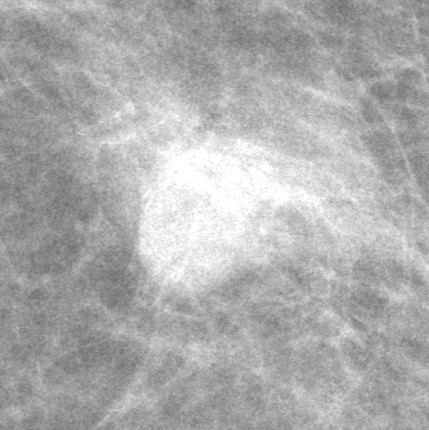
\includegraphics[width=\textwidth]{plots/breastMass.jpg}
			\end{subfigure}
			~
			\begin{subfigure}{0.35\textwidth}
				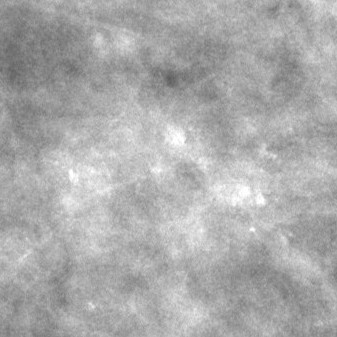
\includegraphics[width=\textwidth]{plots/breastMicrocalcification.jpg}
			\end{subfigure}
		\end{figure}

		Detection vs. diagnosis
	\end{frame}
		
	\begin{frame}
		\frametitle{Lesion segmentation}
		\begin{figure}[h]
			\centering
			\begin{subfigure}{0.35\textwidth}
				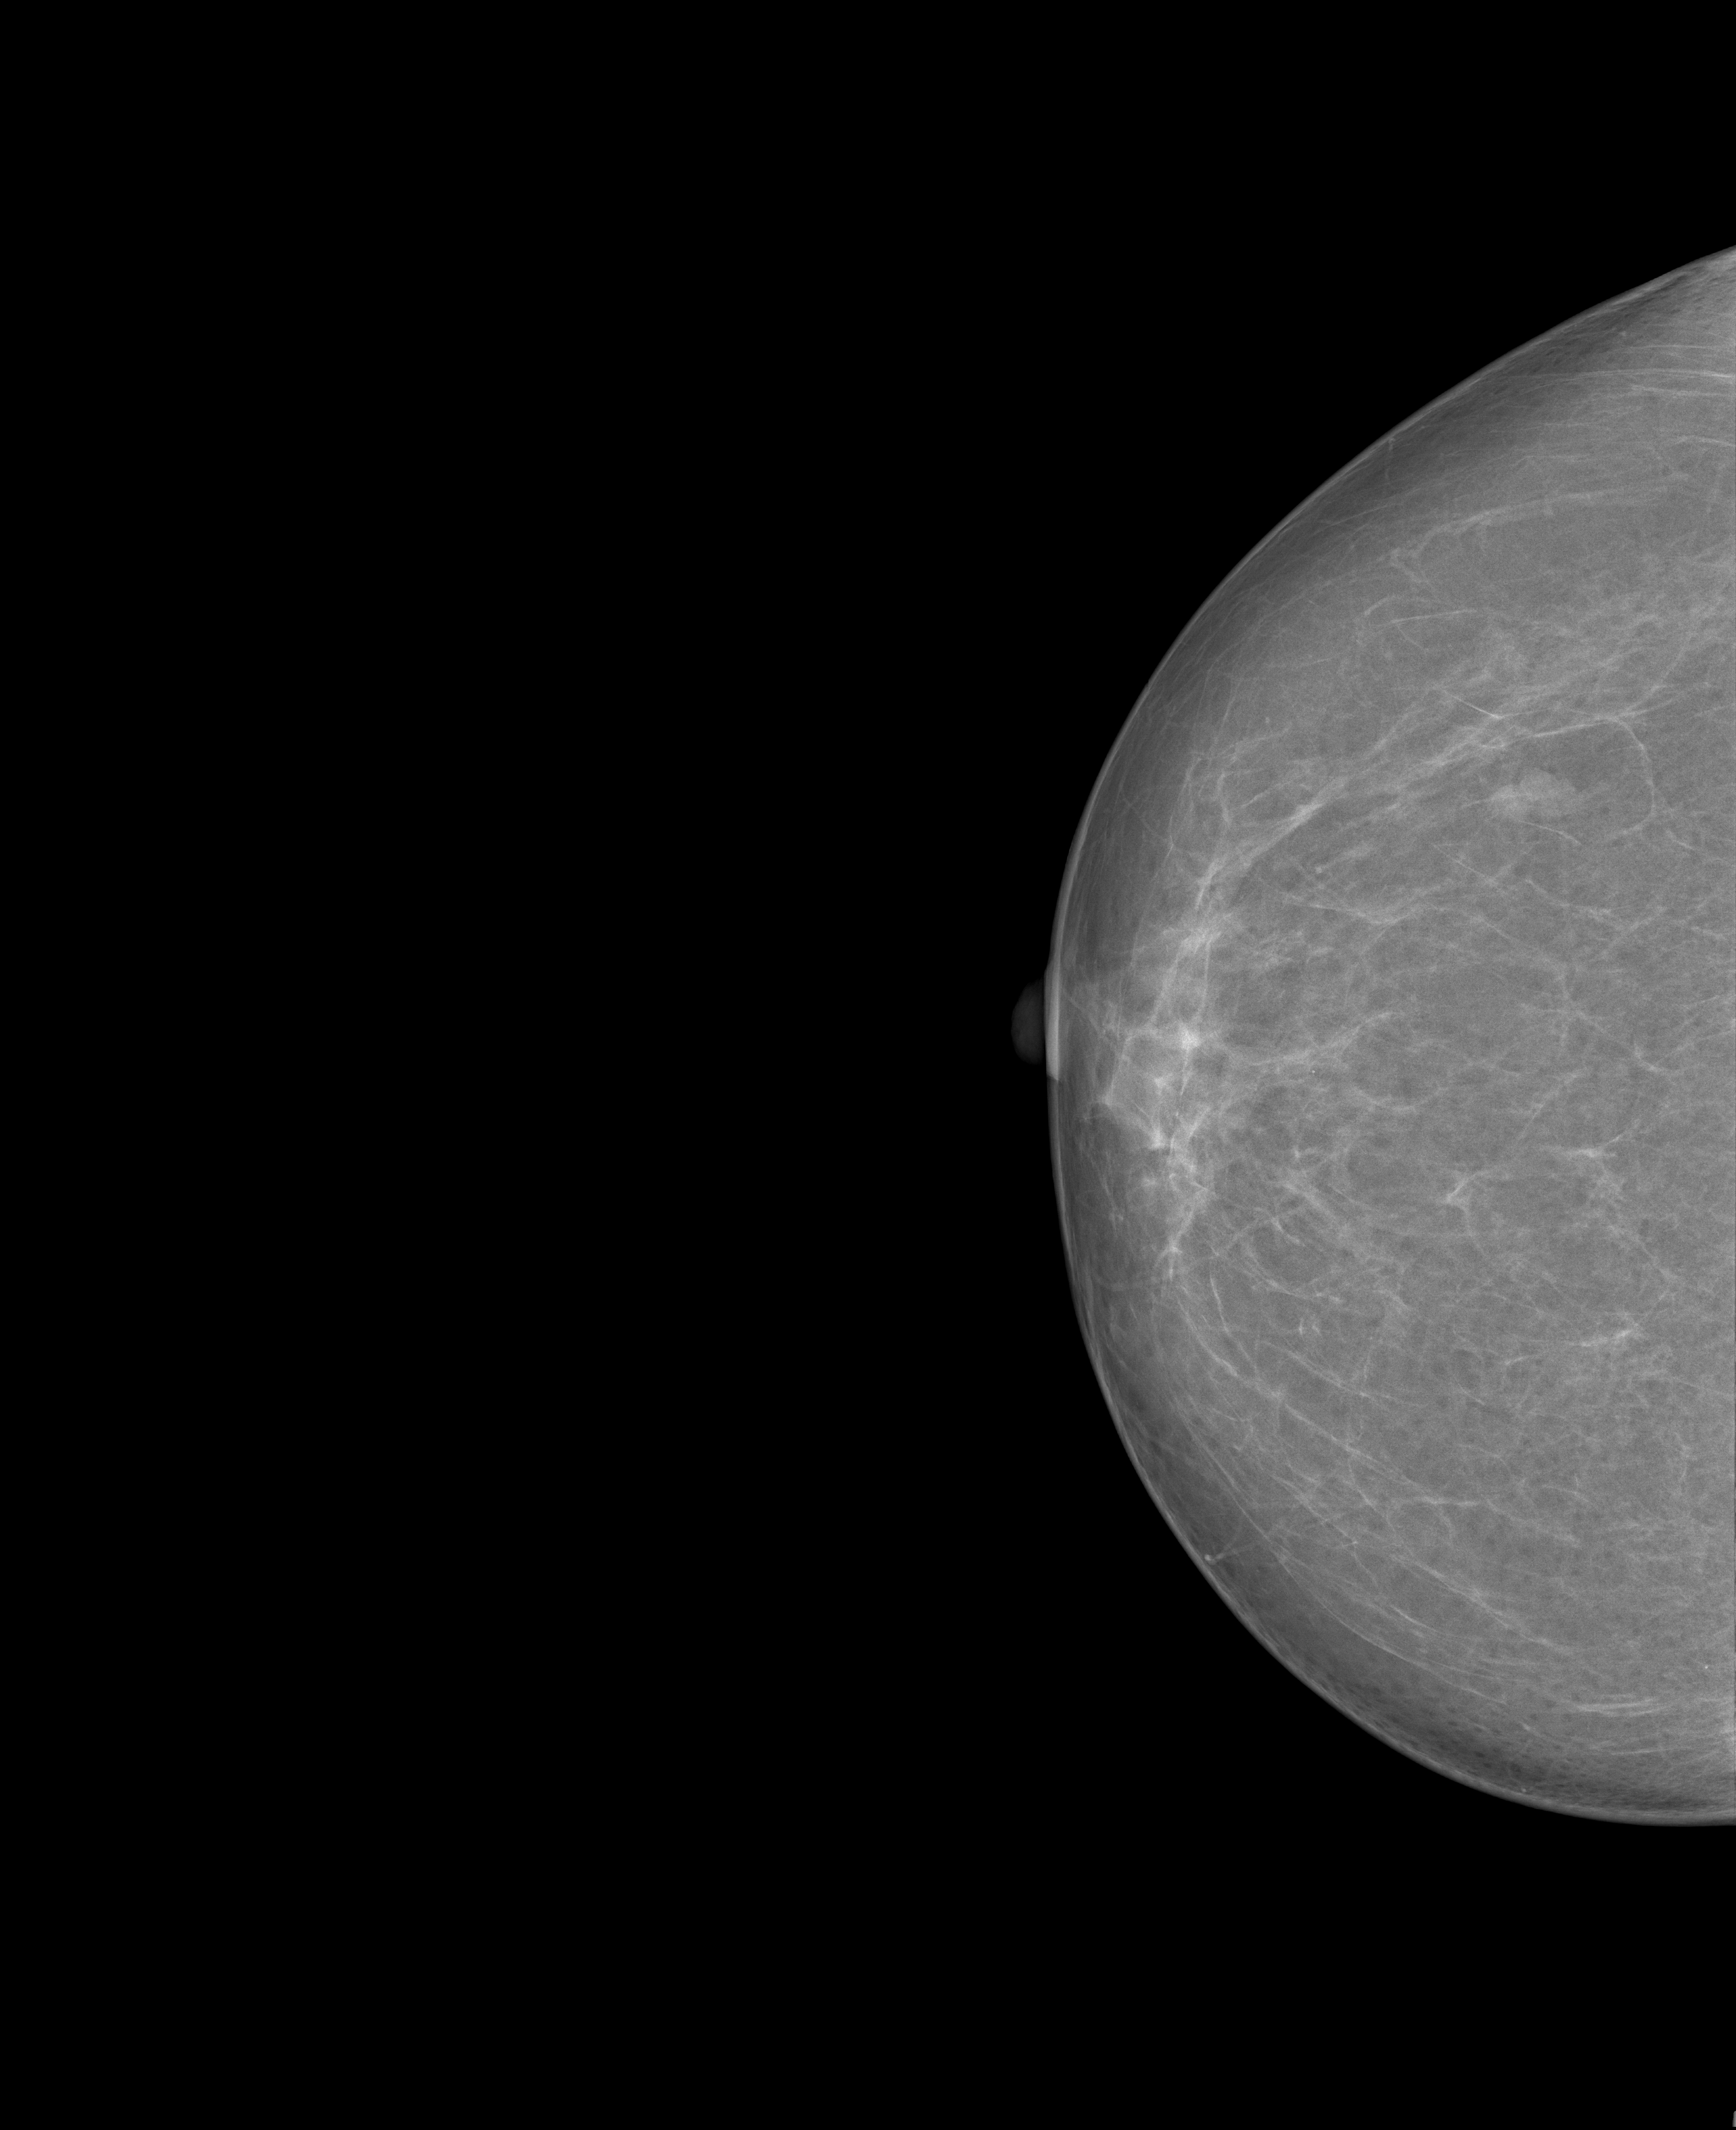
\includegraphics[width=\textwidth]{plots/mammogram.png}
				\caption{Mammogram}
			\end{subfigure}
			~
			\begin{subfigure}{0.35\textwidth}
				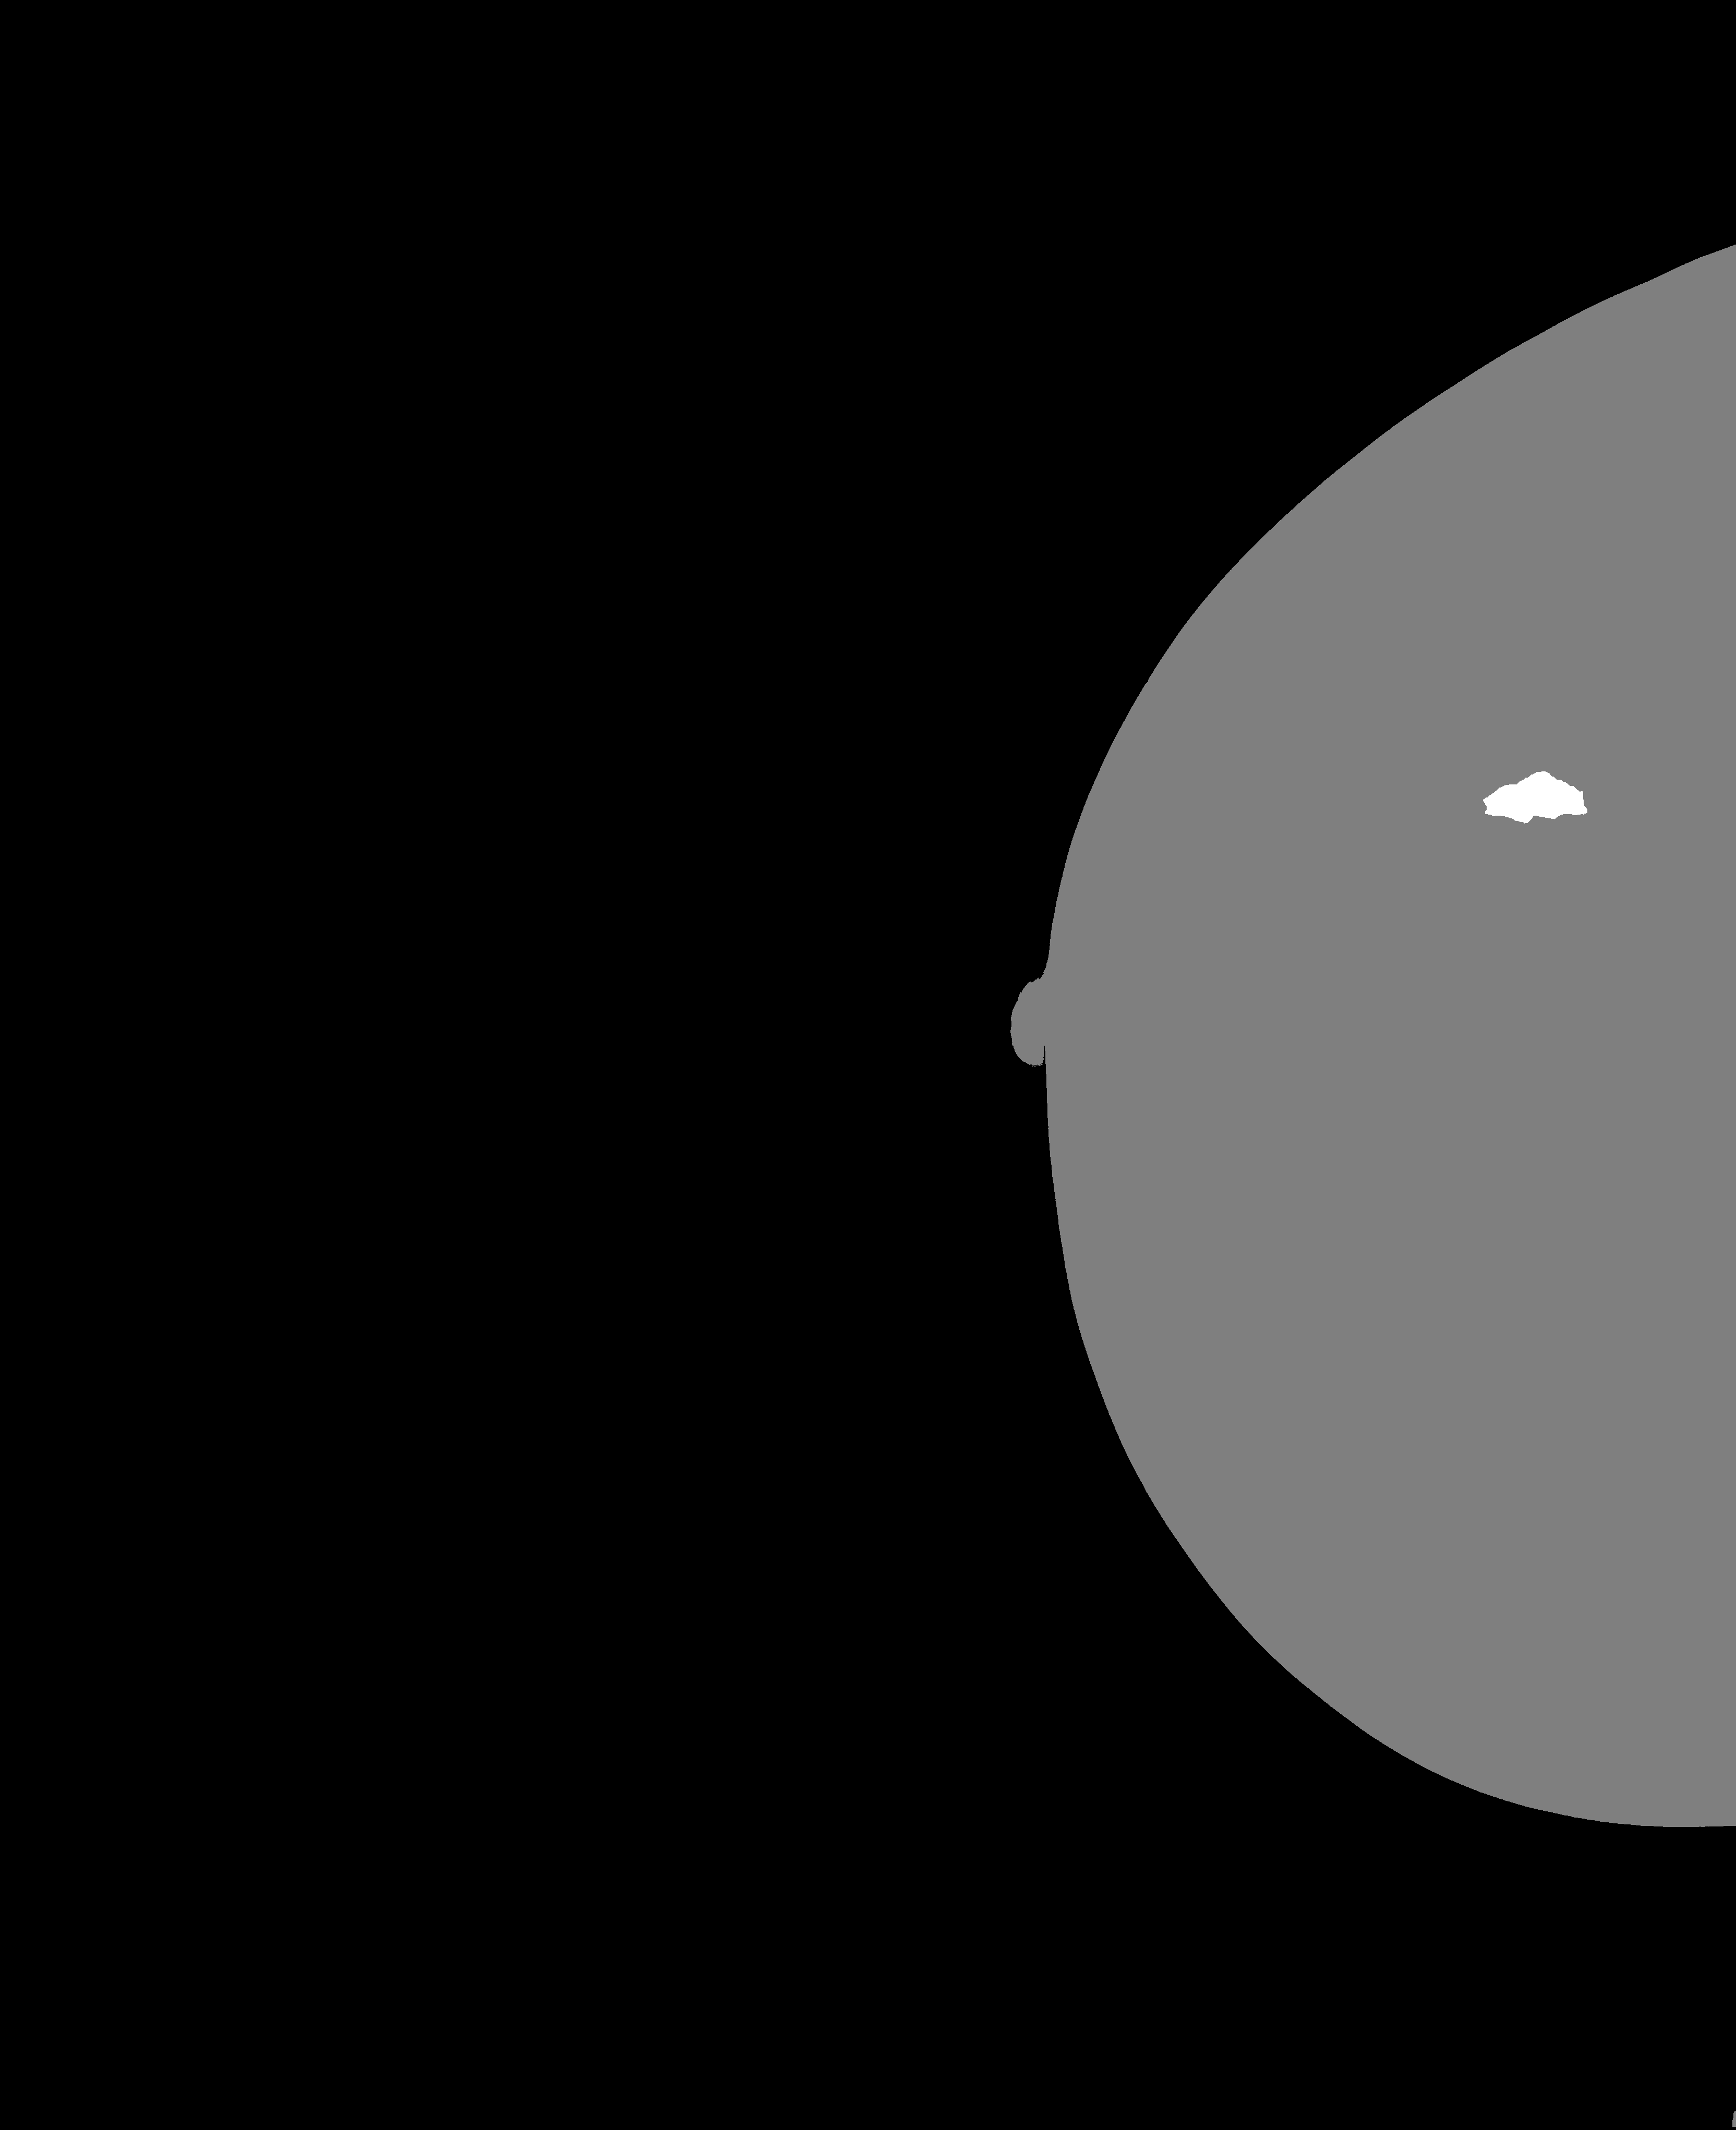
\includegraphics[width=\textwidth]{plots/label.png}
				\caption{Segmentation}
			\end{subfigure}
		% img_108_146_1_RCC.png
		\end{figure}
	\end{frame}
	
	
	\section[Convolutional networks]{Convolutional networks}
	\subsection[Classification]{Classification}
	\begin{frame}
		\vspace{30pt}
		\frametitle{Convolutional networks}
		\begin{figure}[h]
			\centering
			\begin{subfigure}{0.4\textwidth}
				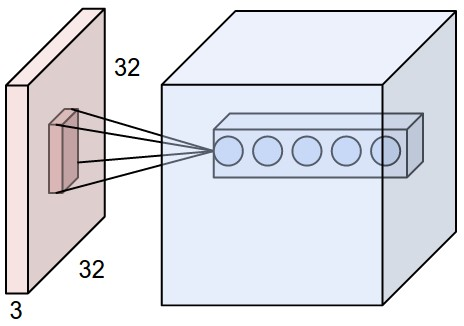
\includegraphics[width=\textwidth]{plots/convLayer.jpeg}
			\end{subfigure}
			~
			\begin{subfigure}{0.5\textwidth}
				\begin{subfigure}{\textwidth}
					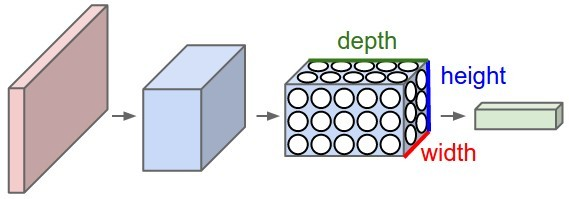
\includegraphics[width=\textwidth]{plots/convNetVolumes.jpeg}
				\end{subfigure}
				\par \smallskip
				\begin{subfigure}{\textwidth}
					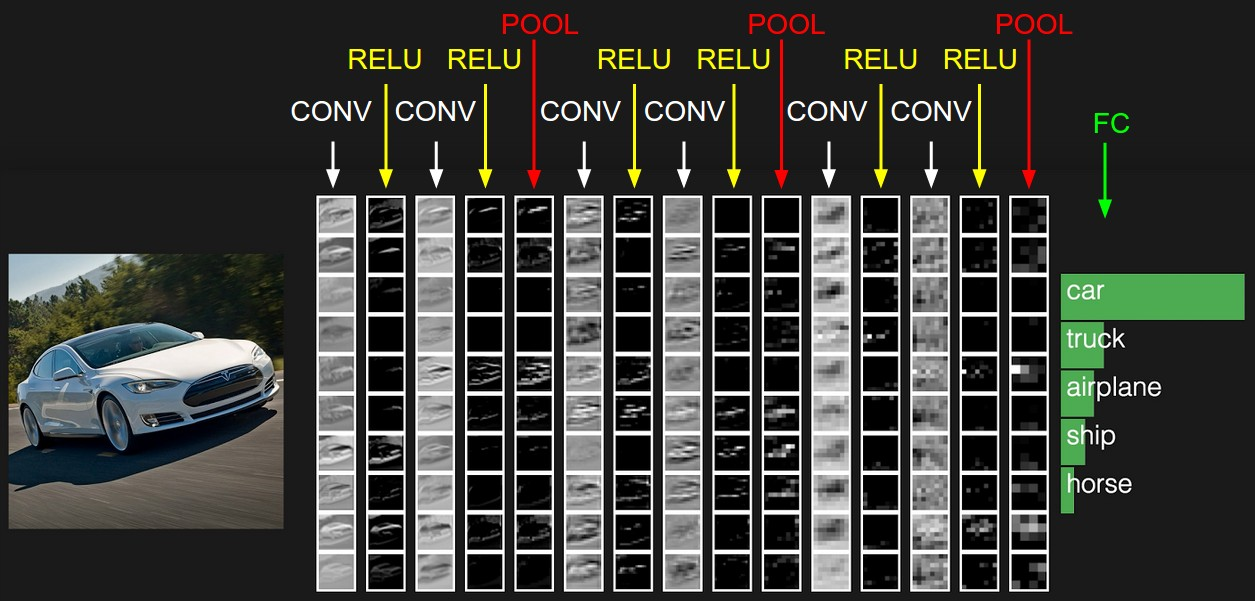
\includegraphics[width=\textwidth]{plots/convNetExample.jpeg}
				\end{subfigure}
			\end{subfigure}
		\end{figure}
		\source{[Karpathy et al., 2016]}
		% Explain kernels and hierarchichal features
	\end{frame}
		
	\begin{frame}
		\frametitle{What have they done}
		\vspace{30pt}
		\begin{figure}[h]
			\centering
			\begin{subfigure}{\textwidth}
				
\includegraphics[width=\textwidth]{plots/imageNetLogo.png}
			\end{subfigure}
			\par\smallskip
			\begin{subfigure}{0.35\textwidth}
				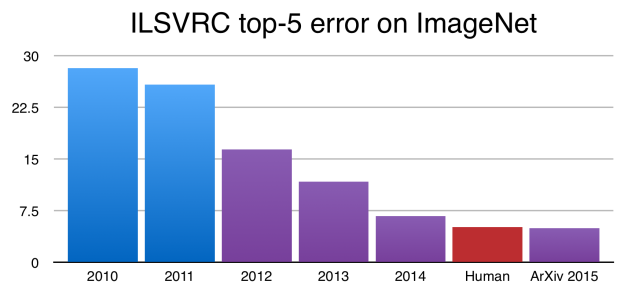
\includegraphics[width=\textwidth]{plots/imageNetAdvances.png}
			\end{subfigure}
			~
			\begin{subfigure}{0.6\textwidth}
				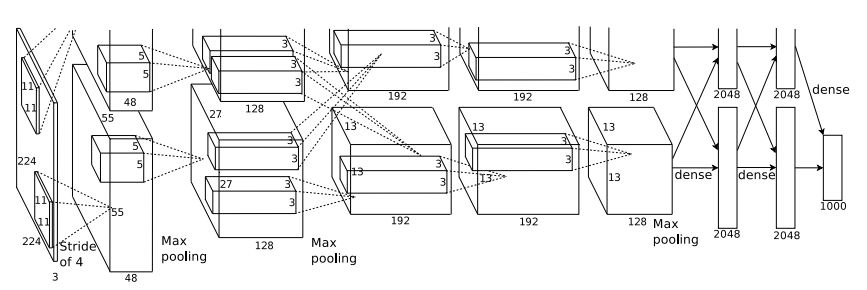
\includegraphics[width=\textwidth]{plots/alexnet.png}
			\end{subfigure}
		\end{figure}
		\source{[Nvidia Corp., 2015], [Krizhevsky et al., 2012]}
		% Explain ImageNet and talk about results
	\end{frame}
	
	\begin{frame}
		\frametitle{Architectures}
		\begin{figure}[h]
			\centering
			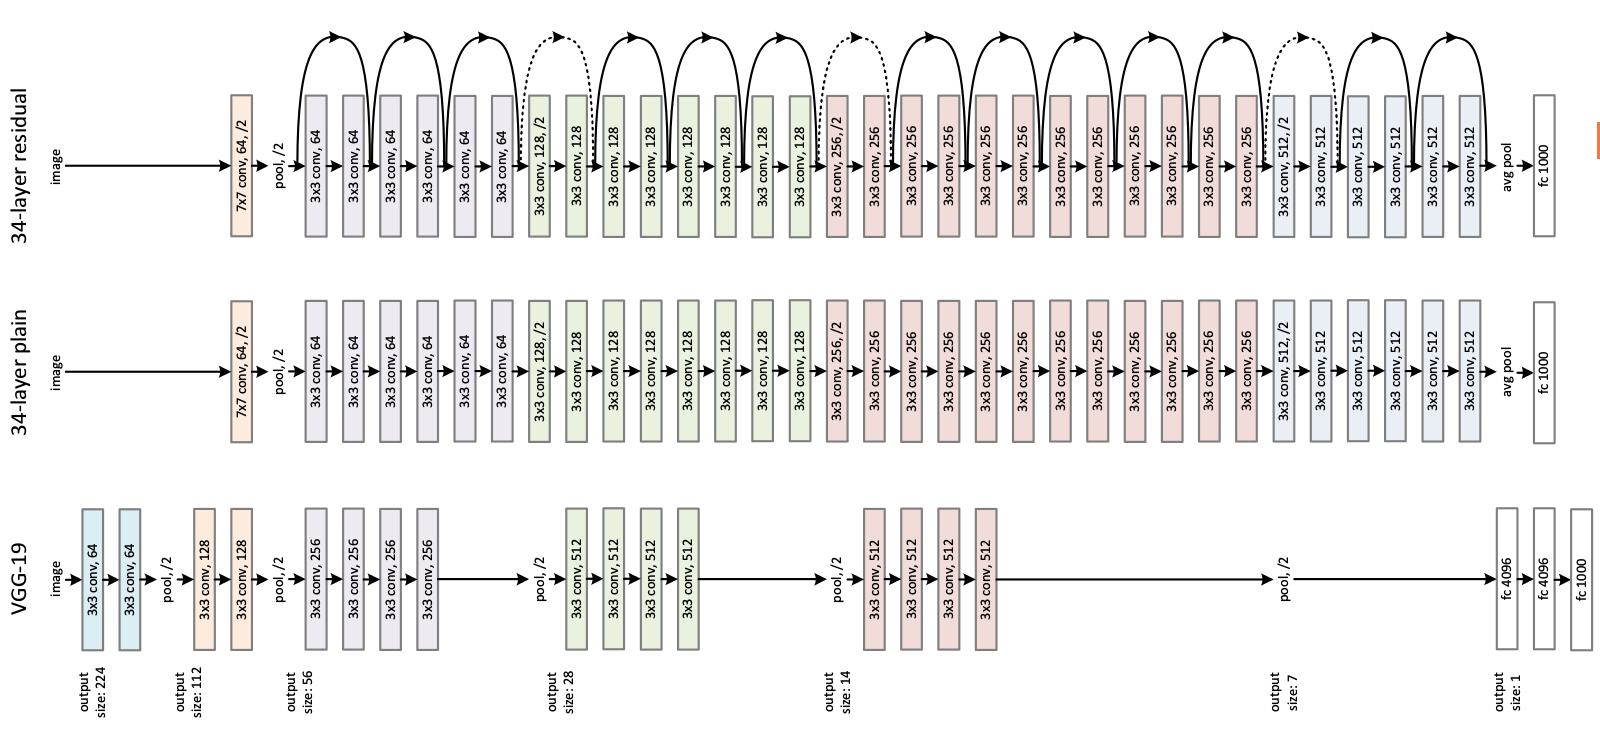
\includegraphics[width=\textwidth]{plots/resNet.png}
		\end{figure}
		
		Deeper, no pooling layers, no fully-connected layers, no dropout, all 3x3 kernels, batch normalization, residual connections,...
		\source{[He et al., 2015]}
		% VGG-net and ResNet-like/other things
		% Deeper, no pooling, no fc, no dropout, batchnorm, residual connections
		% all 3x3 convolutions
	\end{frame}
	

	\subsection[Segmentation]{Segmentation}
	\begin{frame}
		\frametitle{Segmentation}
		Solved by upsampling, deconvolution or dilated convolutions.
		\begin{figure}[h]
			\centering
			\begin{subfigure}{0.45\textwidth}
				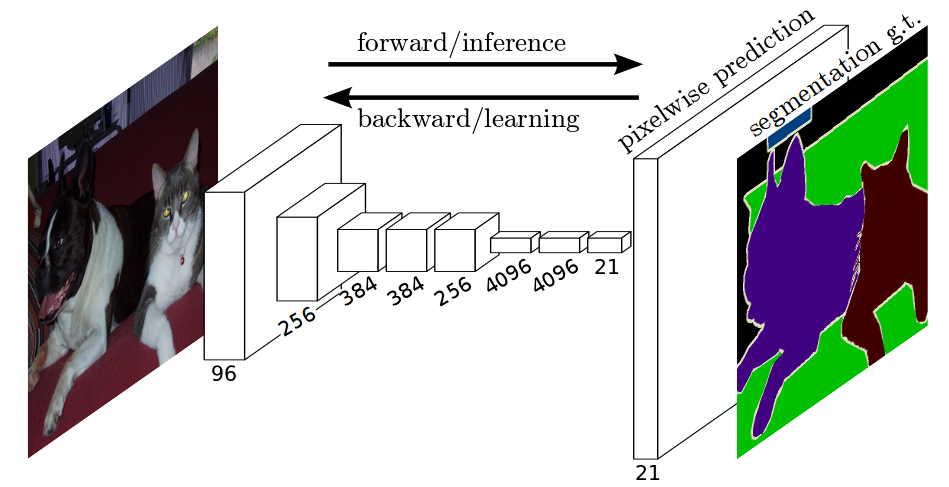
\includegraphics[width=\textwidth]{plots/fcn.png}
			\end{subfigure}
			~
			\begin{subfigure}{0.5\textwidth}
				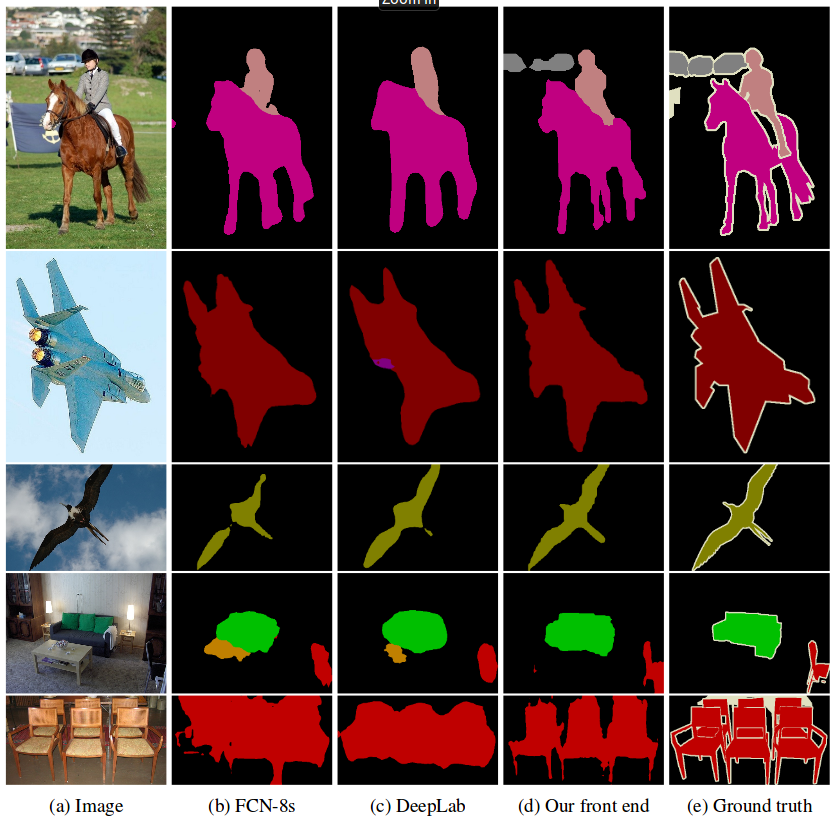
\includegraphics[width=\textwidth]{plots/segmentationComparison.png}
			\end{subfigure}
		\end{figure}
		\source{[Longet al., 2015], [Yu and Koltun, 2016]}
		% Explain how kernels are moved along ot produce a full result
	\end{frame}


	\section[Work done]{Work done}
	\begin{frame}
		\frametitle{Literature review}
		\vspace{15pt}
		\begin{figure}[h]
			\centering
			\begin{subfigure}{0.48\textwidth}
				\begin{subfigure}{\textwidth}
					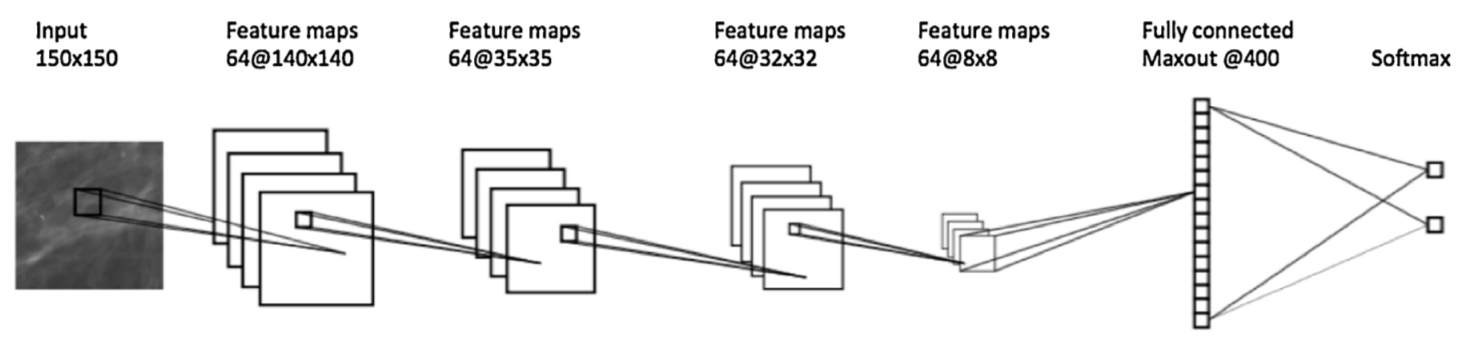
\includegraphics[width=\textwidth]{plots/arevalo.png}
				\end{subfigure}
				~
				\begin{subfigure}{\textwidth}
					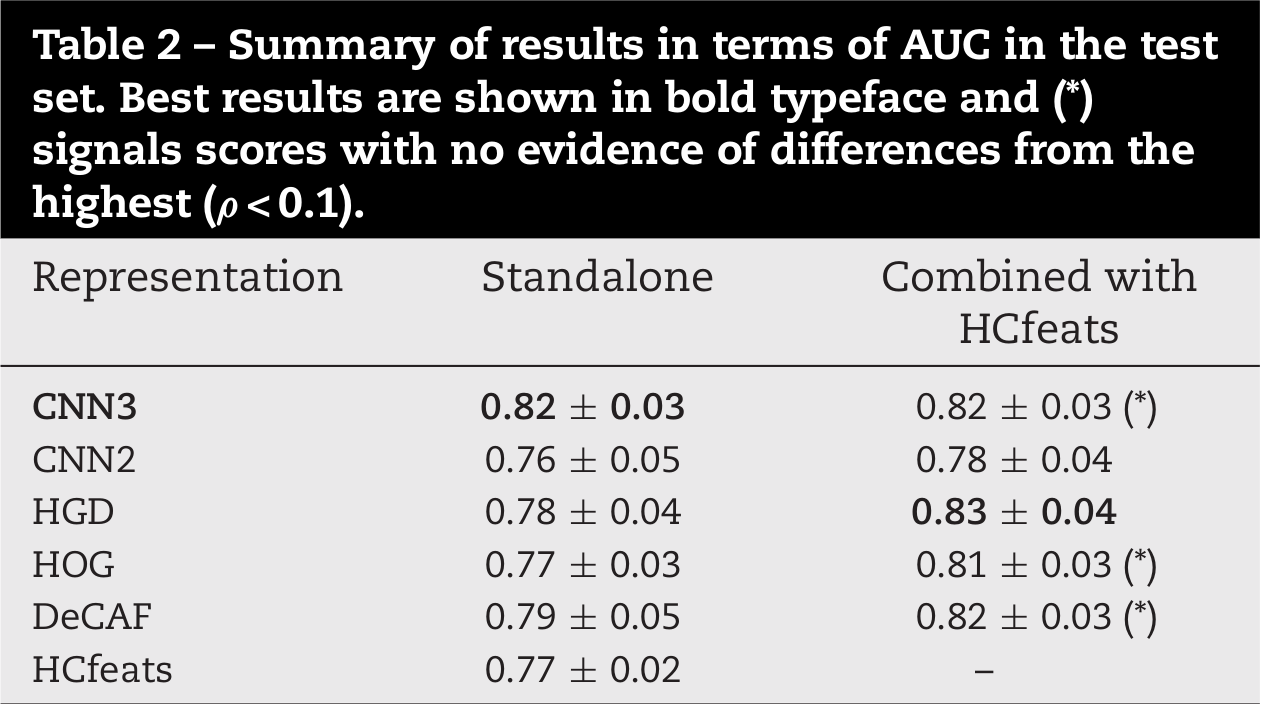
\includegraphics[width=\textwidth]{plots/arevaloResults.png}
				\end{subfigure}
				\caption{Mass diagnosis (4 layers, 3.4M params)}
			\end{subfigure}
			~
			\begin{subfigure}{0.48\textwidth}
				\begin{subfigure}{\textwidth}
					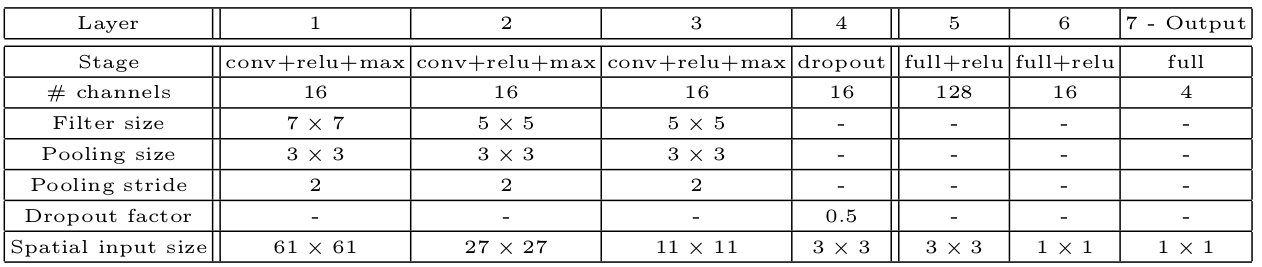
\includegraphics[width=\textwidth]{plots/dubrovina1.png}
				\end{subfigure}
				~
				\begin{subfigure}{\textwidth}
					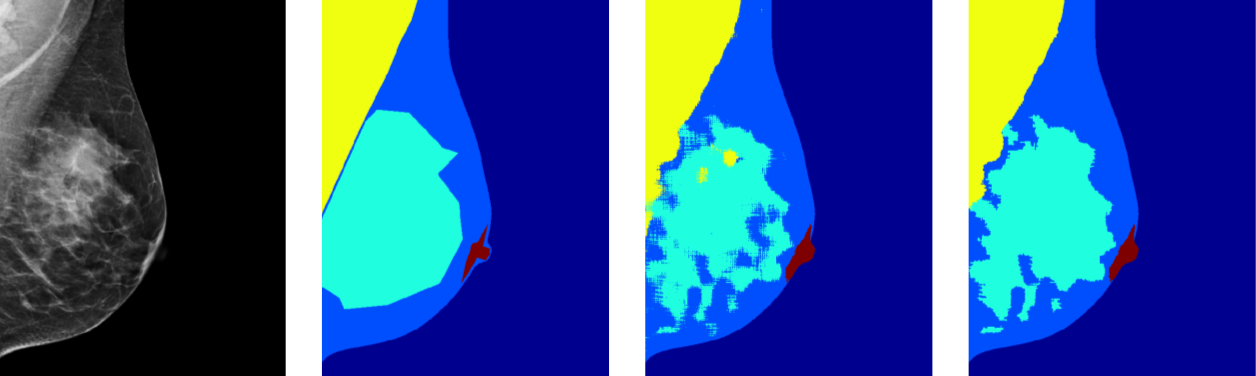
\includegraphics[width=\textwidth]{plots/dubrovina2.png}
				\end{subfigure}
				~
				\begin{subfigure}{\textwidth}
					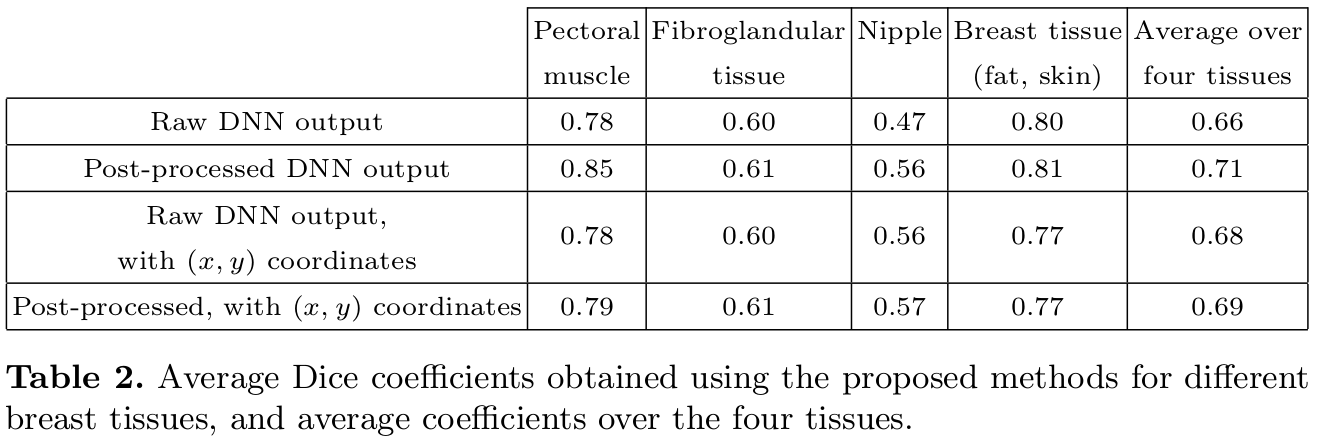
\includegraphics[width=\textwidth]{plots/dubrovinaResults.png}
				\end{subfigure}
				\caption{Tissue segmentation (6 layers, 34K params)}
			\end{subfigure}
		\end{figure}
		\source{[Arevalo et al., 2016], [Dubrovina et al.,2015]}
		% What has been done in breast cancer, Wrote background, examples and accuracies
	\end{frame}
	
	\begin{frame}
		\frametitle{Database preprocessing}
		\begin{figure}[h]
		\centering
			\begin{subfigure}{0.24\textwidth}
				\centering
					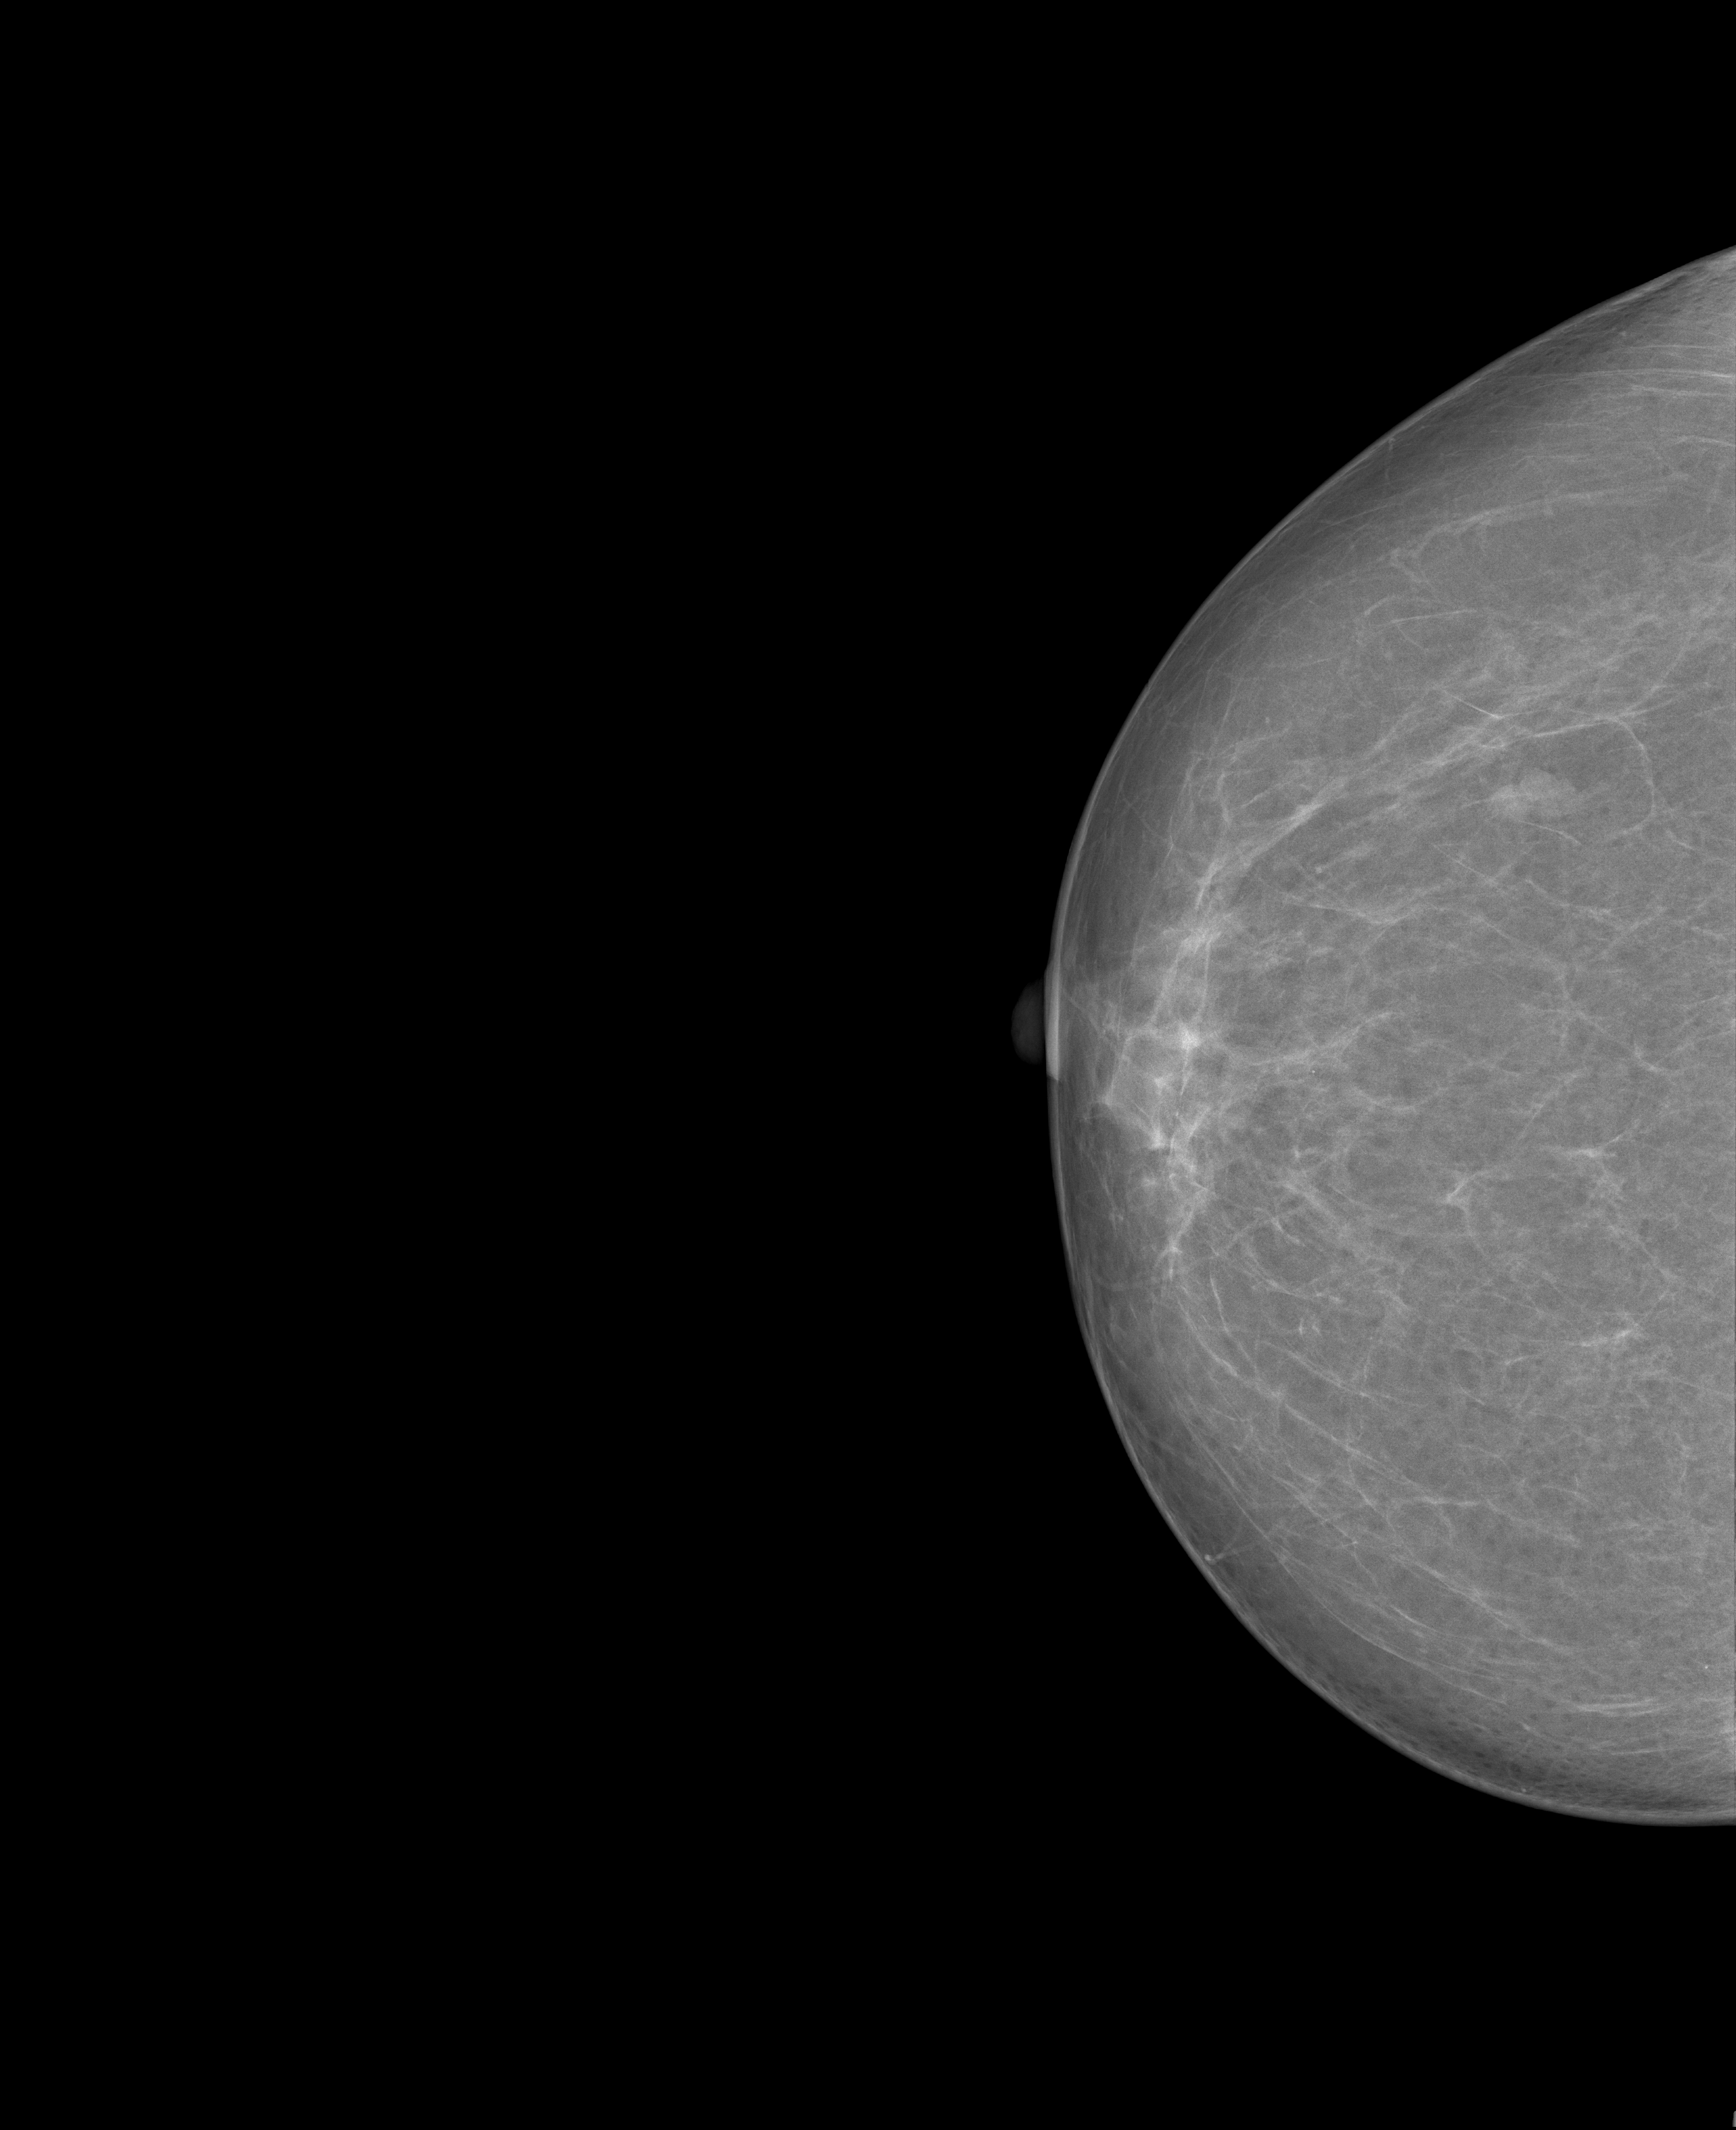
\includegraphics[height=3.5cm]{plots/mammogram.png}
			\end{subfigure}
			\begin{subfigure}{0.24\textwidth}
				\centering
					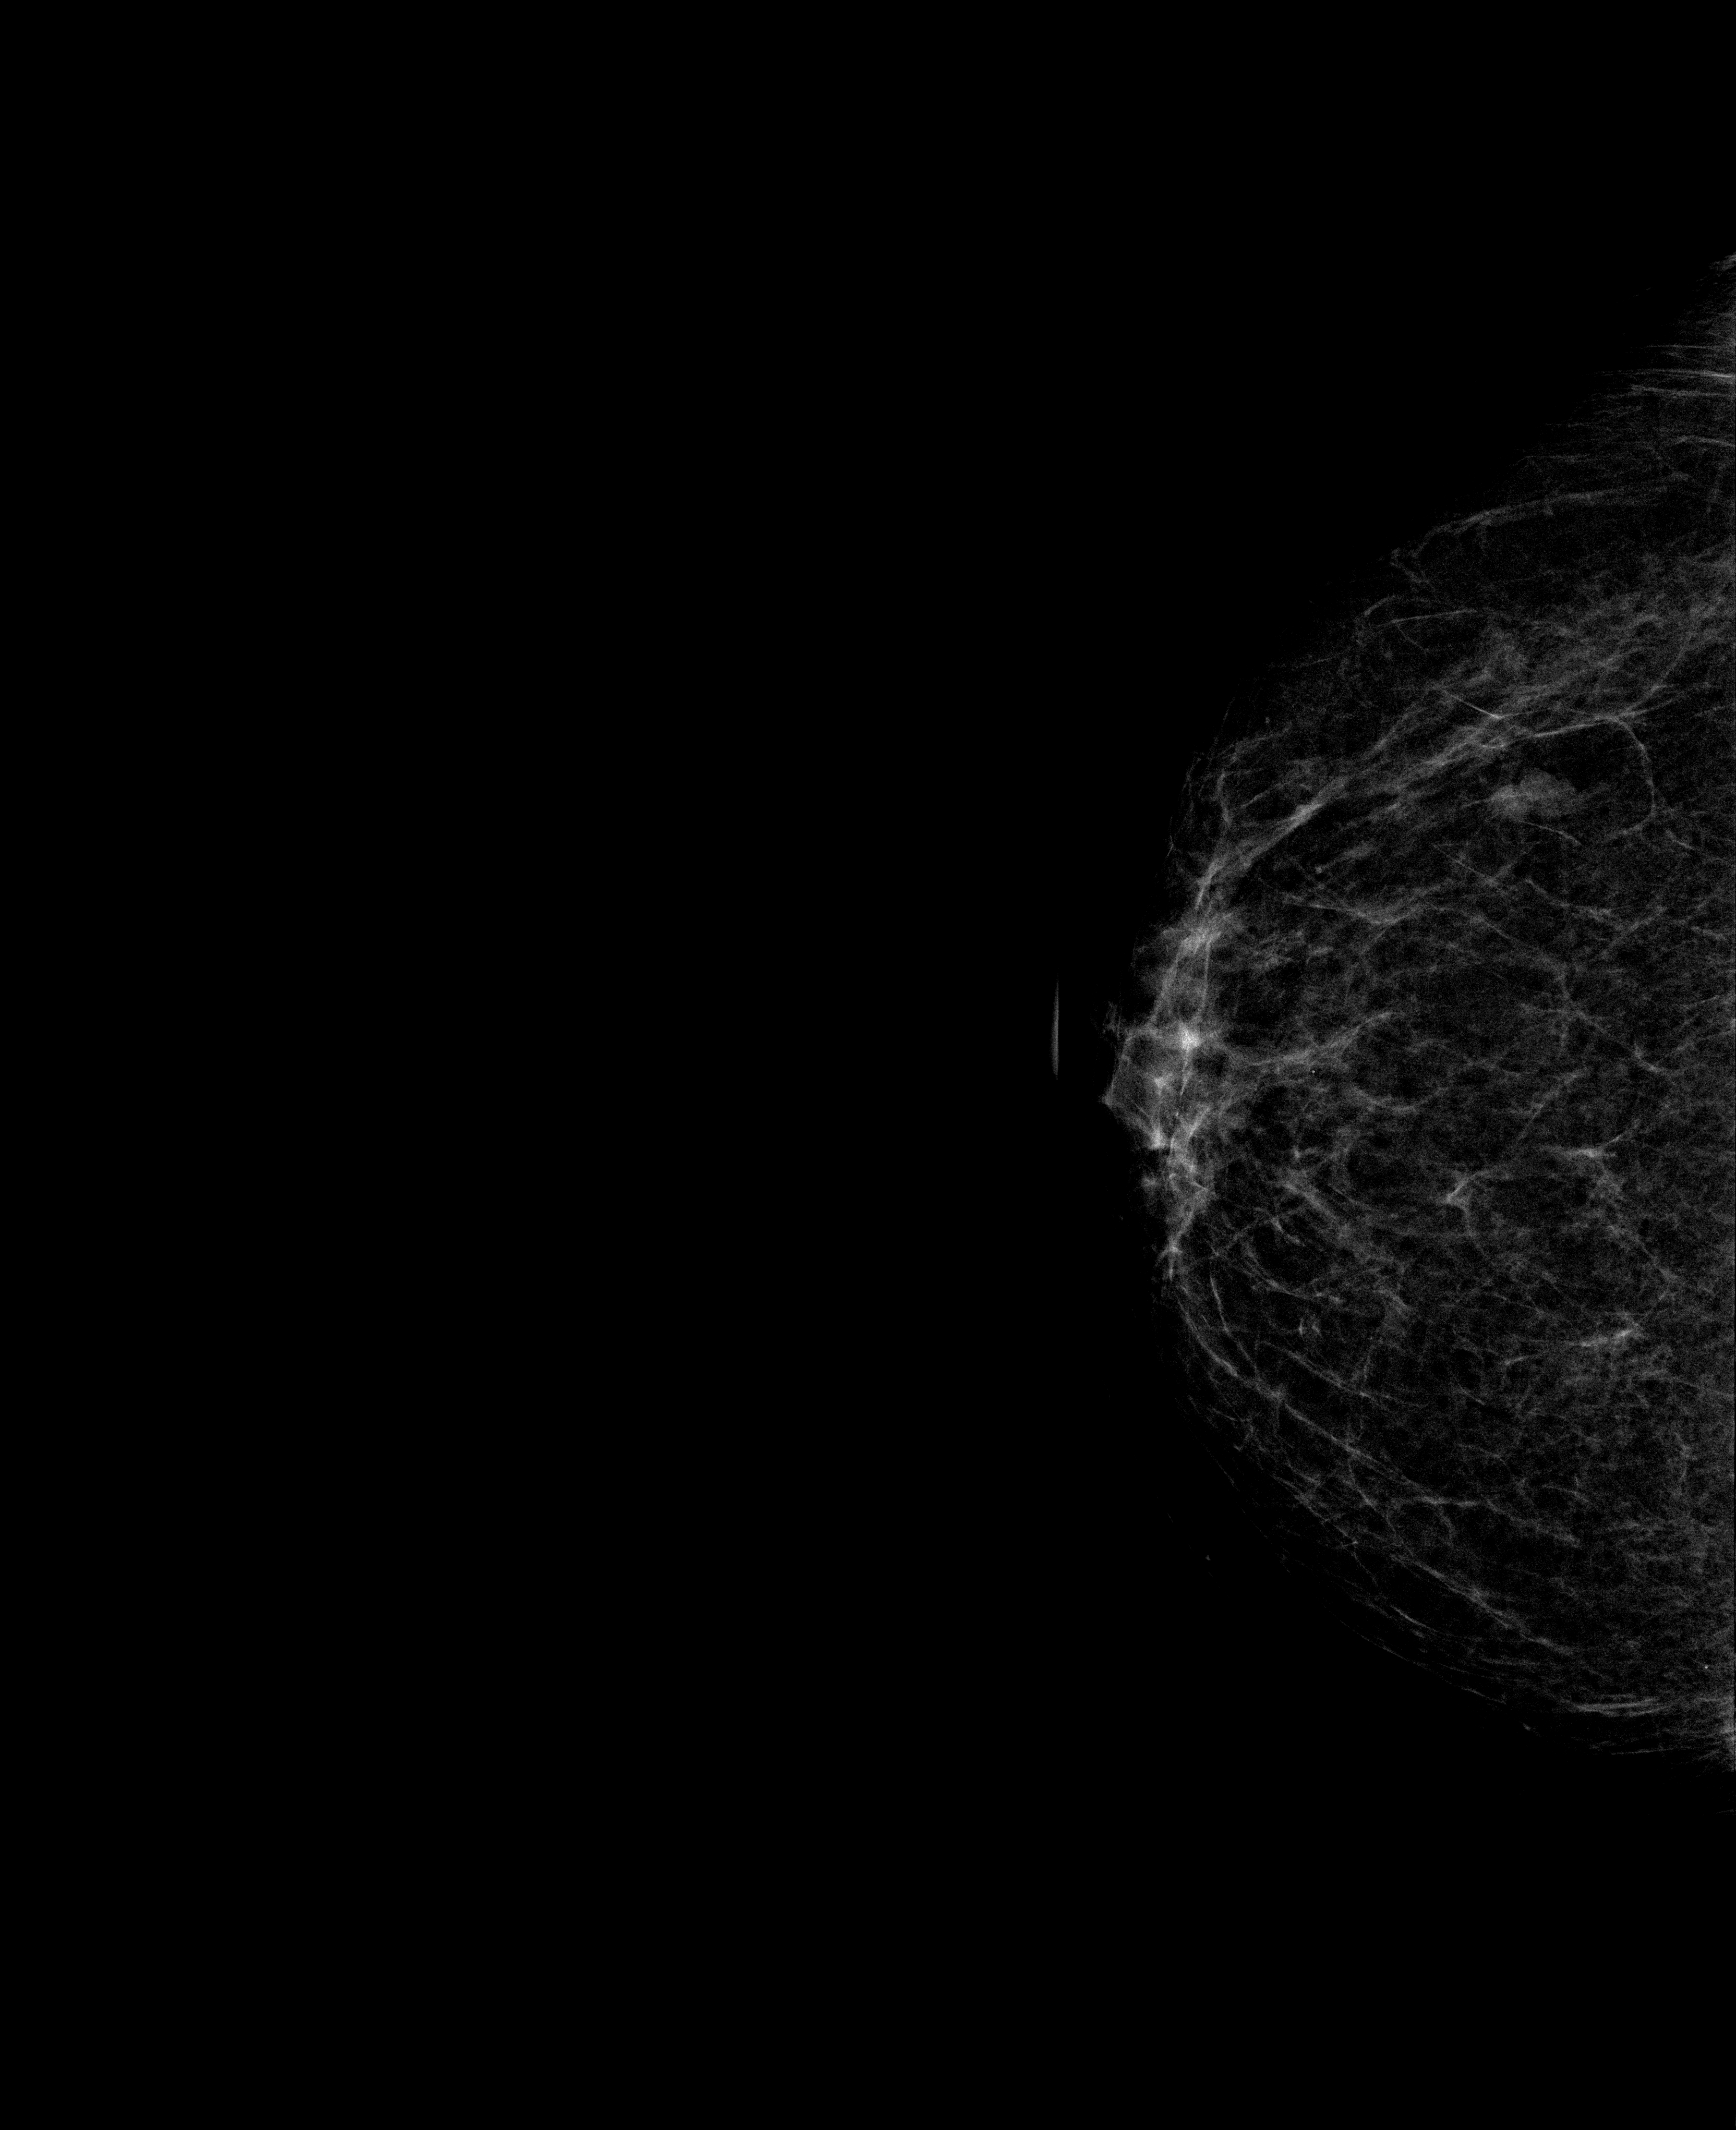
\includegraphics[height=3.5cm]{plots/mammogram_enhanced.png}
			\end{subfigure}
			\begin{subfigure}{0.24\textwidth}
				\centering
					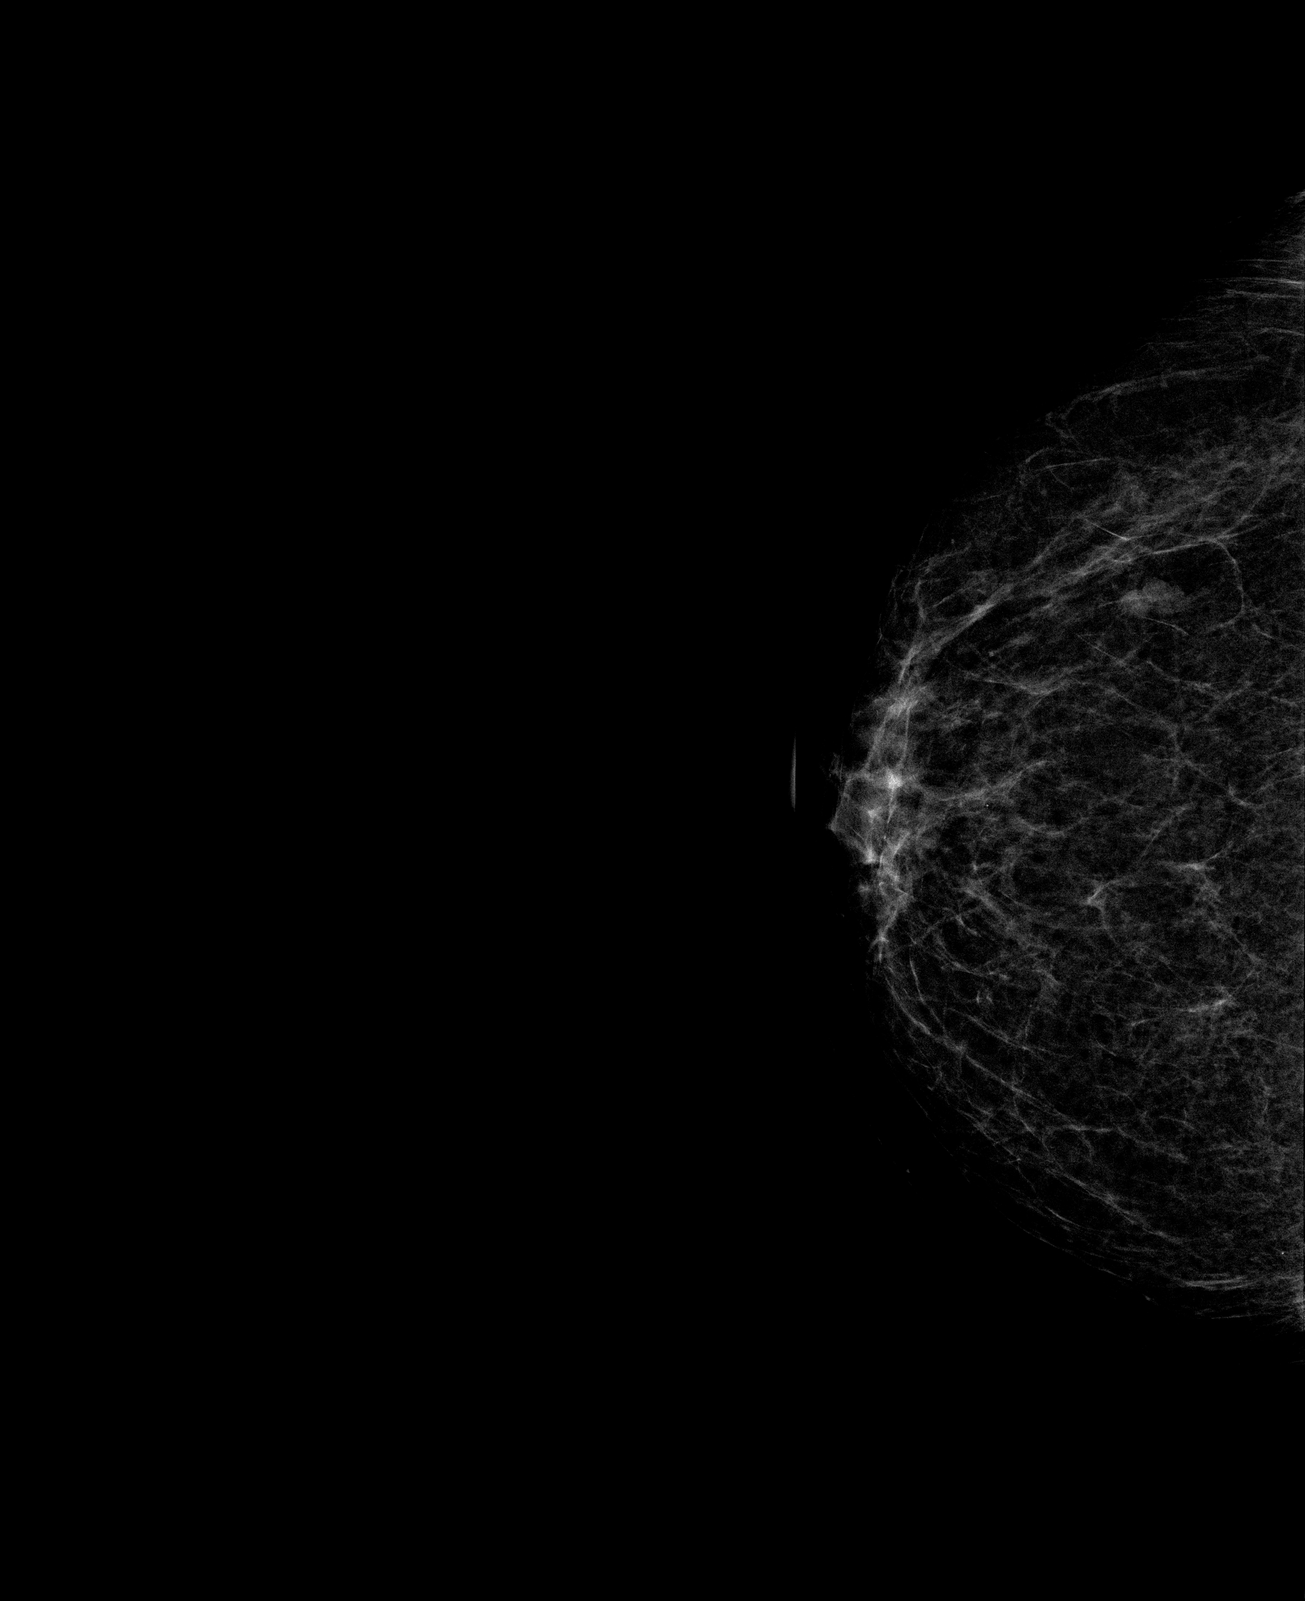
\includegraphics[height=3.5cm]{plots/mammogram_resized.png}
			\end{subfigure}
			\begin{subfigure}{0.11\textwidth}
				\centering
					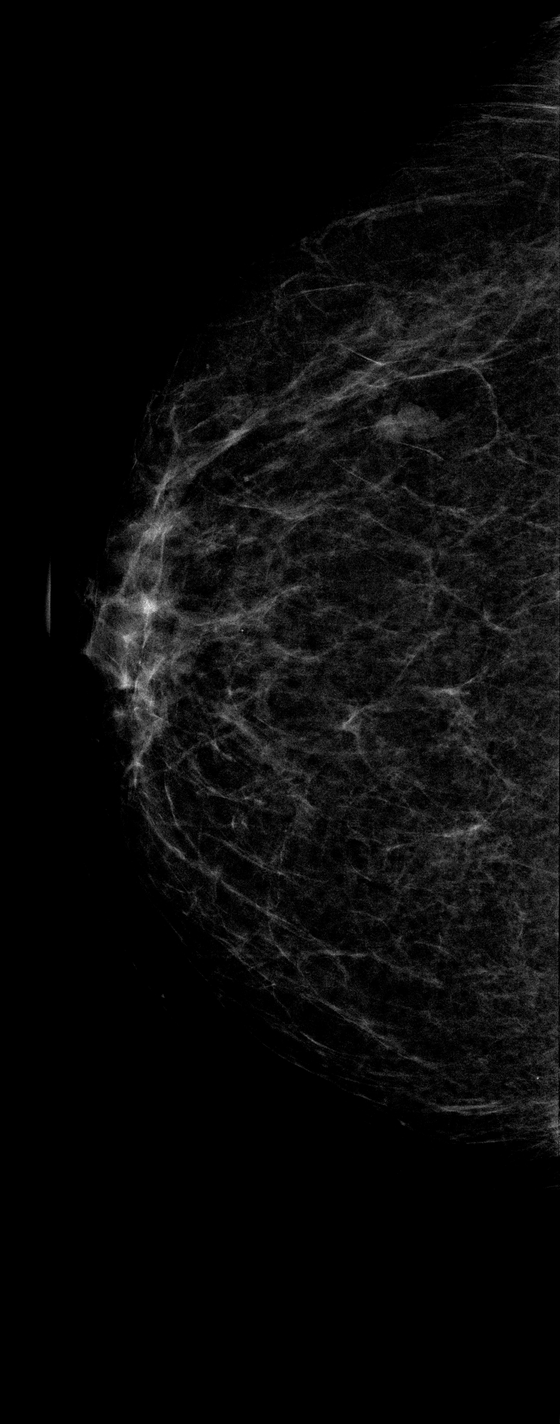
\includegraphics[height=3.5cm]{plots/mammogram_v1.png}
			\end{subfigure}
			~
			\begin{subfigure}{0.24\textwidth}
				\centering
					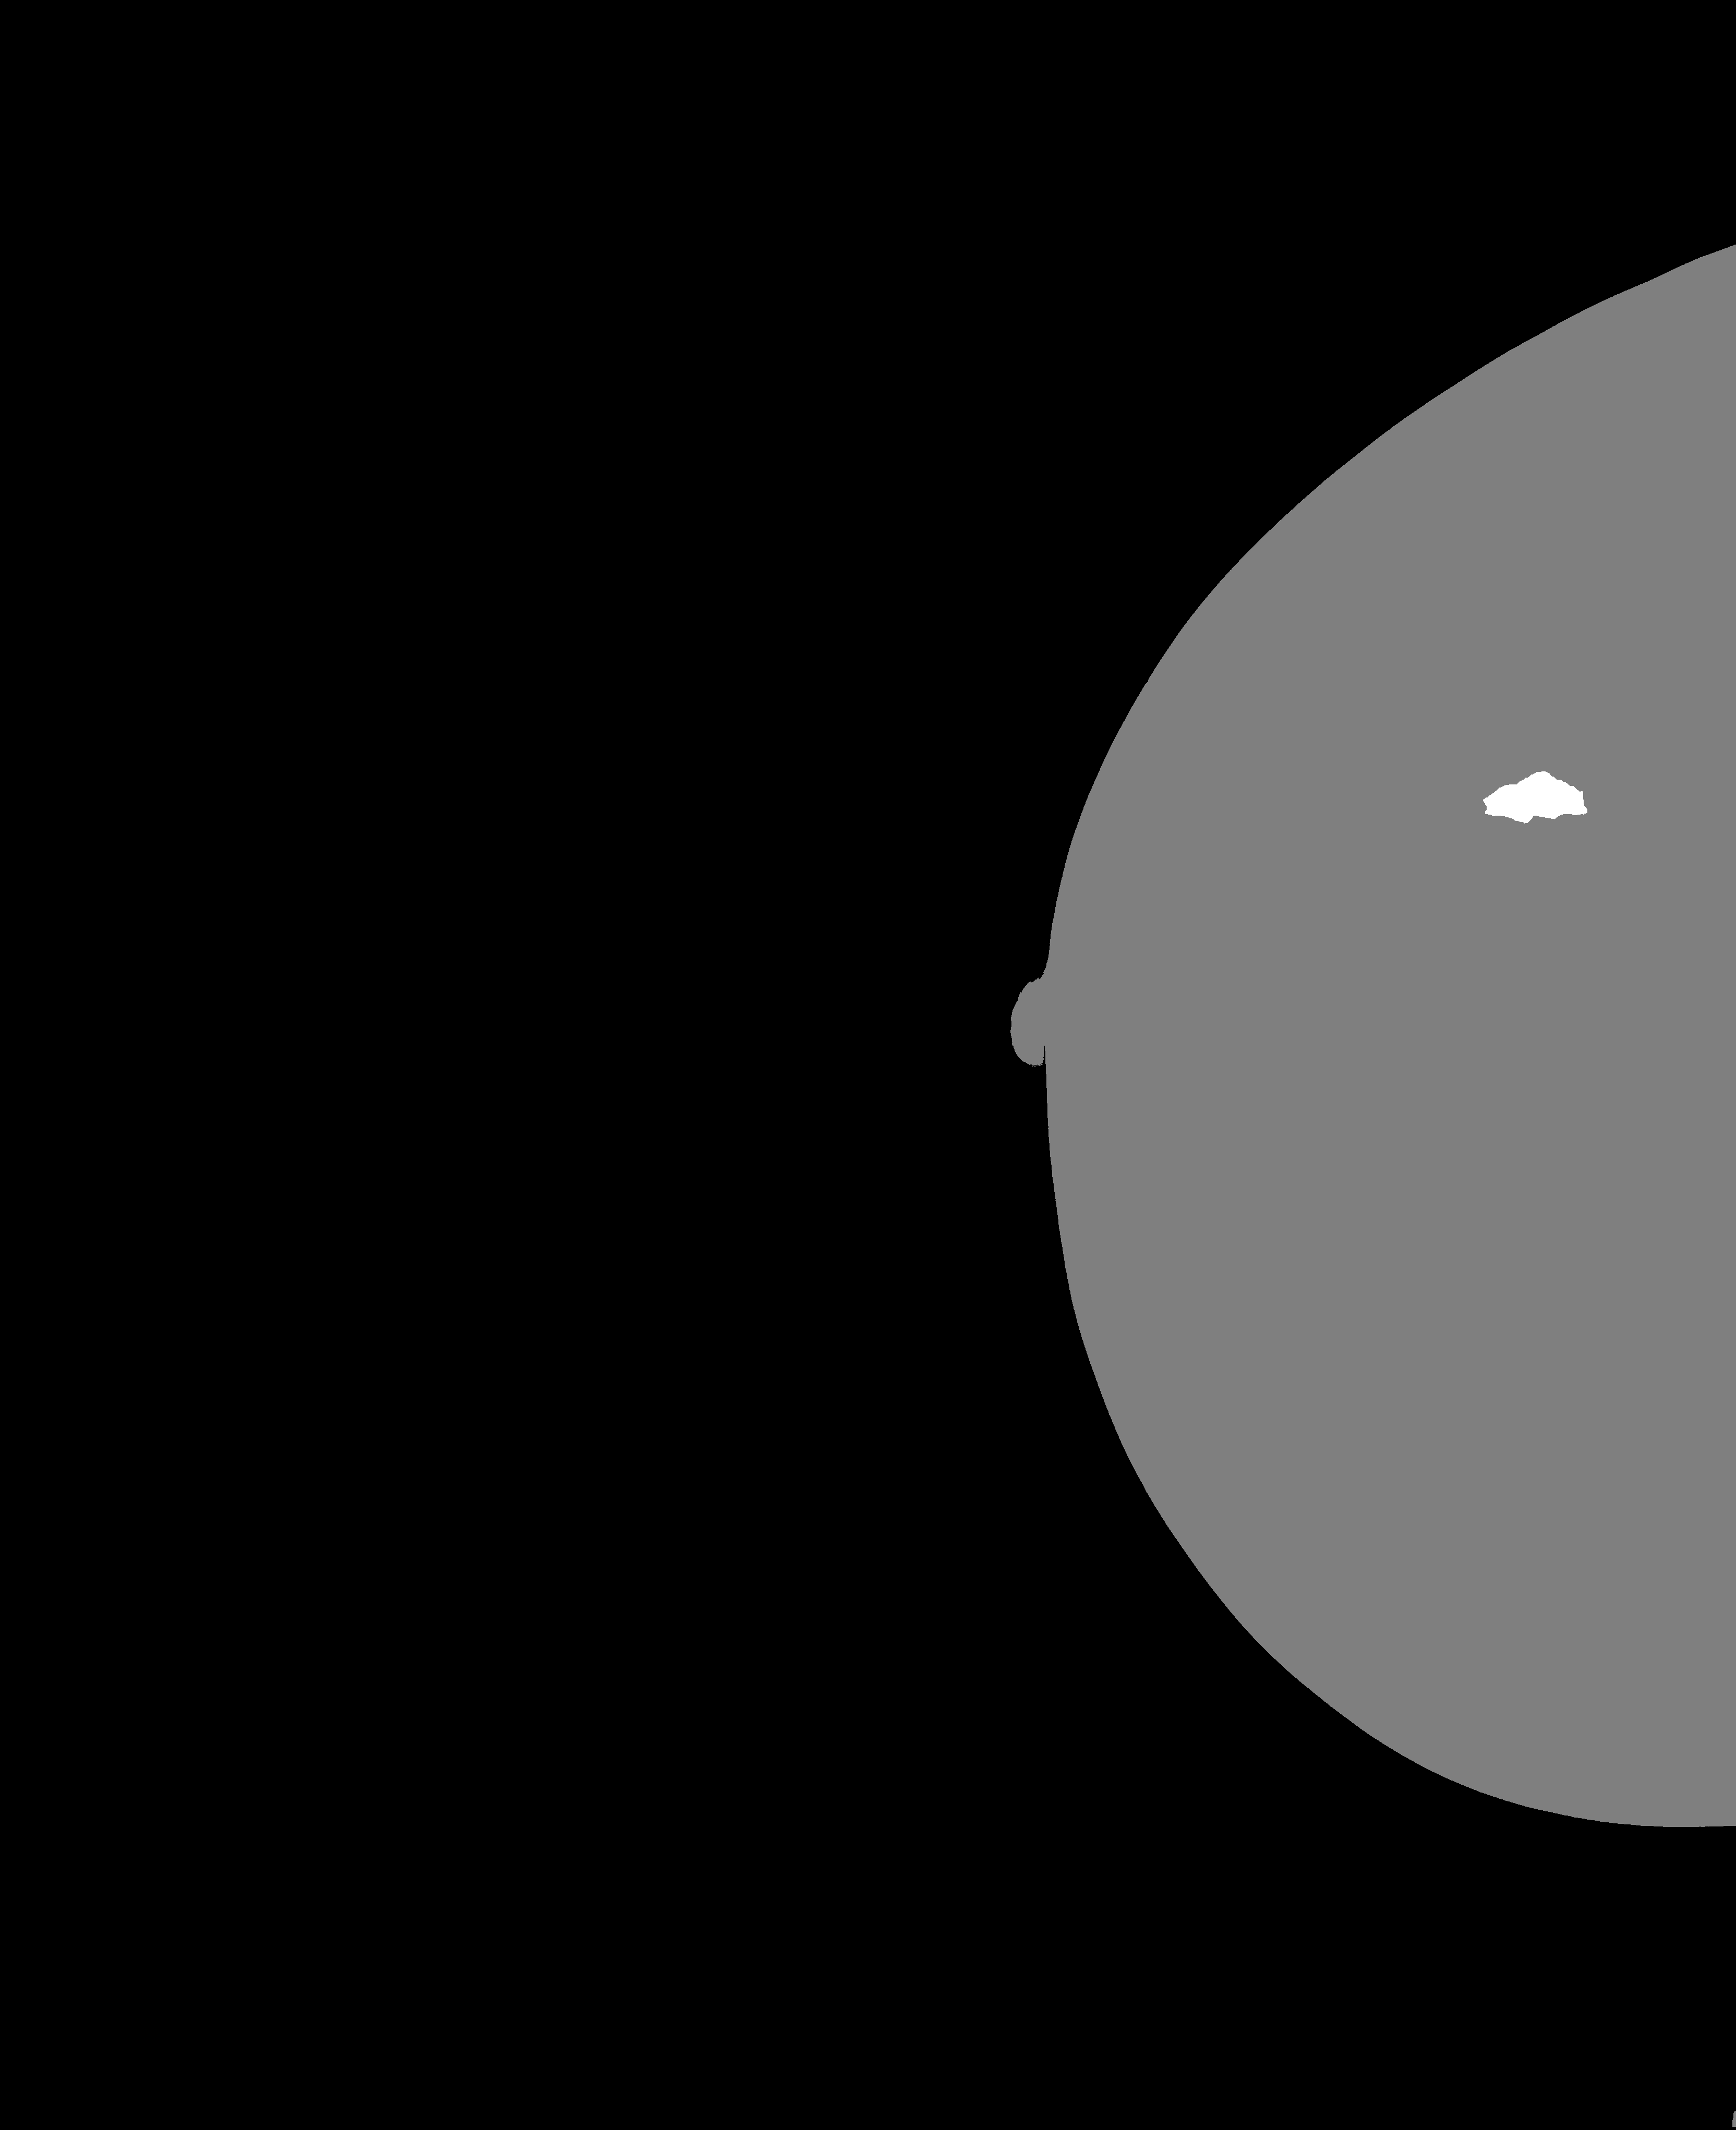
\includegraphics[height = 3.5cm]{plots/label.png}
				\caption{Original image}
				\label{subfig:Preprocessinga}
			\end{subfigure}
			\begin{subfigure}{0.24\textwidth}
				\centering
					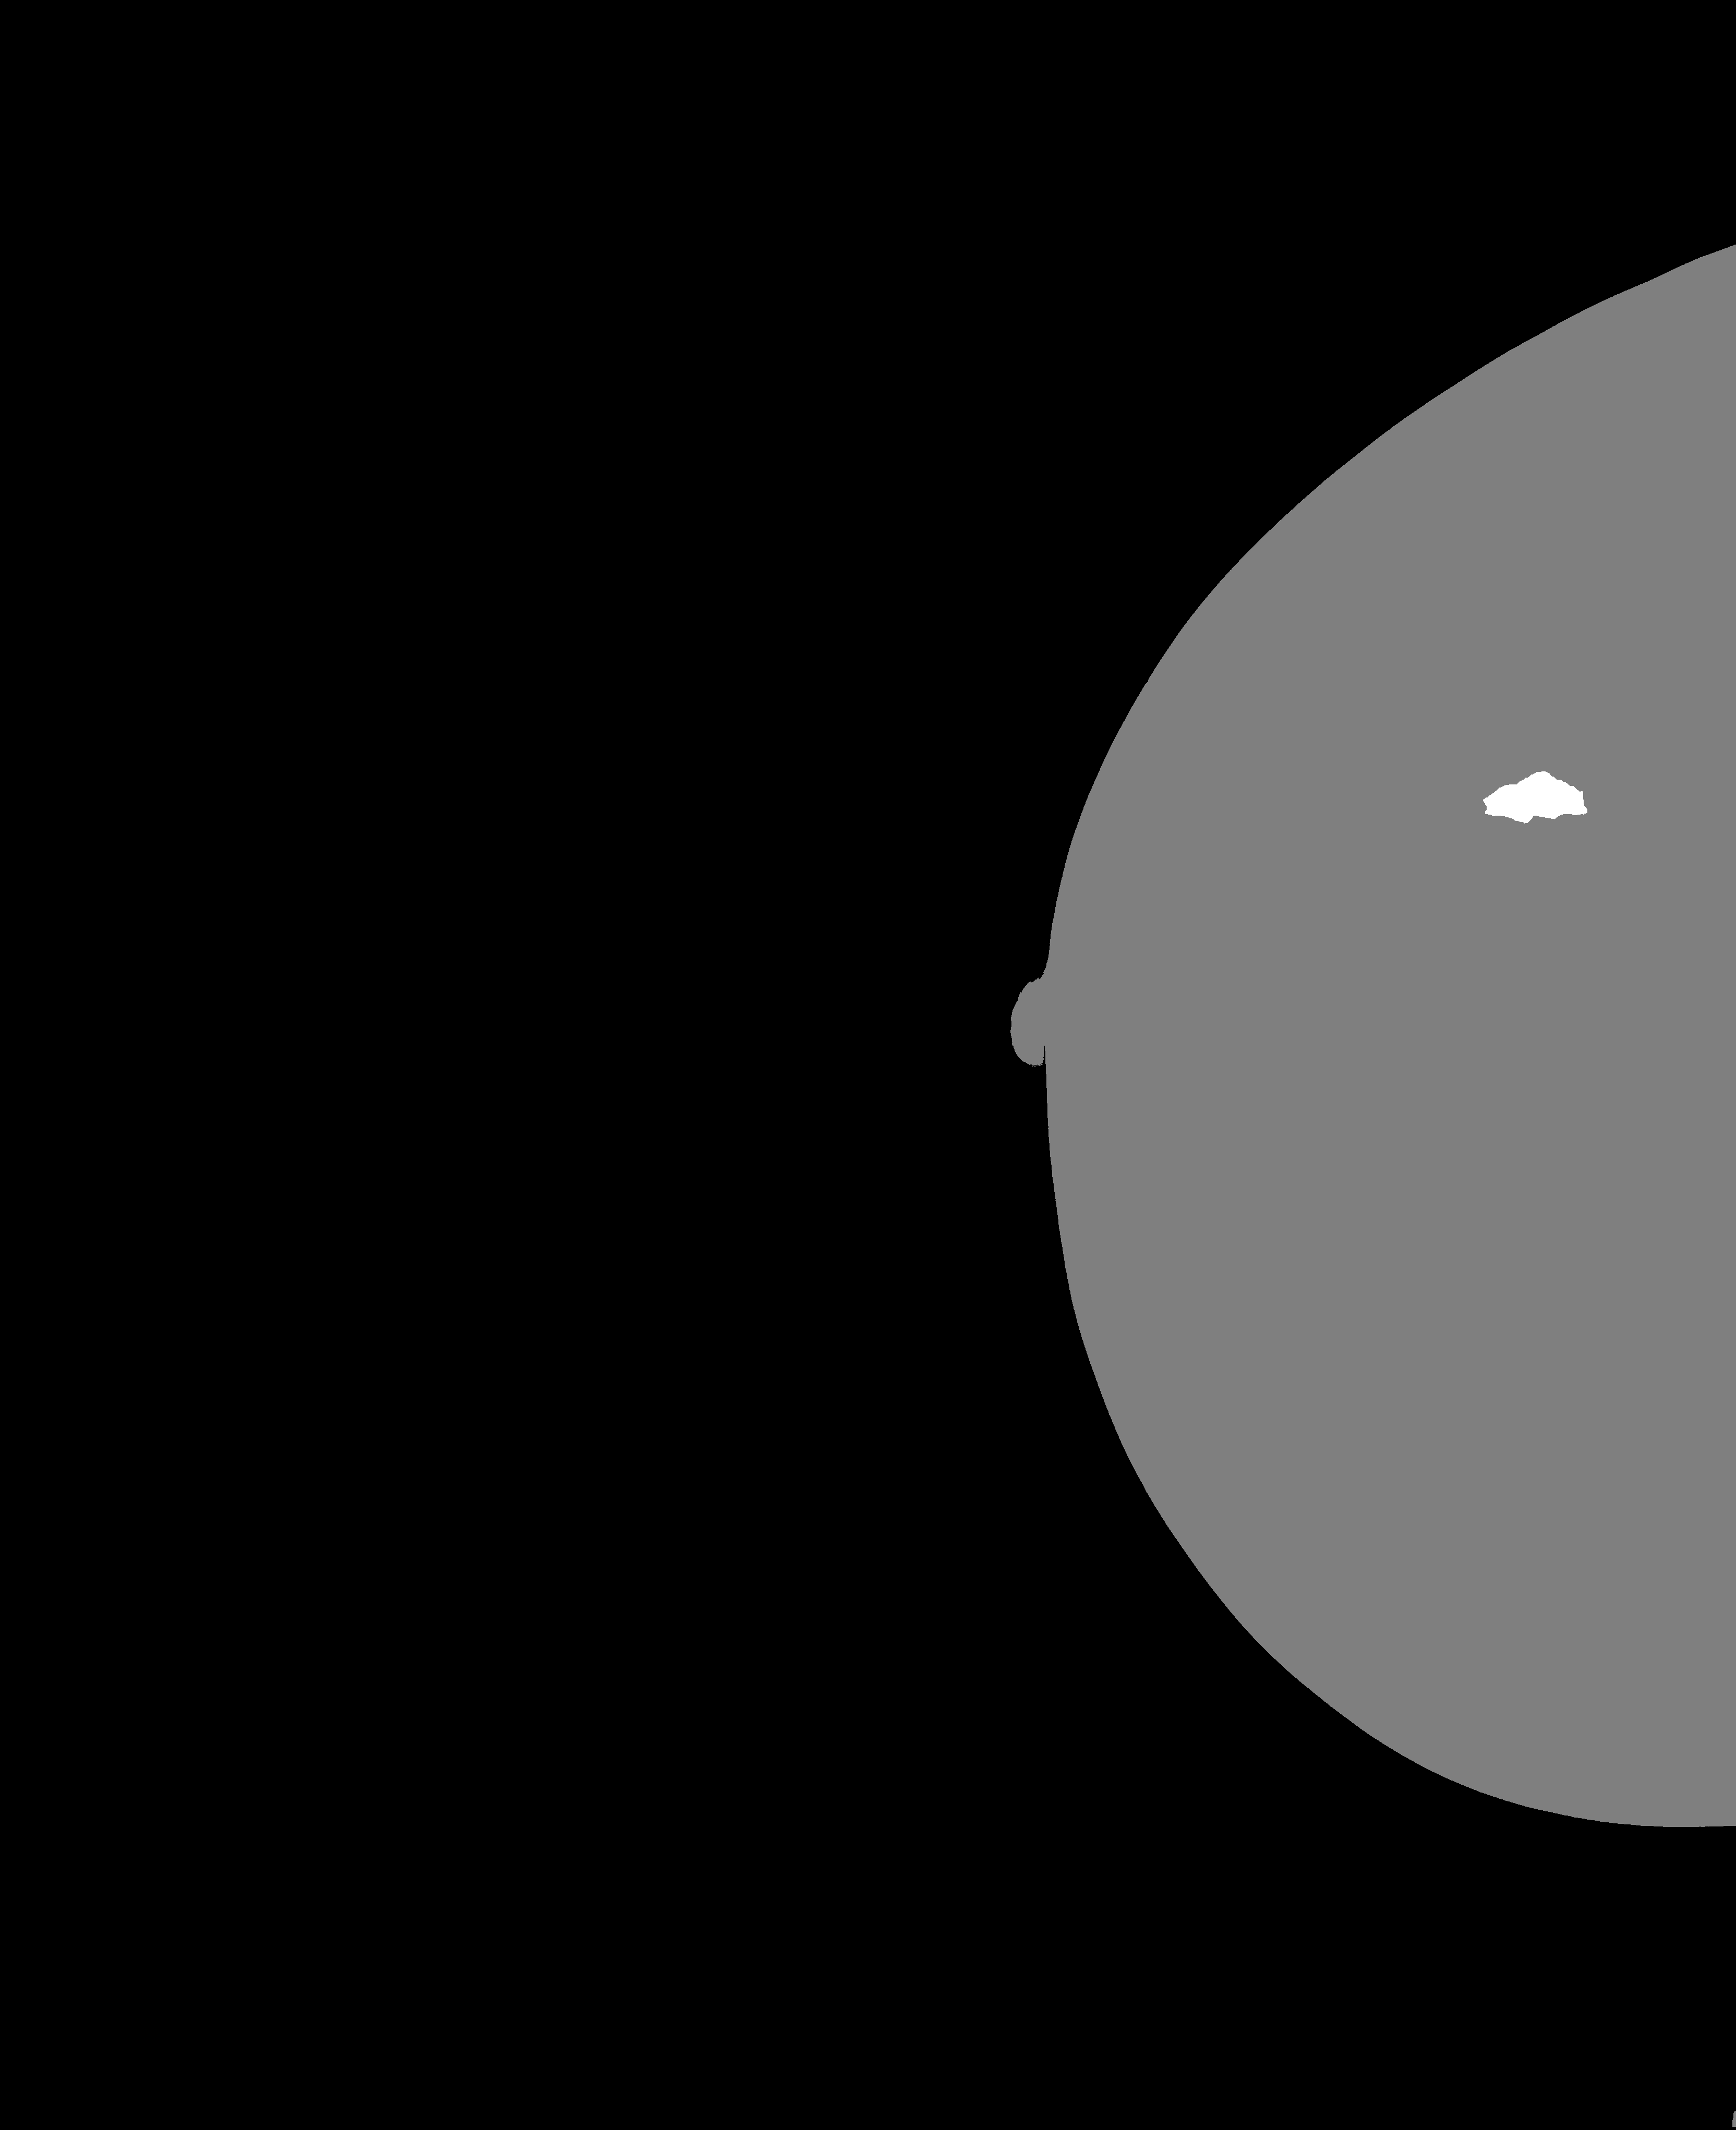
\includegraphics[height = 3.5cm]{plots/label_enhanced.png}
				\caption{Enhancement}
				\label{subfig:Preprocessingb}
			\end{subfigure}
			\begin{subfigure}{0.24\textwidth}
				\centering
					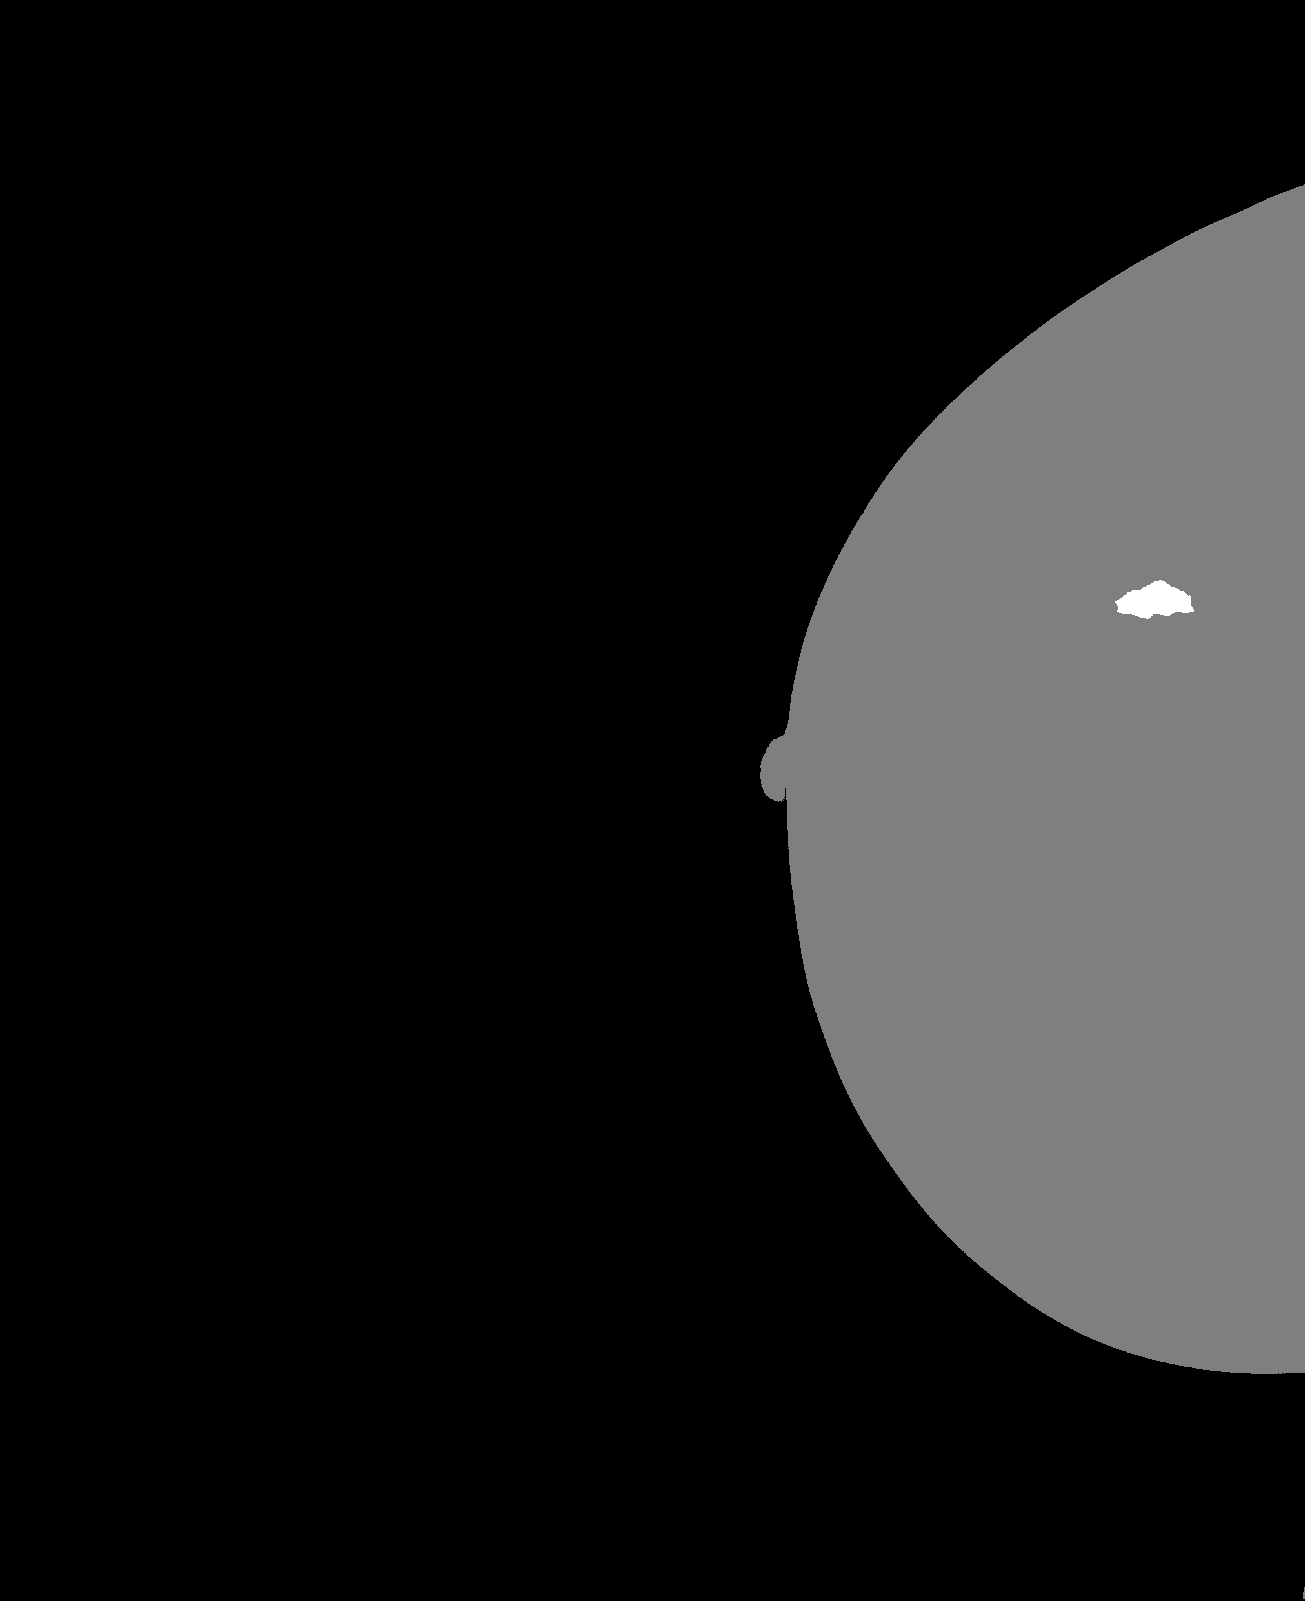
\includegraphics[height = 3.5cm]{plots/label_resized.png}
				\caption{Downsampling}
				\label{subfig:Preprocessingc}
			\end{subfigure}
			\begin{subfigure}{0.11\textwidth}
				\centering
					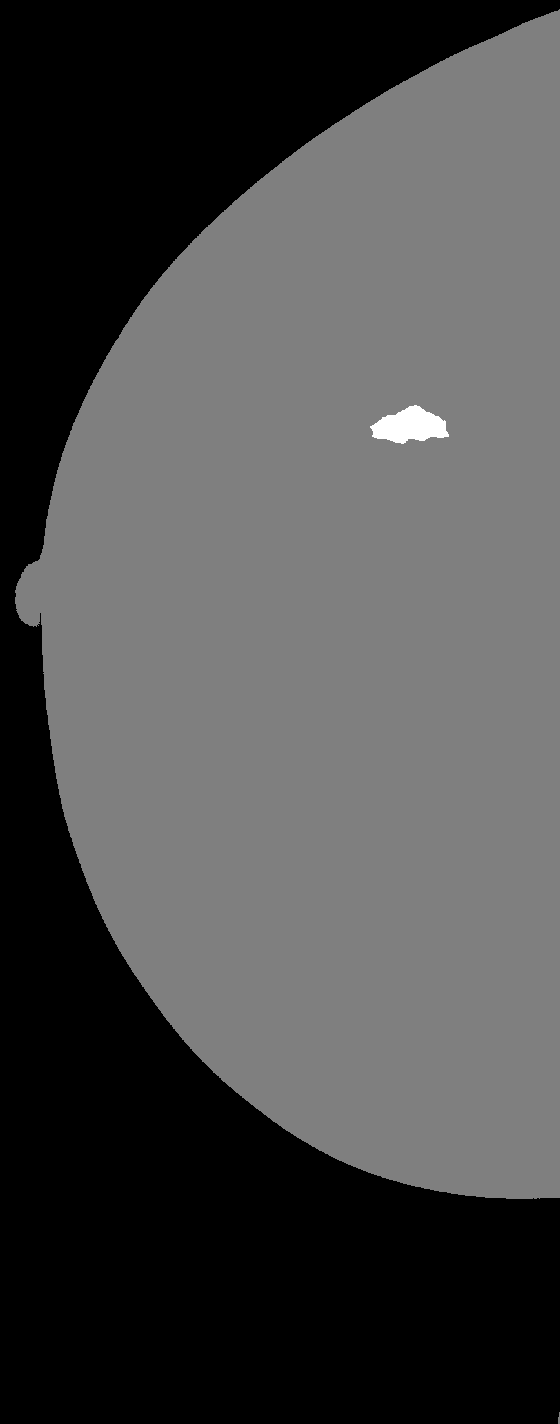
\includegraphics[height = 3.5cm]{plots/label_v1.png}
				\caption{Final}
				\label{subfig:Preprocessingd}
			\end{subfigure}
			% img_108_146_1_RCC.png
		\end{figure}
	\end{frame}
	
	\begin{frame}
		\frametitle{Software}
		\begin{figure}[h]
			\centering
			\begin{subfigure}{0.47\textwidth}
				\begin{subfigure}{\textwidth}
					
\includegraphics[width=\textwidth]{plots/tensorflow.png}
				\end{subfigure}
				\par \bigskip
				\begin{subfigure}{\textwidth}
					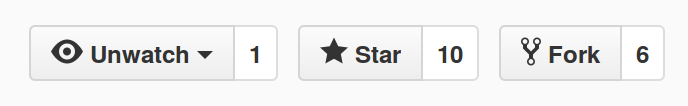
\includegraphics[width=\textwidth]{plots/github.png}
				\end{subfigure}
			\end{subfigure}
			~
			\begin{subfigure}{0.5\textwidth}
				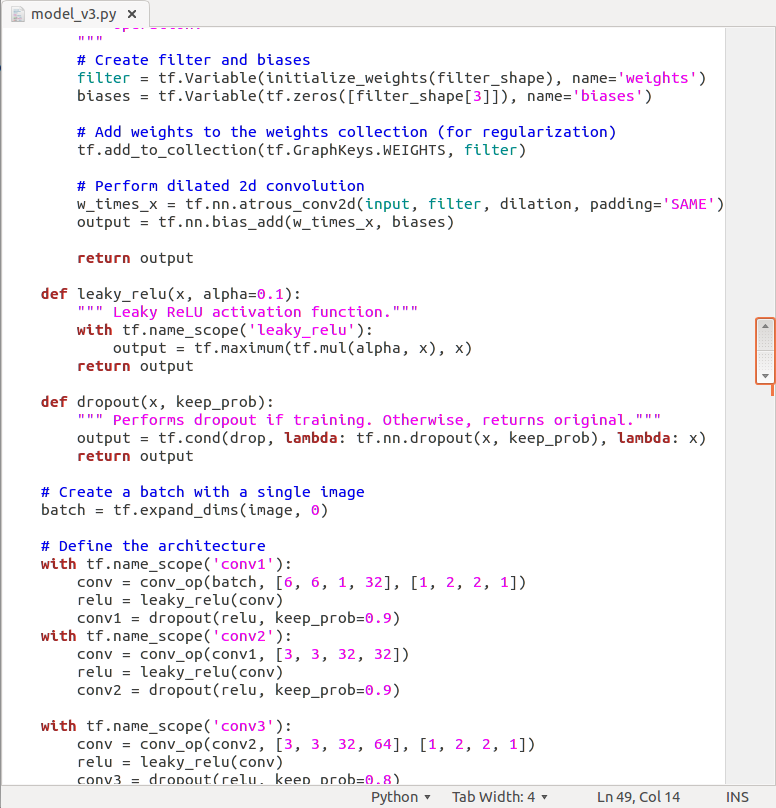
\includegraphics[width=\textwidth]{plots/code.png}
			\end{subfigure}
		\end{figure}
		%Seleccionar software, aprender tensorflow y havcer modelo.
	\end{frame}
	
	\begin{frame}
		\frametitle{Experiment 1}
		\footnotesize
		\begin{table}[h]
			\centering
			\begin{tabular}{lccccr}
			\hline
			\textbf{Layer} & \textbf{Filter} & \textbf{Stride} &\textbf{Pad} & \textbf{Volume} & \textbf{Parameters} \\
			\hline
			\texttt{INPUT}	& -	& - & - & $112 \times 112 \times 1$ & -\\
			\texttt{CONV -> Leaky RELU} & $6 \times 6$ & 2 & 2 & $56 \times 56 \times 56$ & 2\,072\\
			\texttt{CONV -> Leaky RELU} & $3 \times 3$ & 1 & 1 & $56 \times 56 \times 56$ & 28\,280\\
			\texttt{MAXPOOL} & $2 \times 2$ & 2 & 0 & $28 \times 28 \times 56$ & -\\
			\texttt{CONV -> Leaky RELU} & $3 \times 3$ & 1 & 1 & $28 \times 28 \times 84$ & 42\,420\\
			\texttt{CONV -> Leaky RELU} & $3 \times 3$ & 1 & 1 & $28 \times 28 \times 84$ & 63\,588\\
			\texttt{MAXPOOL} & $2 \times 2$ & 2 & 0 & $14 \times 14 \times 84$ & -\\
			\texttt{CONV -> Leaky RELU} & $3 \times 3$ & 1 & 1 & $14 \times 14 \times 112$ & 84\,784\\
			\texttt{CONV -> Leaky RELU} & $3 \times 3$ & 1 & 1 & $14 \times 14 \times 112$ & 113\,008\\
			\texttt{CONV -> Leaky RELU} & $3 \times 3$ & 1 & 1 & $14 \times 14 \times 112$ & 113\,008\\
			\texttt{MAXPOOL} & $2 \times 2$ & 2 & 0 & $7 \times 7 \times 112$ & -\\
			\texttt{FC -> Leaky RELU} & $7 \times 7$ & 1 & 3 & $7 \times 7 \times 448$ & 2\,459\,072\\
			\texttt{FC} & $1 \times 1$ & 1 & 0 & $7 \times 7 \times 1$ & 449 \\
			\texttt{BILINEAR (x16)} & - & - & - & $112 \times 112 \times 1$ & -\\
			\hline
			\end{tabular}
		\end{table}
		
		\scriptsize
		\begin{table}[h]
			\centering
			\begin{tabular}{cccccccc}
			\hline
			\textbf{IOU}	& \textbf{F1-score}	& \textbf{G-mean} &\textbf{Accuracy}	& \textbf{Sensitivity} & \textbf{Specificity} & \textbf{Precision} & \textbf{Recall}\\
			\hline
			0.022 & 0.031 & 0.038 & 0.975 & 0.028 & 0.982 & 0.040 & 0.028\\
			\hline
			\end{tabular}
		\end{table}

	\end{frame}
	
	\begin{frame}
		\frametitle{Qualitative results}
		\begin{figure}[h]
		\centering
			\begin{subfigure}{0.25\textwidth}
				\centering
					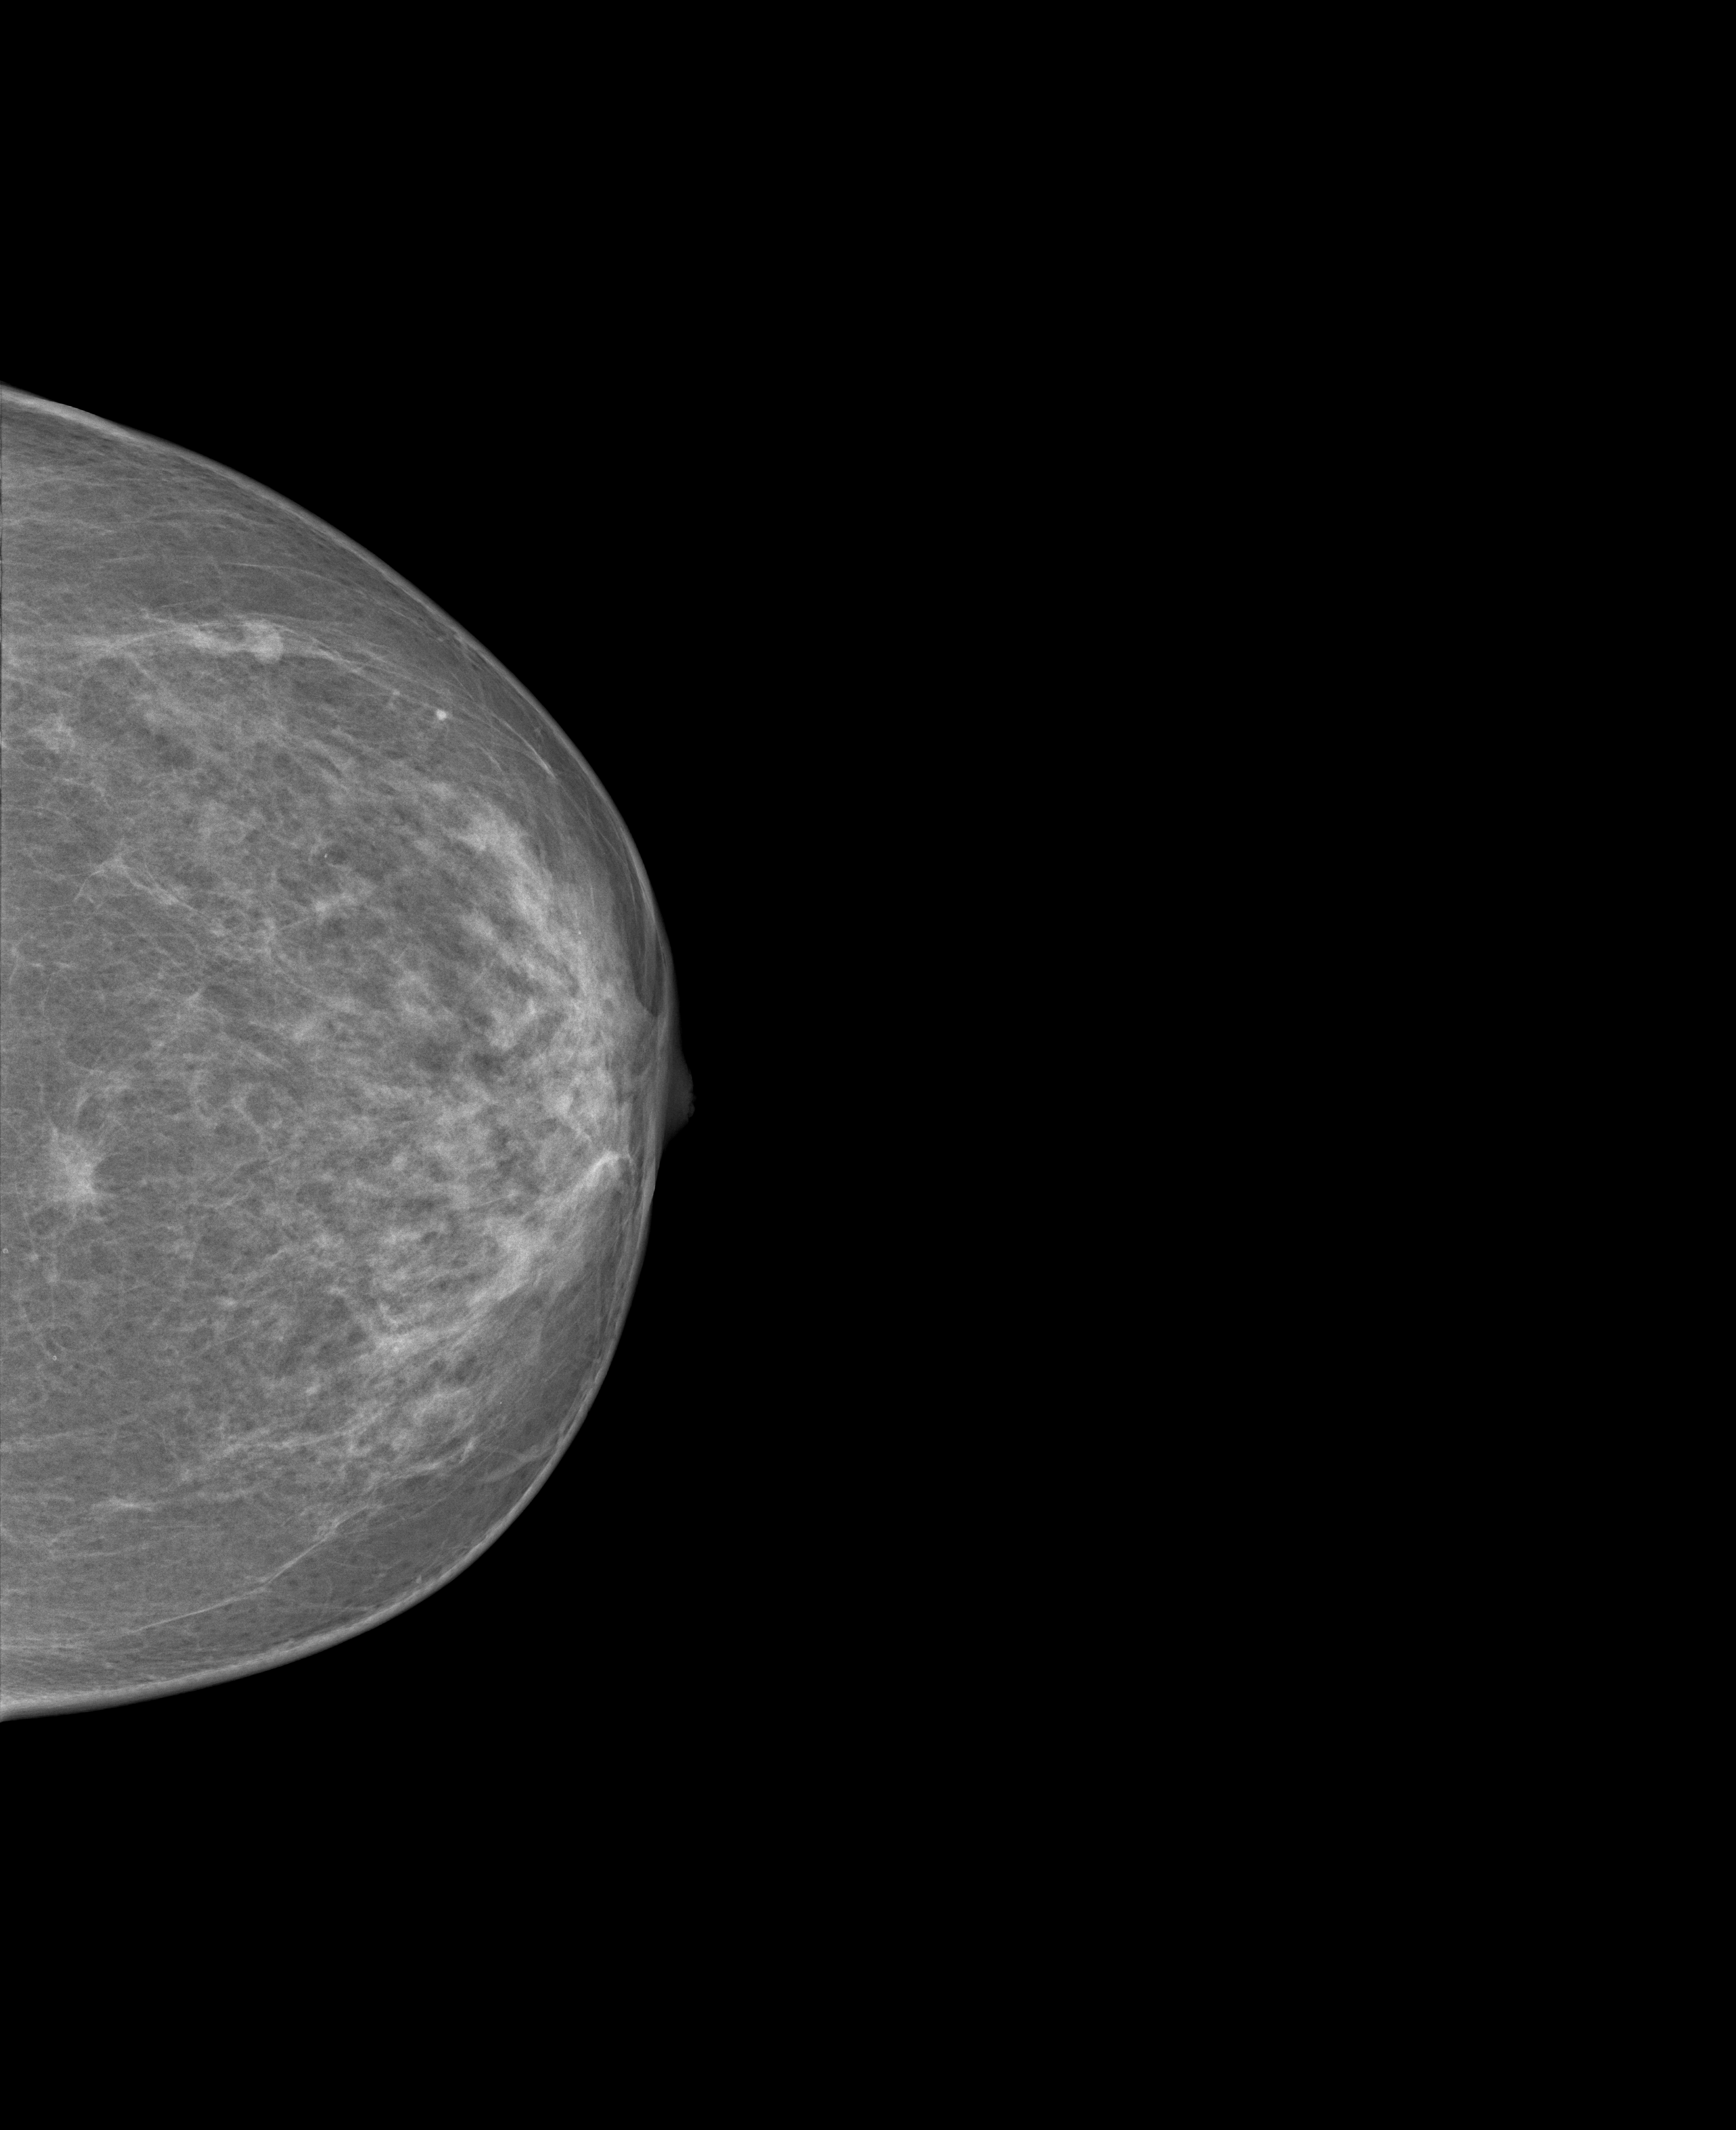
\includegraphics[height=3.5cm]{plots/mammogram_ex1.png}
			\end{subfigure}
			\begin{subfigure}{0.16\textwidth}
				\centering
					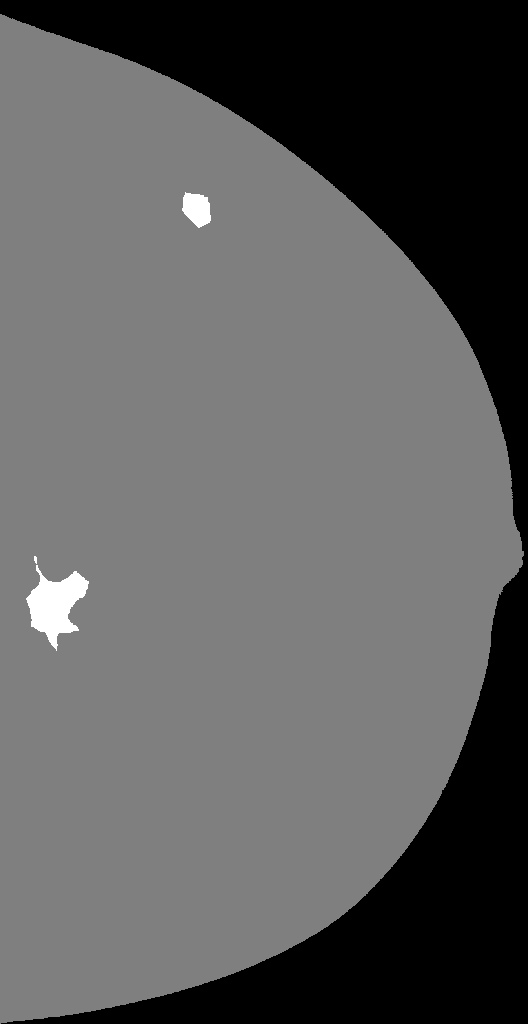
\includegraphics[height=3.5cm]{plots/label_ex1.png}
			\end{subfigure}
			\begin{subfigure}{0.17\textwidth}
				\centering
					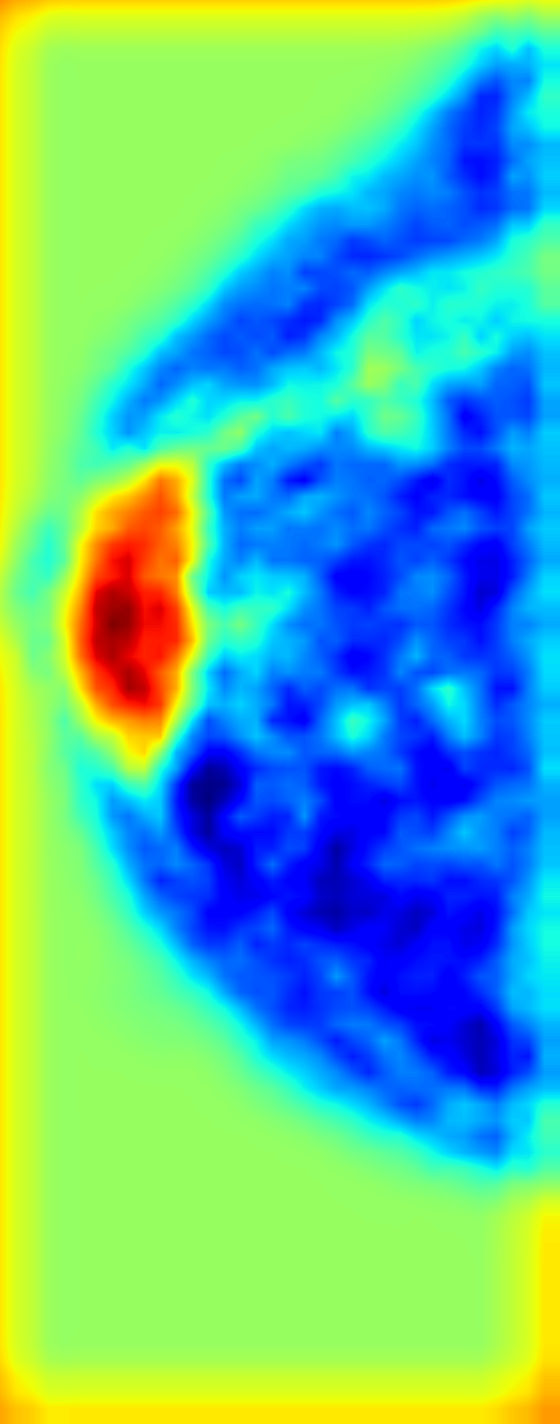
\includegraphics[height=3.5cm]{plots/logits_ex1_v1.png}
			\end{subfigure}
			\begin{subfigure}{0.22\textwidth}
				\centering
					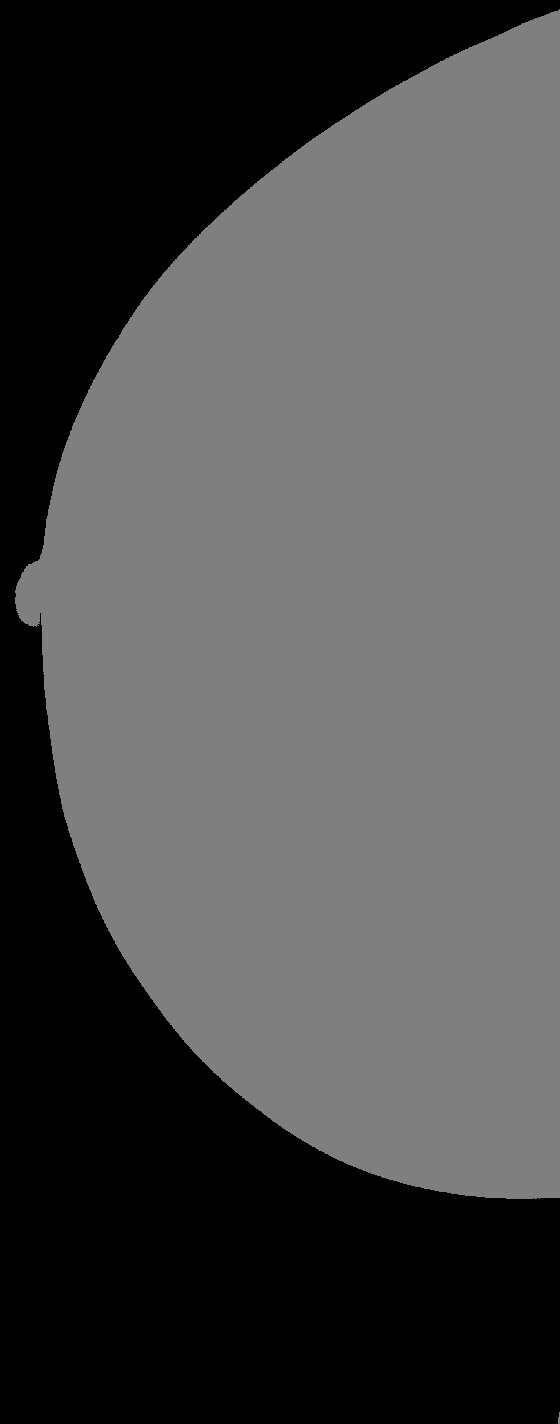
\includegraphics[height=3.5cm]{plots/segmentation_ex1_v1.png}
			\end{subfigure}% img_108_146_1_RCC.png
			\\
			\begin{subfigure}{0.25\textwidth}
				\centering
					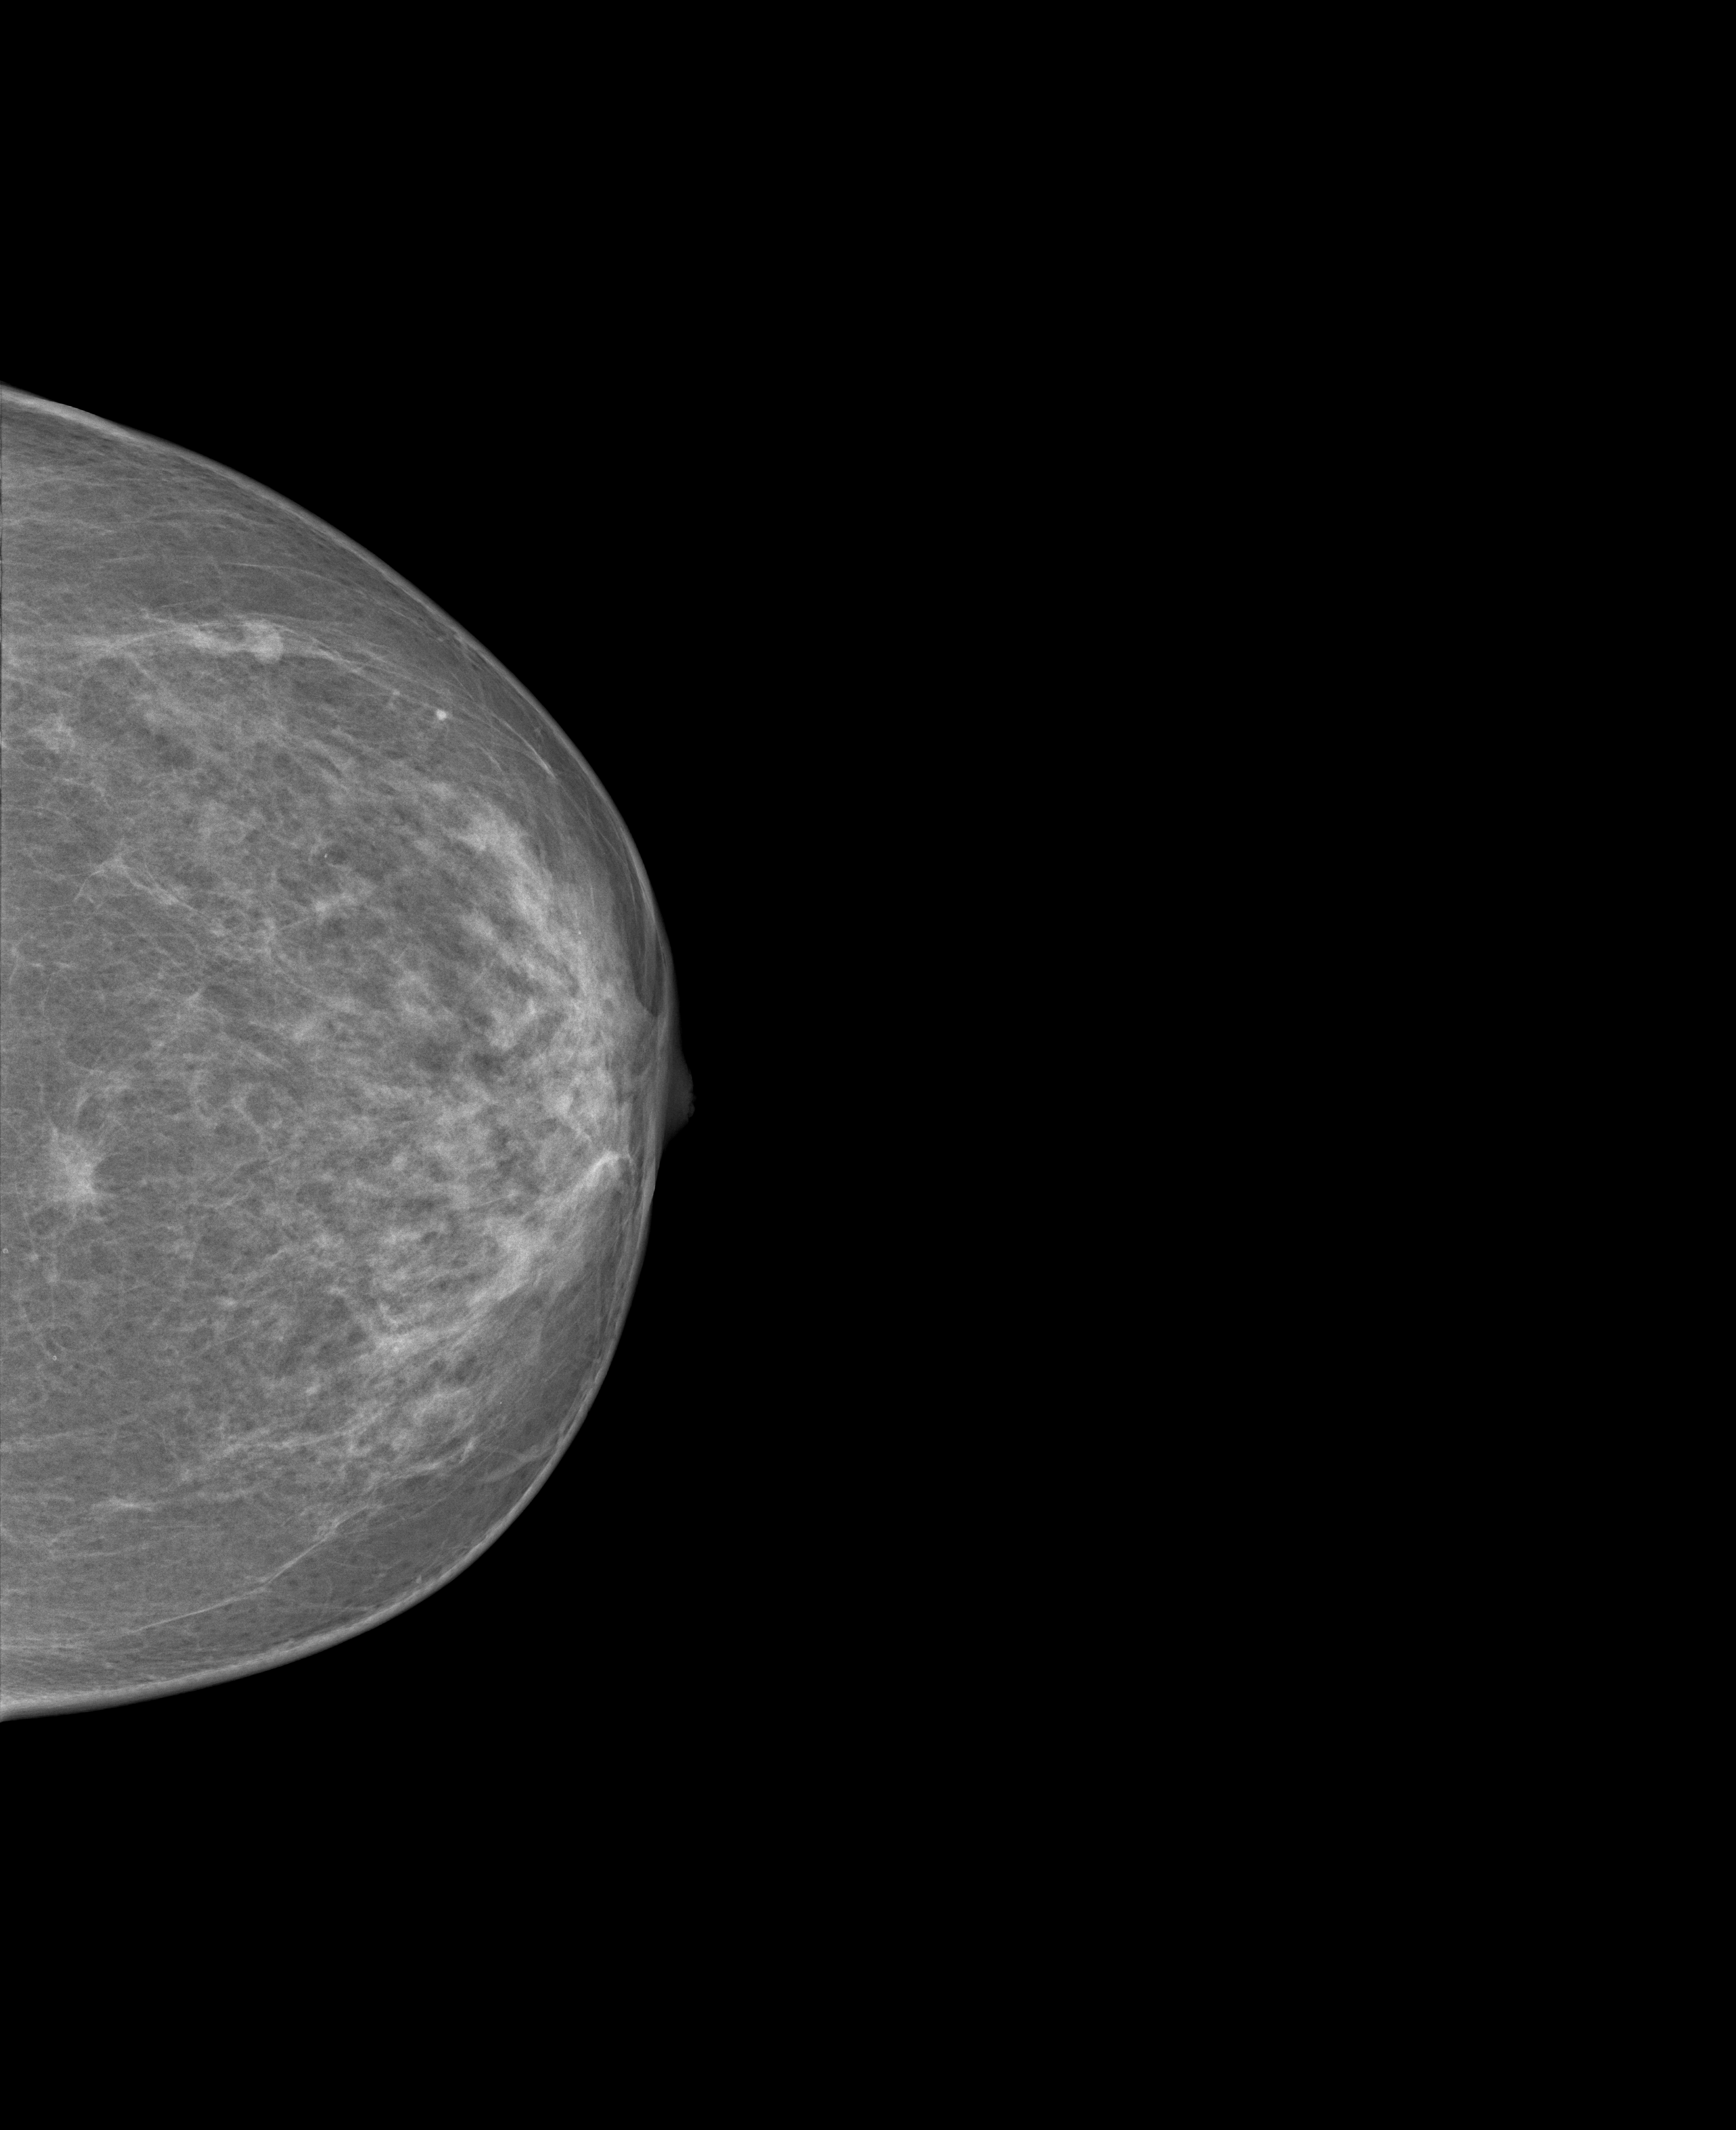
\includegraphics[height = 3.5cm]{plots/mammogram_ex2.png}
				\caption{Original}
			\end{subfigure}
			\begin{subfigure}{0.16\textwidth}
				\centering
					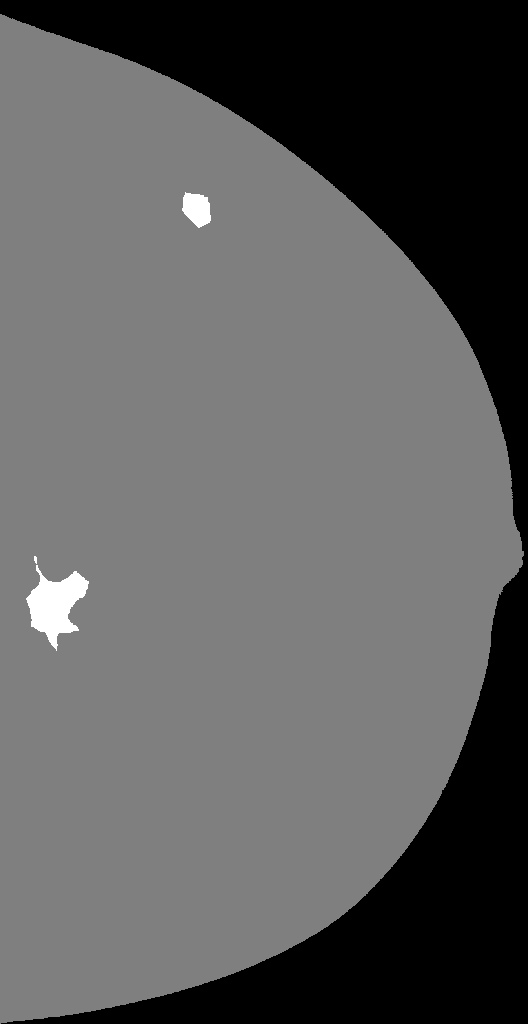
\includegraphics[height = 3.5cm]{plots/label_ex2.png}
				\caption{Label}
			\end{subfigure}
			\begin{subfigure}{0.17\textwidth}
				\centering
					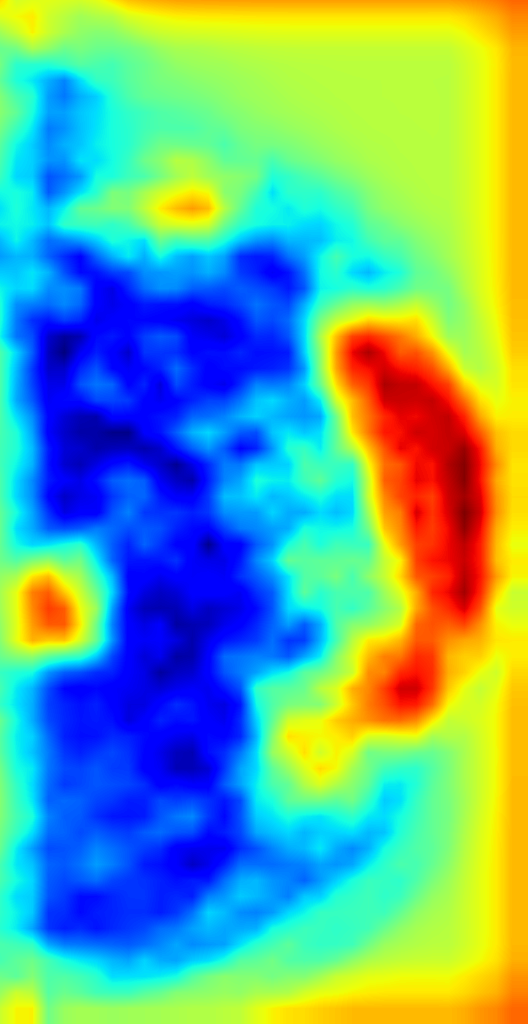
\includegraphics[height = 3.5cm]{plots/logits_ex2_v1.png}
				\caption{Prediction}
			\end{subfigure}
			\begin{subfigure}{0.22\textwidth}
				\centering
					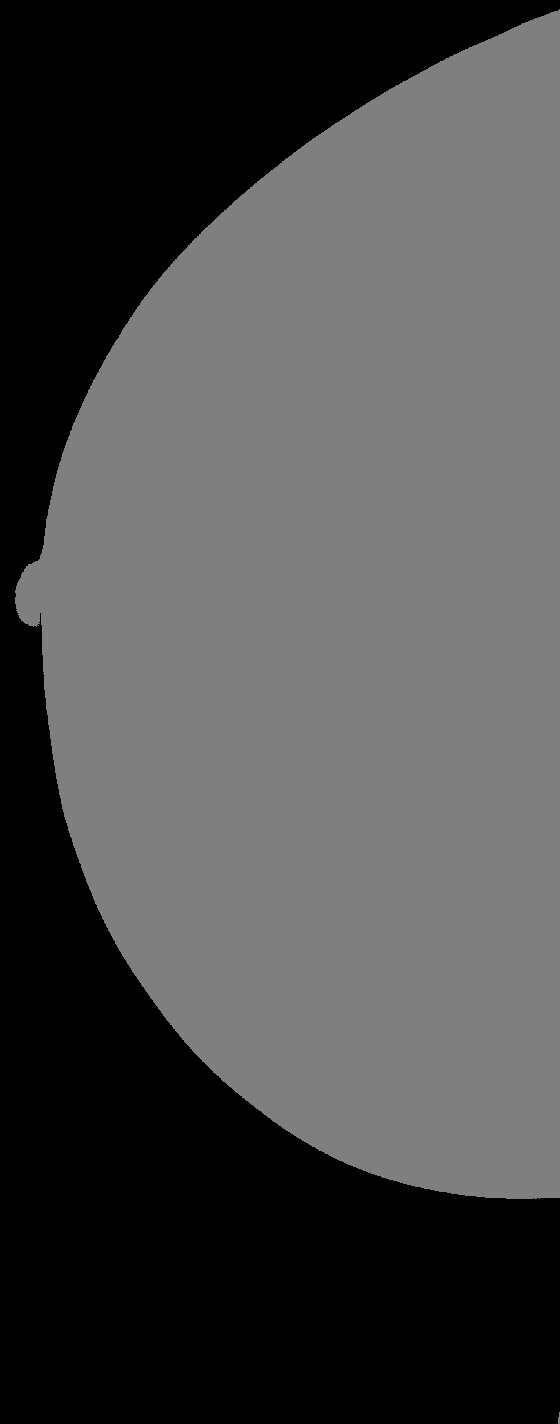
\includegraphics[height = 3.5cm]{plots/segmentation_ex2_v1.png}
				\caption{Segmentation}
			\end{subfigure}%img_251_334_1_LCC.png
		\end{figure}		
	\end{frame}
	
	\begin{frame}
		\frametitle{Experiment 2}
		Weighted loss function.
		
		\scriptsize
		\begin{table}[h]
			\centering
			\begin{tabular}{cccccccc}
			\hline
			\textbf{IOU}	& \textbf{F1-score}	& \textbf{G-mean} &\textbf{Accuracy}	& \textbf{Sensitivity} & \textbf{Specificity} & \textbf{Precision} & \textbf{Recall}\\
			\hline
			 0.028 & 0.041 & 0.071 & 0.967 & 0.046 & 0.973 & 0.052 & 0.046\\
			\hline
			\end{tabular}
		\end{table}
	\end{frame}
	
	\begin{frame}
		\frametitle{Qualitative results}
		\begin{figure}[h]
		\centering
			\begin{subfigure}{0.25\textwidth}
				\centering
					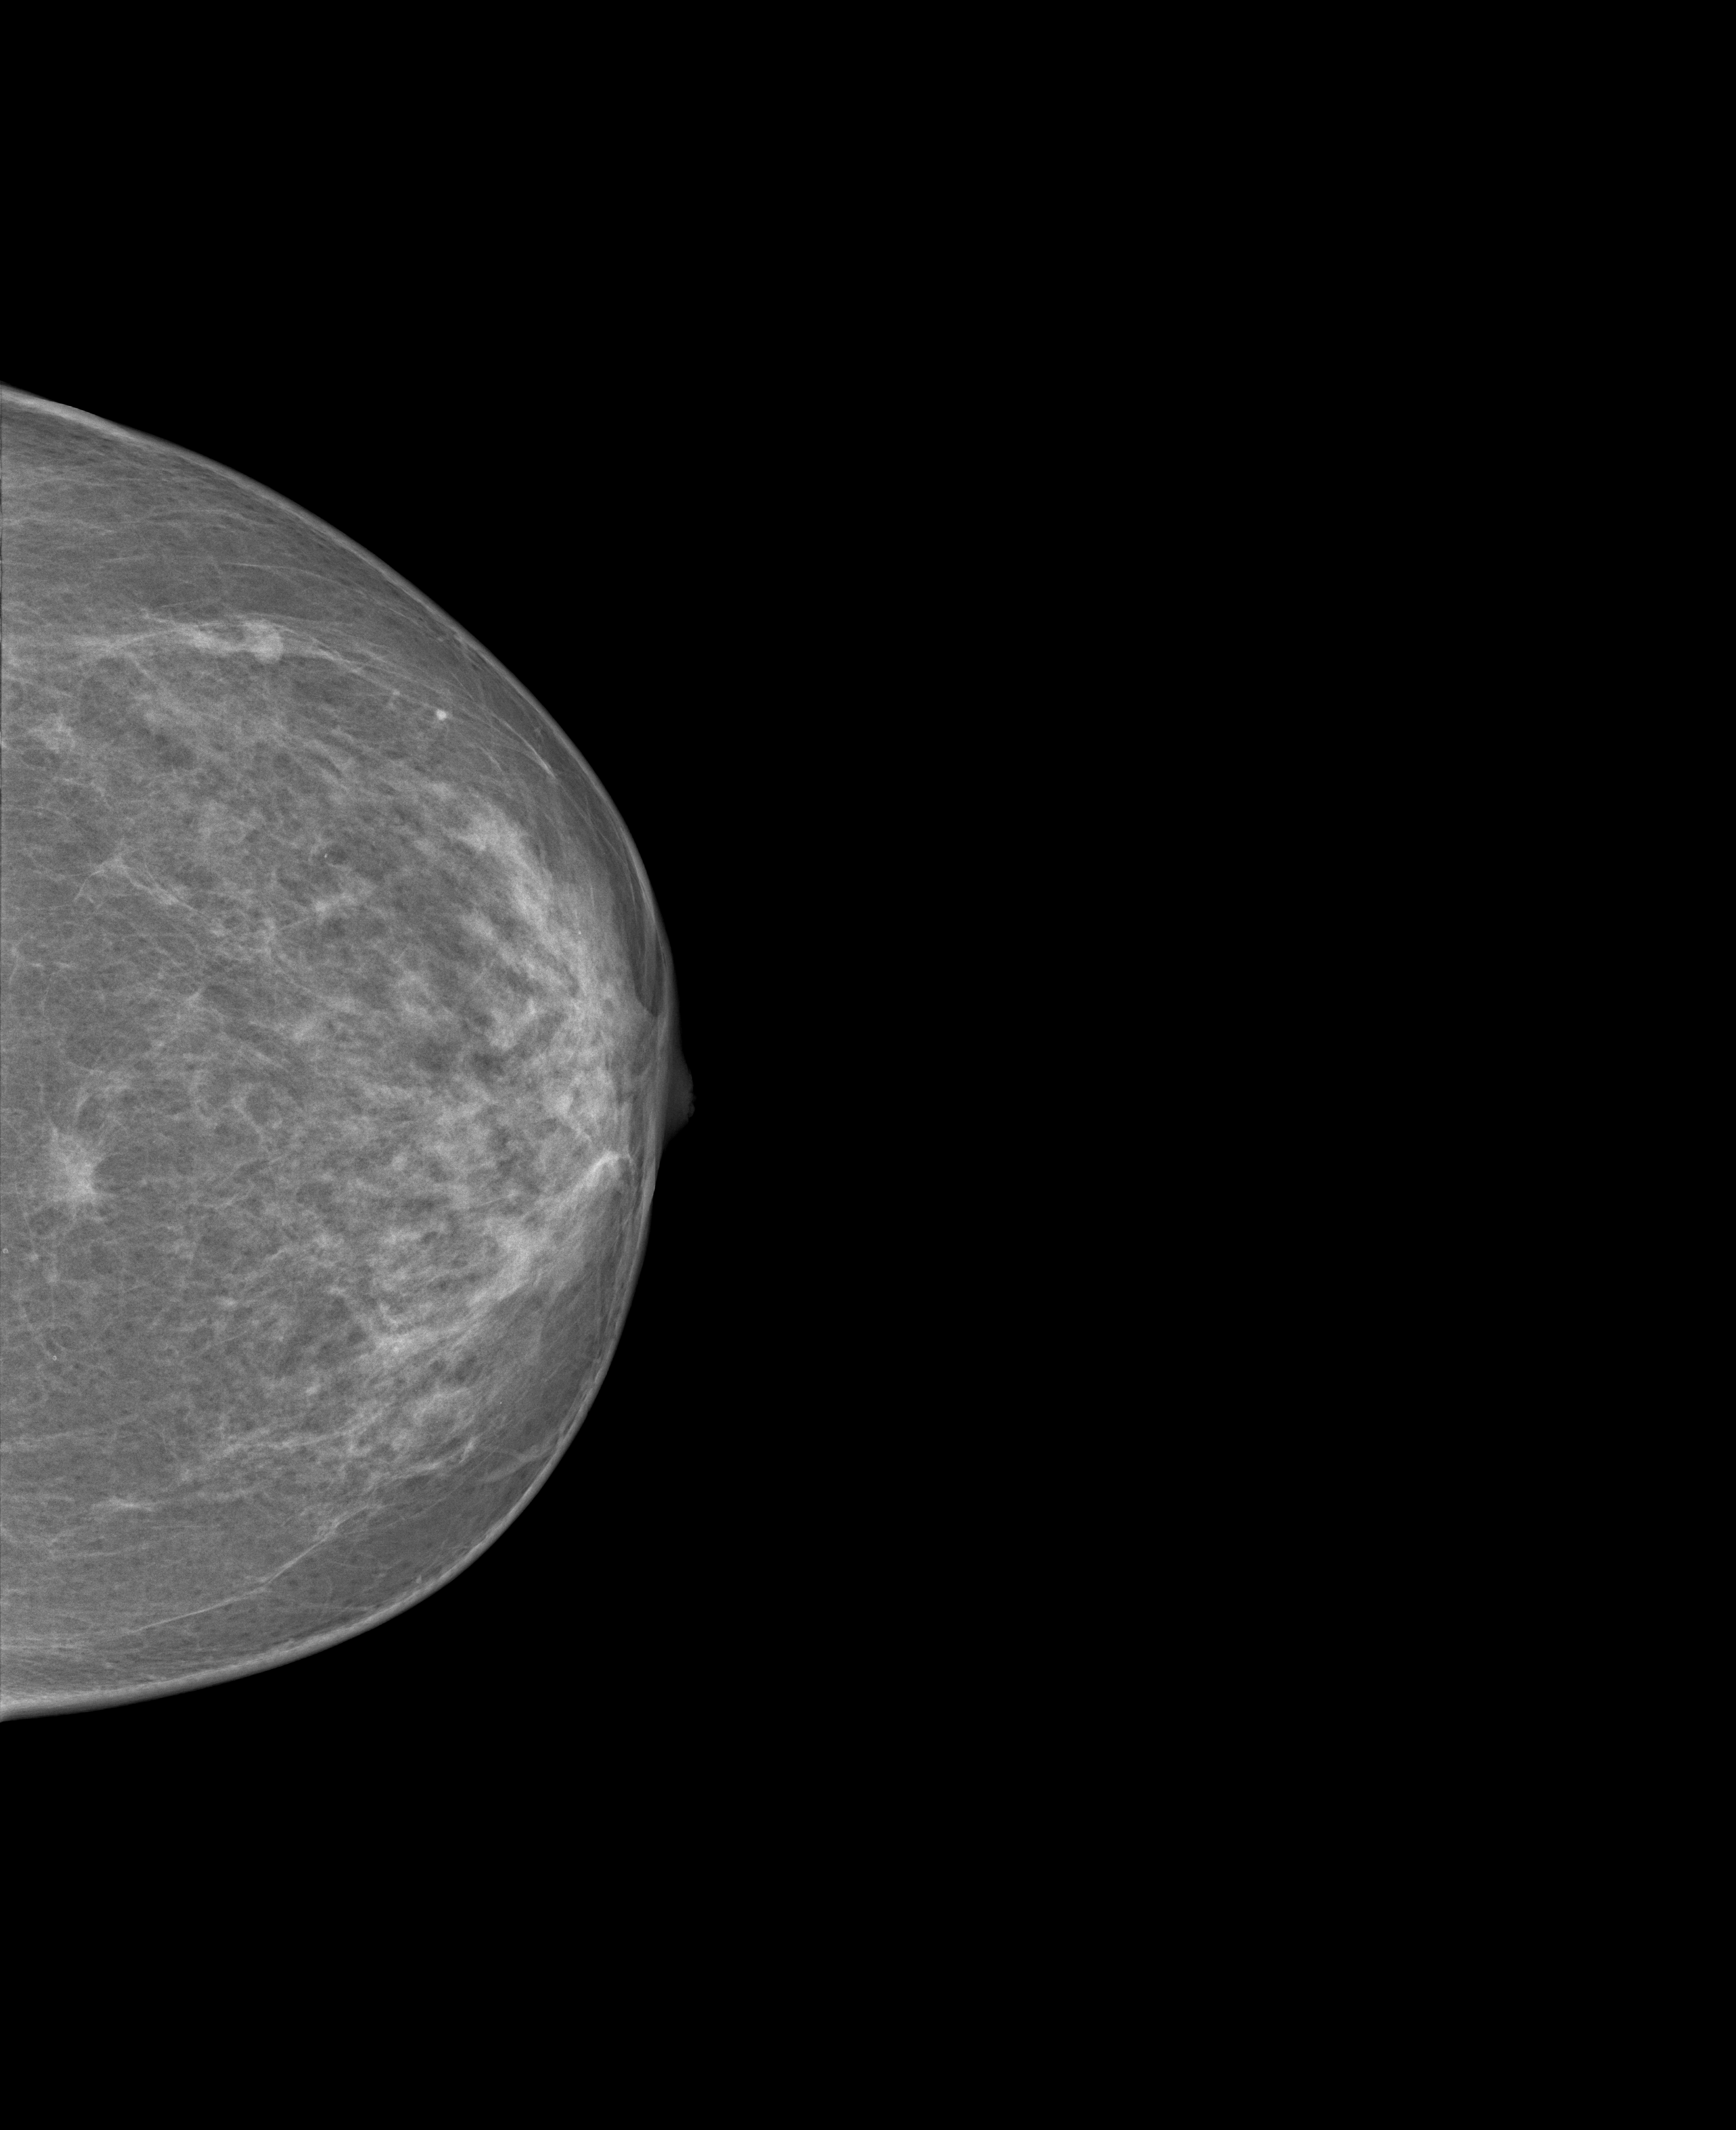
\includegraphics[height=3.5cm]{plots/mammogram_ex1.png}
			\end{subfigure}
			\begin{subfigure}{0.16\textwidth}
				\centering
					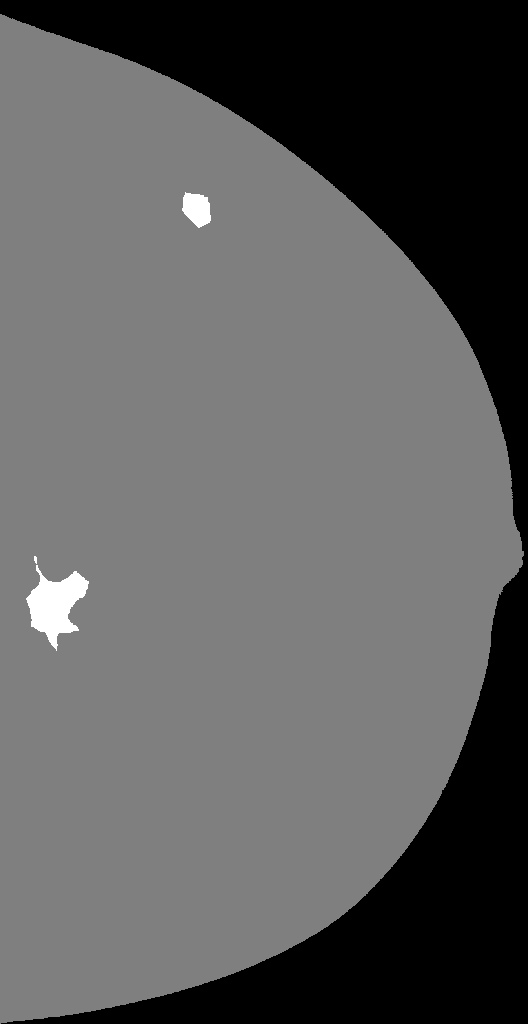
\includegraphics[height=3.5cm]{plots/label_ex1.png}
			\end{subfigure}
			\begin{subfigure}{0.17\textwidth}
				\centering
					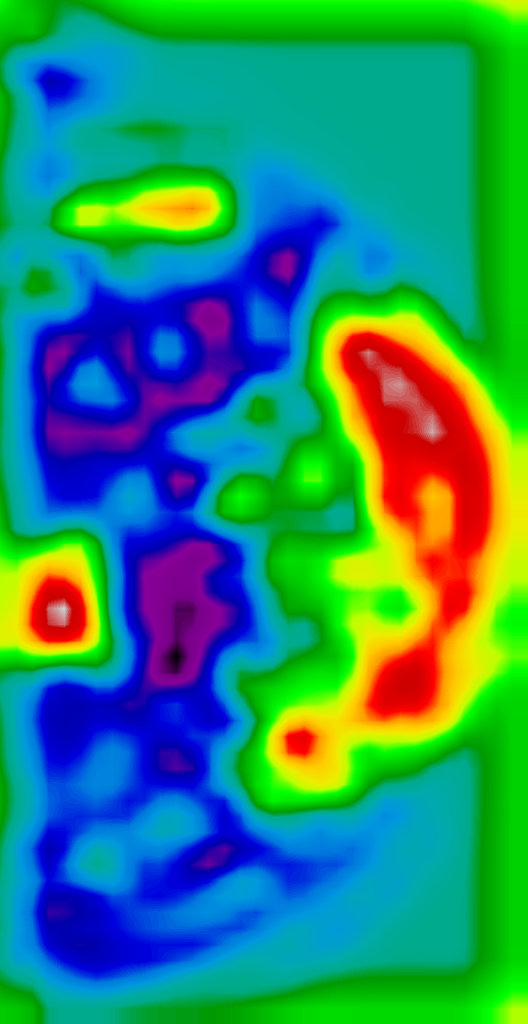
\includegraphics[height=3.5cm]{plots/logits_ex1_v2.png}
			\end{subfigure}
			\begin{subfigure}{0.22\textwidth}
				\centering
					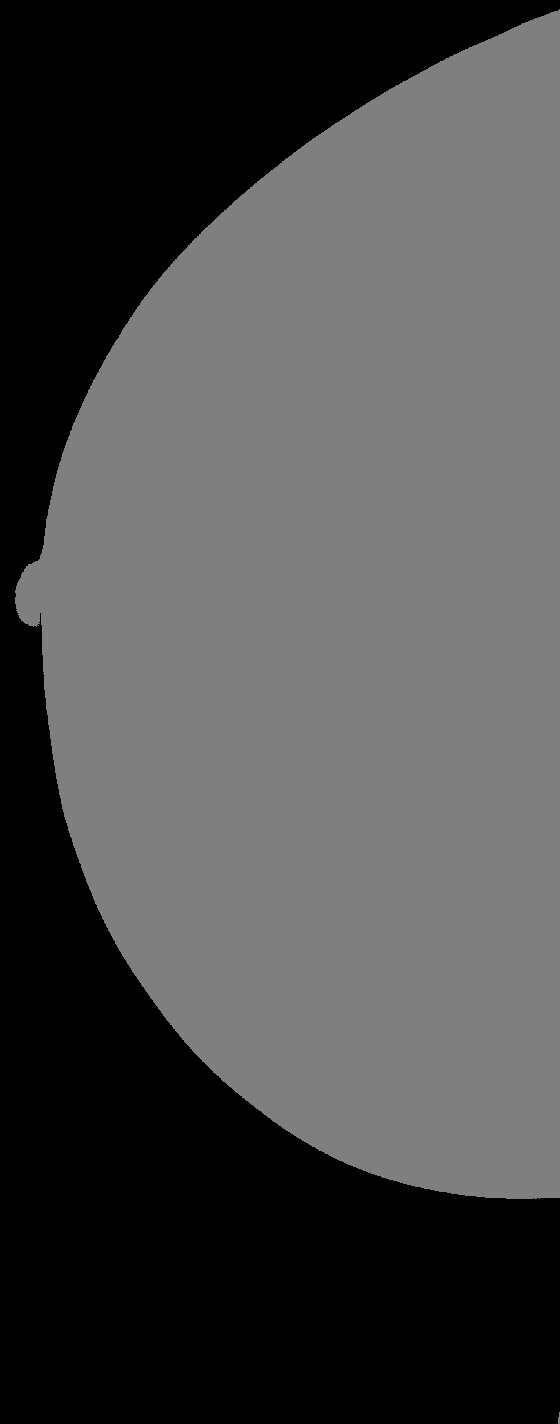
\includegraphics[height=3.5cm]{plots/segmentation_ex1_v2.png}
			\end{subfigure}% img_108_146_1_RCC.png
			\\
			\begin{subfigure}{0.25\textwidth}
				\centering
					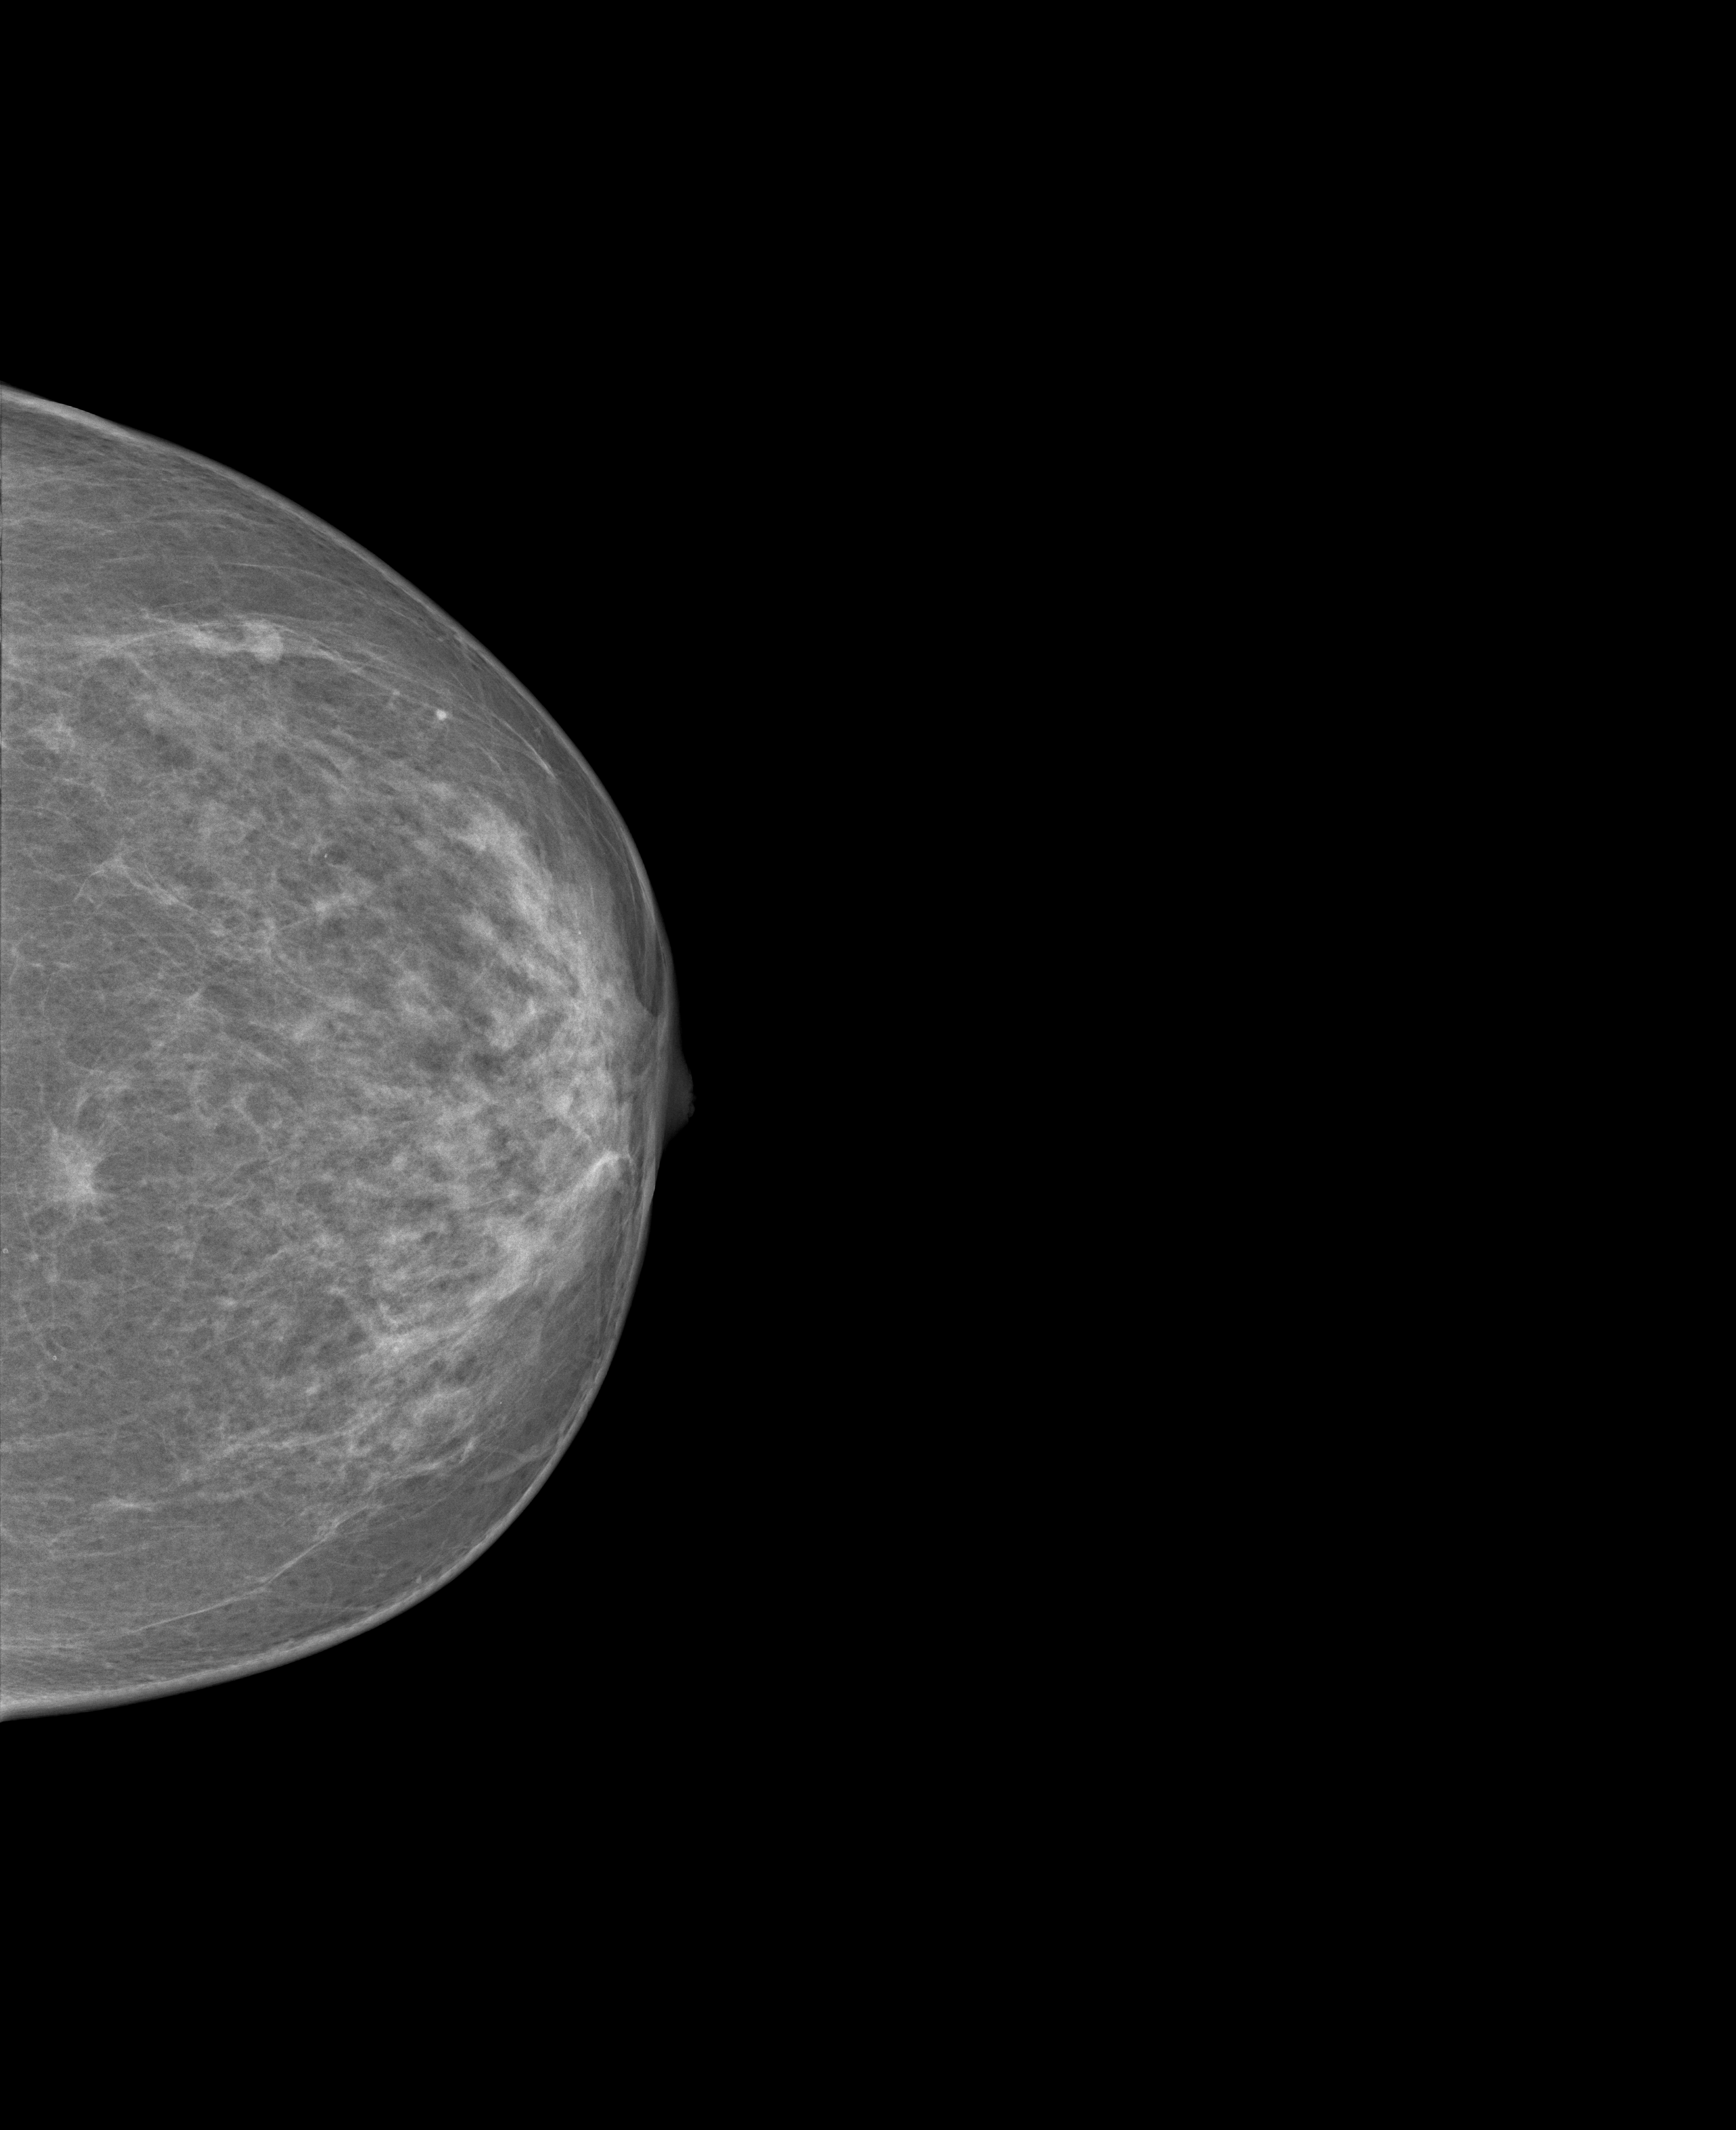
\includegraphics[height = 3.5cm]{plots/mammogram_ex2.png}
				\caption{Original}
			\end{subfigure}
			\begin{subfigure}{0.16\textwidth}
				\centering
					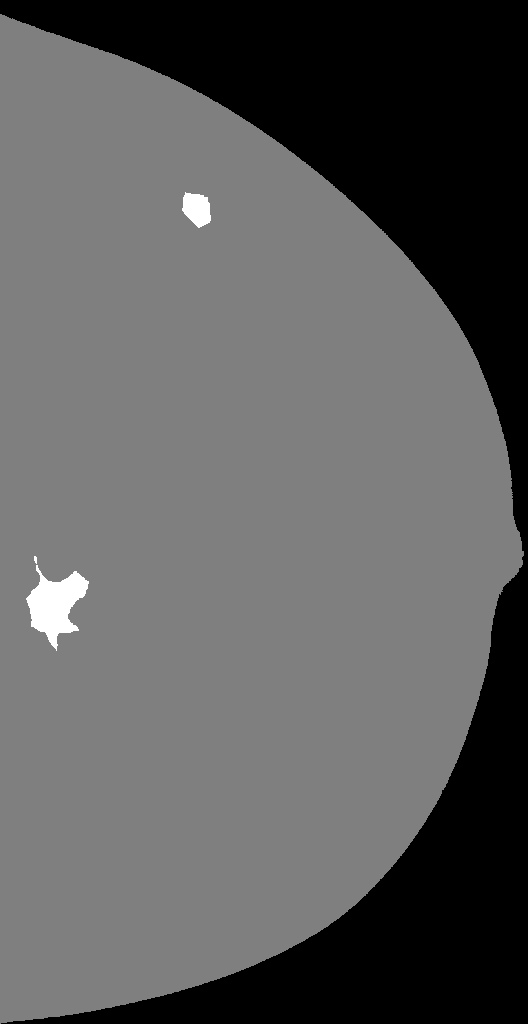
\includegraphics[height = 3.5cm]{plots/label_ex2.png}
				\caption{Label}
			\end{subfigure}
			\begin{subfigure}{0.17\textwidth}
				\centering
					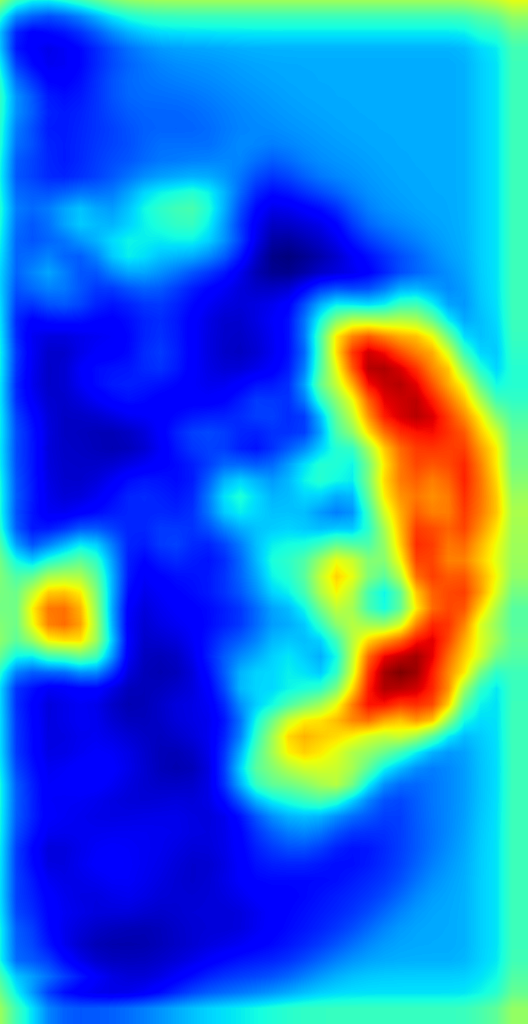
\includegraphics[height = 3.5cm]{plots/logits_ex2_v2.png}
				\caption{Prediction}
			\end{subfigure}
			\begin{subfigure}{0.22\textwidth}
				\centering
					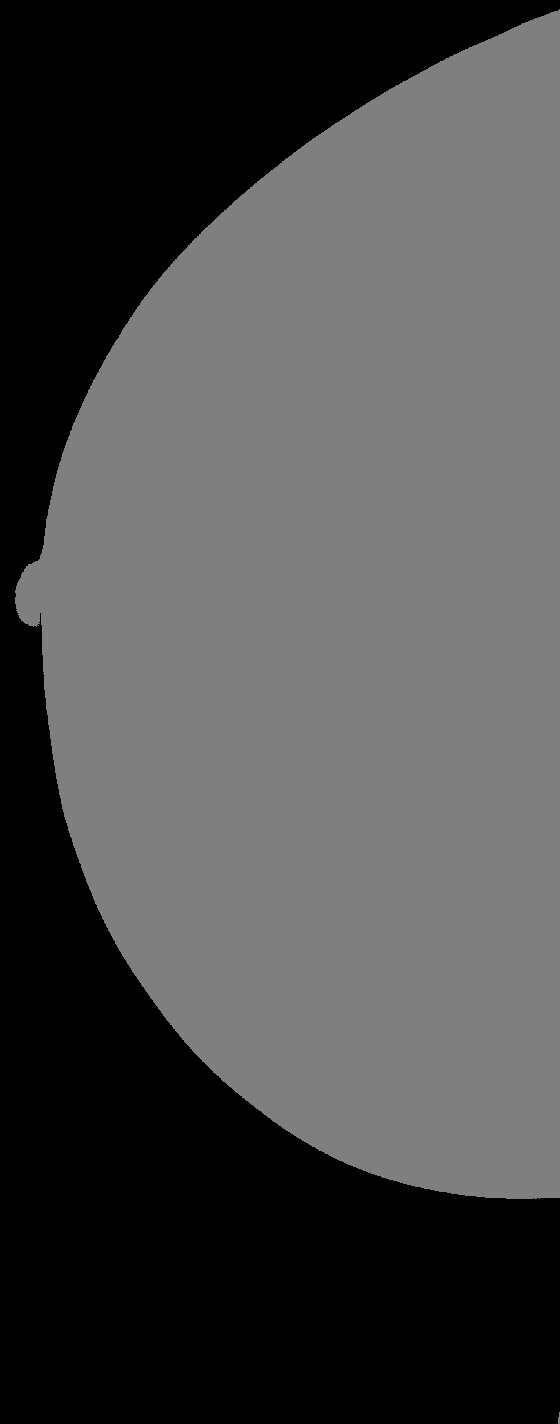
\includegraphics[height = 3.5cm]{plots/segmentation_ex2_v2.png}
				\caption{Segmentation}
			\end{subfigure}%img_251_334_1_LCC.png
		\end{figure}		
	\end{frame}
	
	\begin{frame}
		\frametitle{Experiment 3}
		\footnotesize
		\begin{table}[h]
			\centering
			\begin{tabular}{lcccccr}
			\hline
			\textbf{Layer} & \textbf{Filter} & \textbf{Stride} & \textbf{Pad} & \textbf{Dilation} & \textbf{Volume} & \textbf{Parameters} \\
			\hline
			\texttt{INPUT}	&- & -	& - & - & $128 \times 128 \times 1$ & -\\
			\texttt{CONV -> LRELU}	& $6 \times 6$ & 2 & 2 & 1 & $64 \times 64 \times 32$ & 1\,184\\
			\texttt{CONV -> LRELU}	& $3 \times 3$ & 1 & 1 & 1 & $64 \times 64 \times 32$ & 9\,248\\
			\texttt{CONV -> LRELU}	& $3 \times 3$ & 2 & 1 & 1 & $32 \times 32 \times 64$ & 18\,496\\
			\texttt{CONV -> LRELU}	& $3 \times 3$ & 1 & 1 & 1 & $32 \times 32 \times 64$ & 36\,928\\
			\texttt{CONV -> LRELU}	& $3 \times 3$ & 1 & 2 & 2 & $32 \times 32 \times 128$ & 73\,856\\
			\texttt{CONV -> LRELU}	& $3 \times 3$ & 1 & 2 & 2 & $32 \times 32 \times 128$ & 147\,584\\
			\texttt{CONV -> LRELU}	& $3 \times 3$ & 1 & 2 & 2 & $32 \times 32 \times 128$ & 147\,584\\
			\texttt{CONV -> LRELU}	& $3 \times 3$ & 1 & 2 & 2 & $32 \times 32 \times 128$ & 147\,584\\
			\texttt{CONV -> LRELU}	& $3 \times 3$ & 1 & 4 & 4 & $32 \times 32 \times 256$ & 295\,168\\
			\texttt{CONV}	& $8 \times 8$ & 1 & 14 & 4 & $32 \times 32 \times 1$ & 16\,385\\
			\texttt{BILINEAR (x4)}		& - & - && - & $128 \times 128 \times 1$ & -\\
			\hline
			\end{tabular}
		\end{table}
		
		\scriptsize
		\begin{table}[h]
			\centering
			\begin{tabular}{cccccccc}
			\hline
			\textbf{IOU}	& \textbf{F1-score}	& \textbf{G-mean} &\textbf{Accuracy}	& \textbf{Sensitivity} & \textbf{Specificity} & \textbf{Precision} & \textbf{Recall}\\
			\hline
			 - & - & - & - & - & - & - & -\\
			\hline
			\end{tabular}
		\end{table}
	\end{frame}
	
	\begin{frame}
		\frametitle{Qualitative results}
		\begin{figure}[h]
		\centering
			\begin{subfigure}{0.25\textwidth}
				\centering
					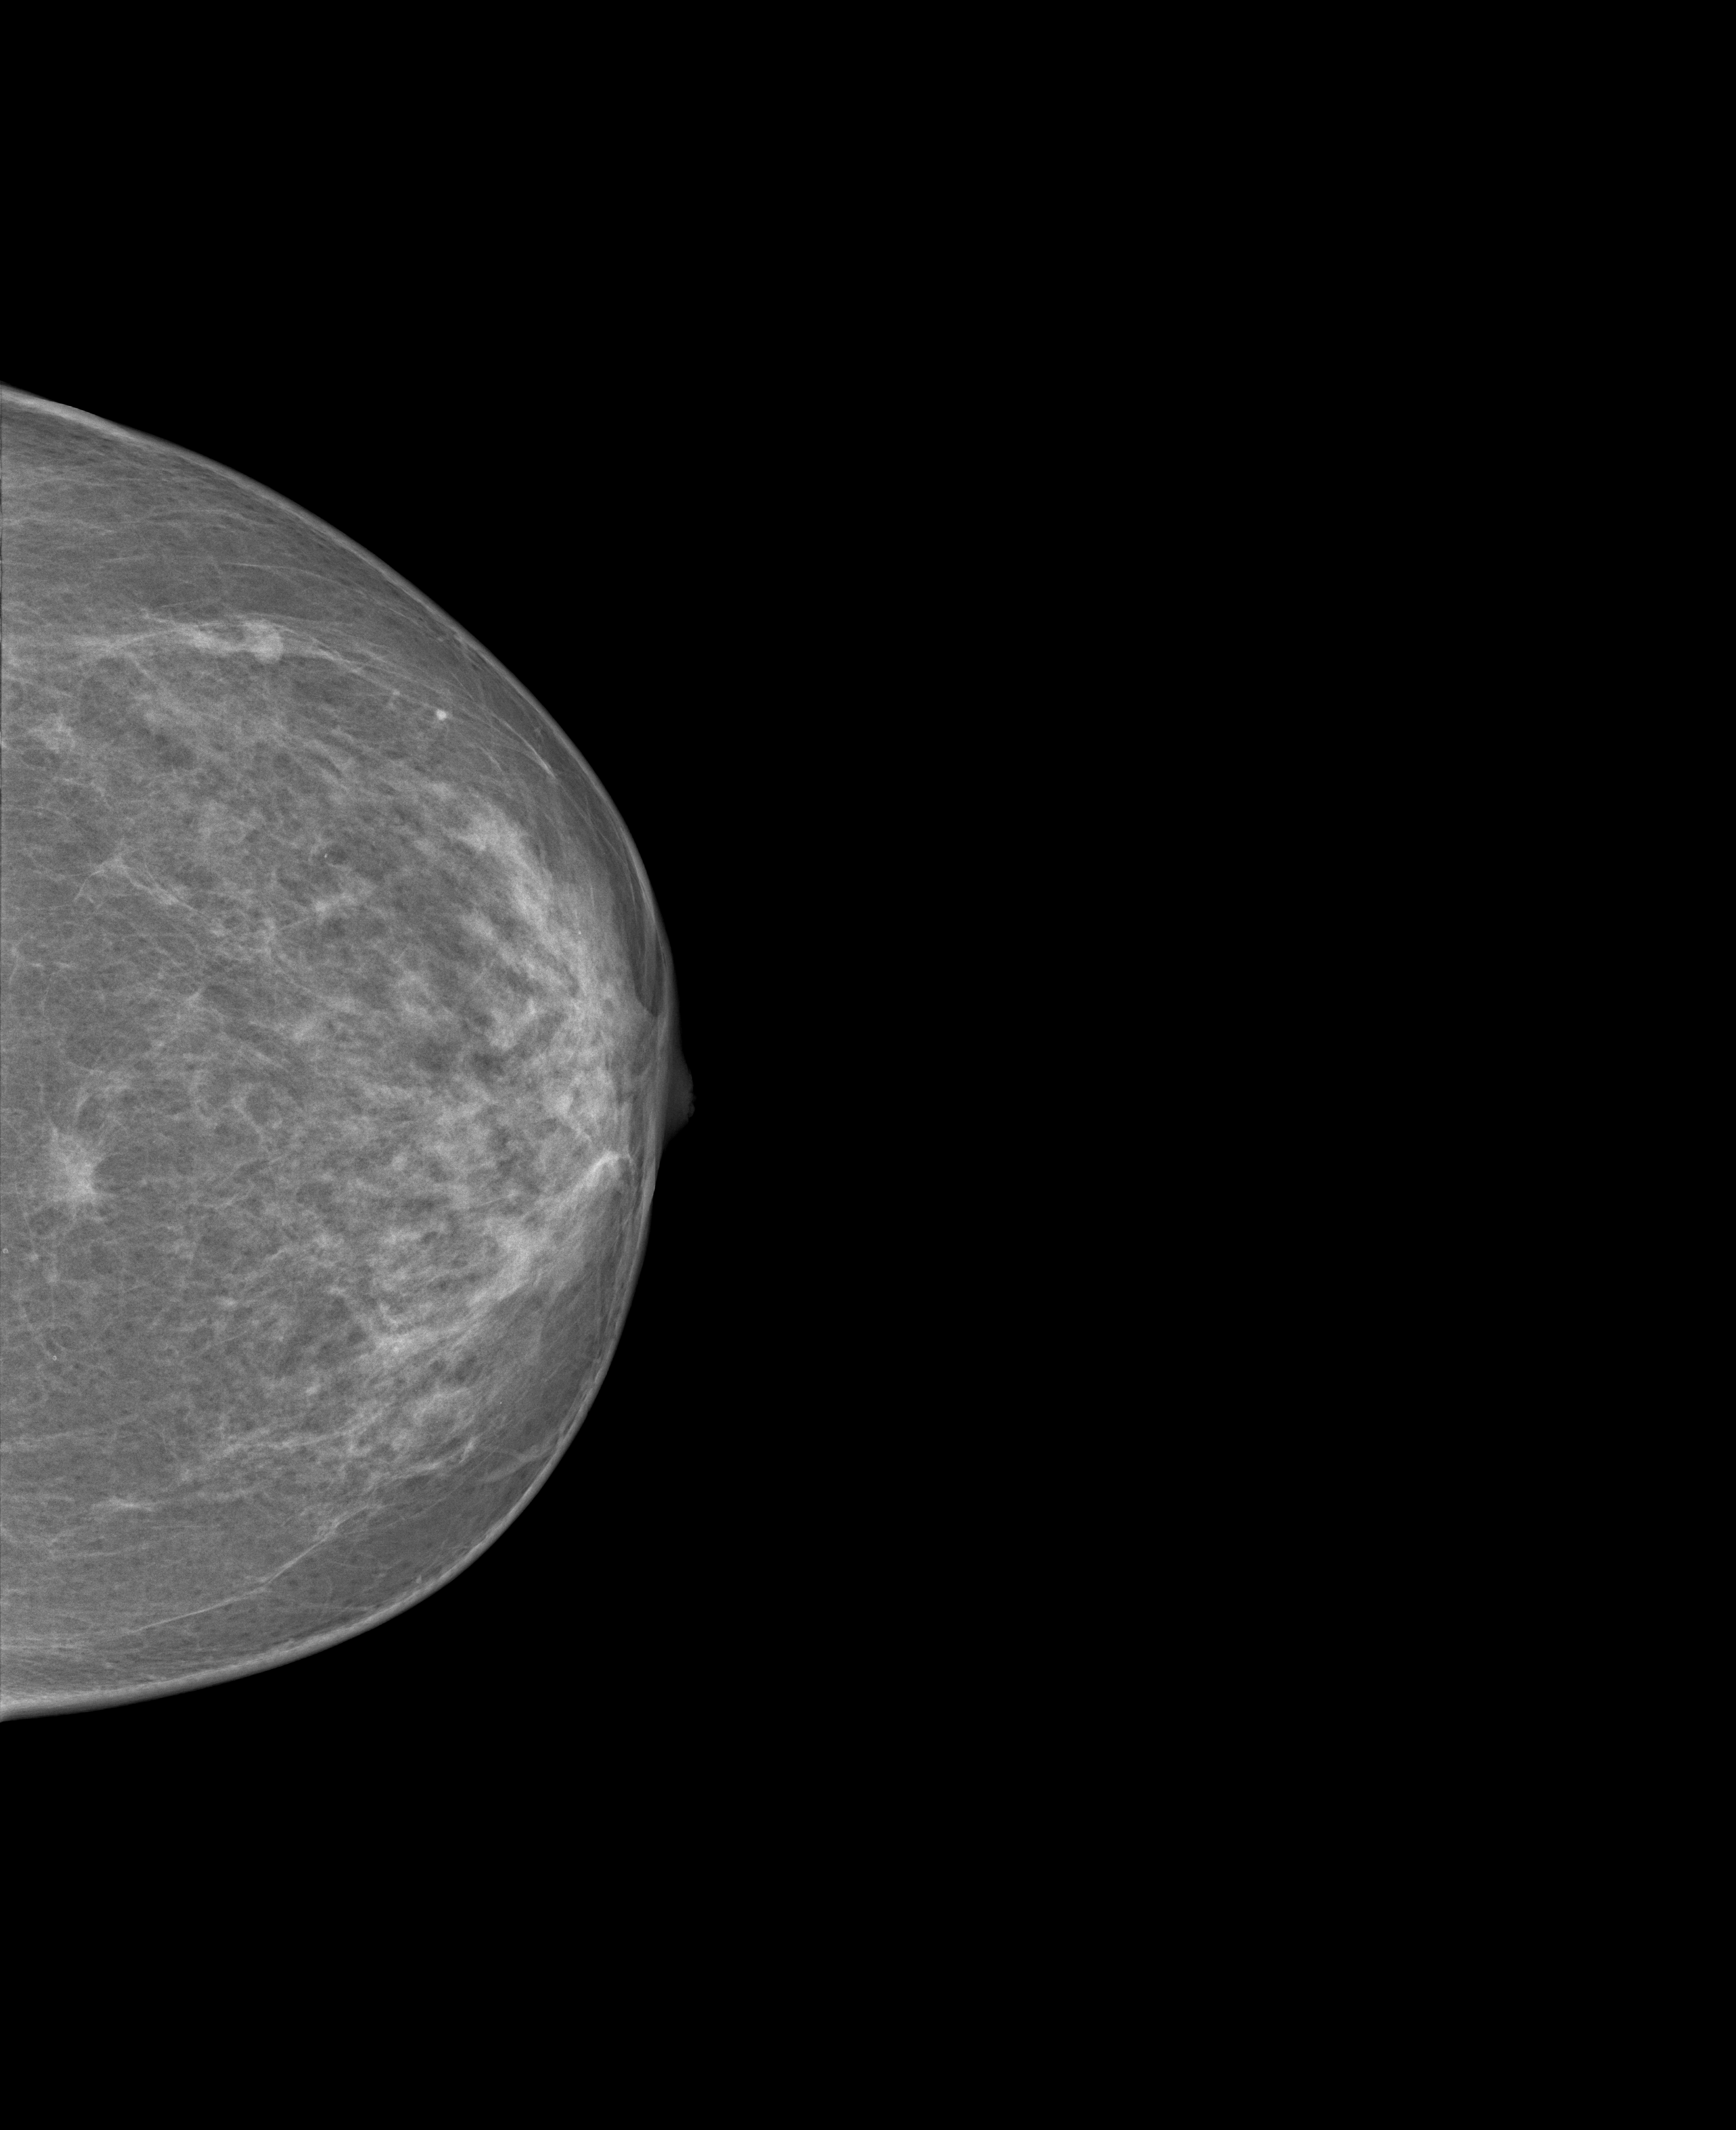
\includegraphics[height=3.5cm]{plots/mammogram_ex1.png}
			\end{subfigure}
			\begin{subfigure}{0.16\textwidth}
				\centering
					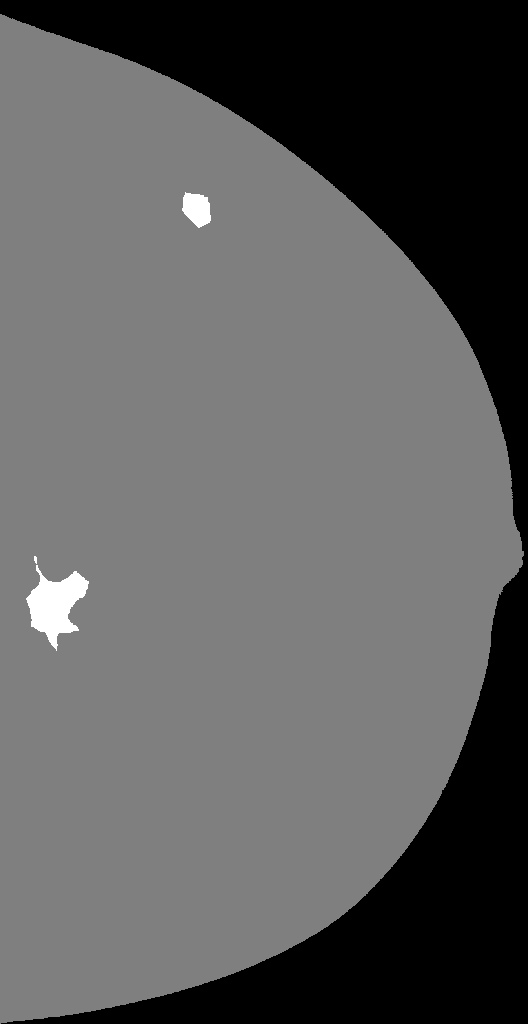
\includegraphics[height=3.5cm]{plots/label_ex1.png}
			\end{subfigure}
			\begin{subfigure}{0.17\textwidth}
				\centering
					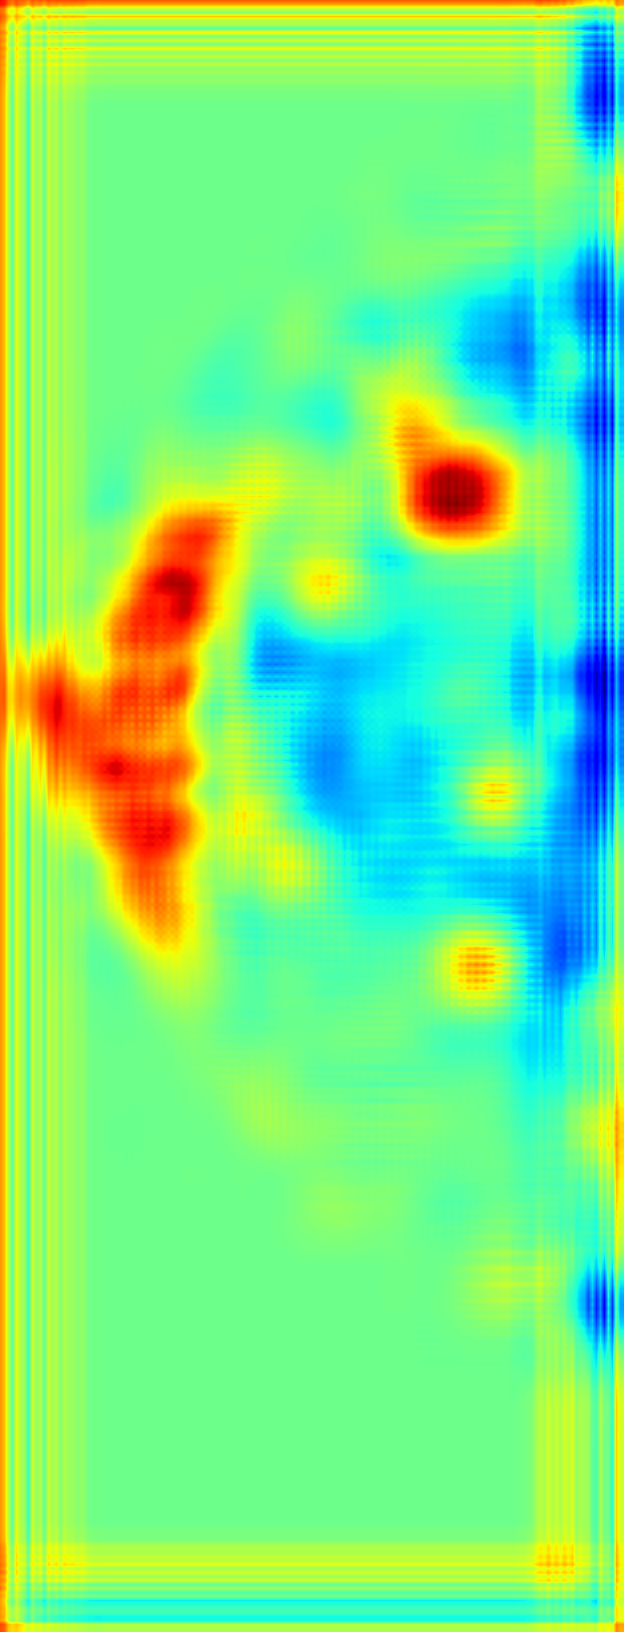
\includegraphics[height=3.5cm]{plots/logits_ex1_v3.png}
			\end{subfigure}
			\begin{subfigure}{0.22\textwidth}
				\centering
					
\includegraphics[height=3.5cm]{plots/segmentation_ex1_v3.png}
			\end{subfigure}% img_108_146_1_RCC.png
			\\
			\begin{subfigure}{0.25\textwidth}
				\centering
					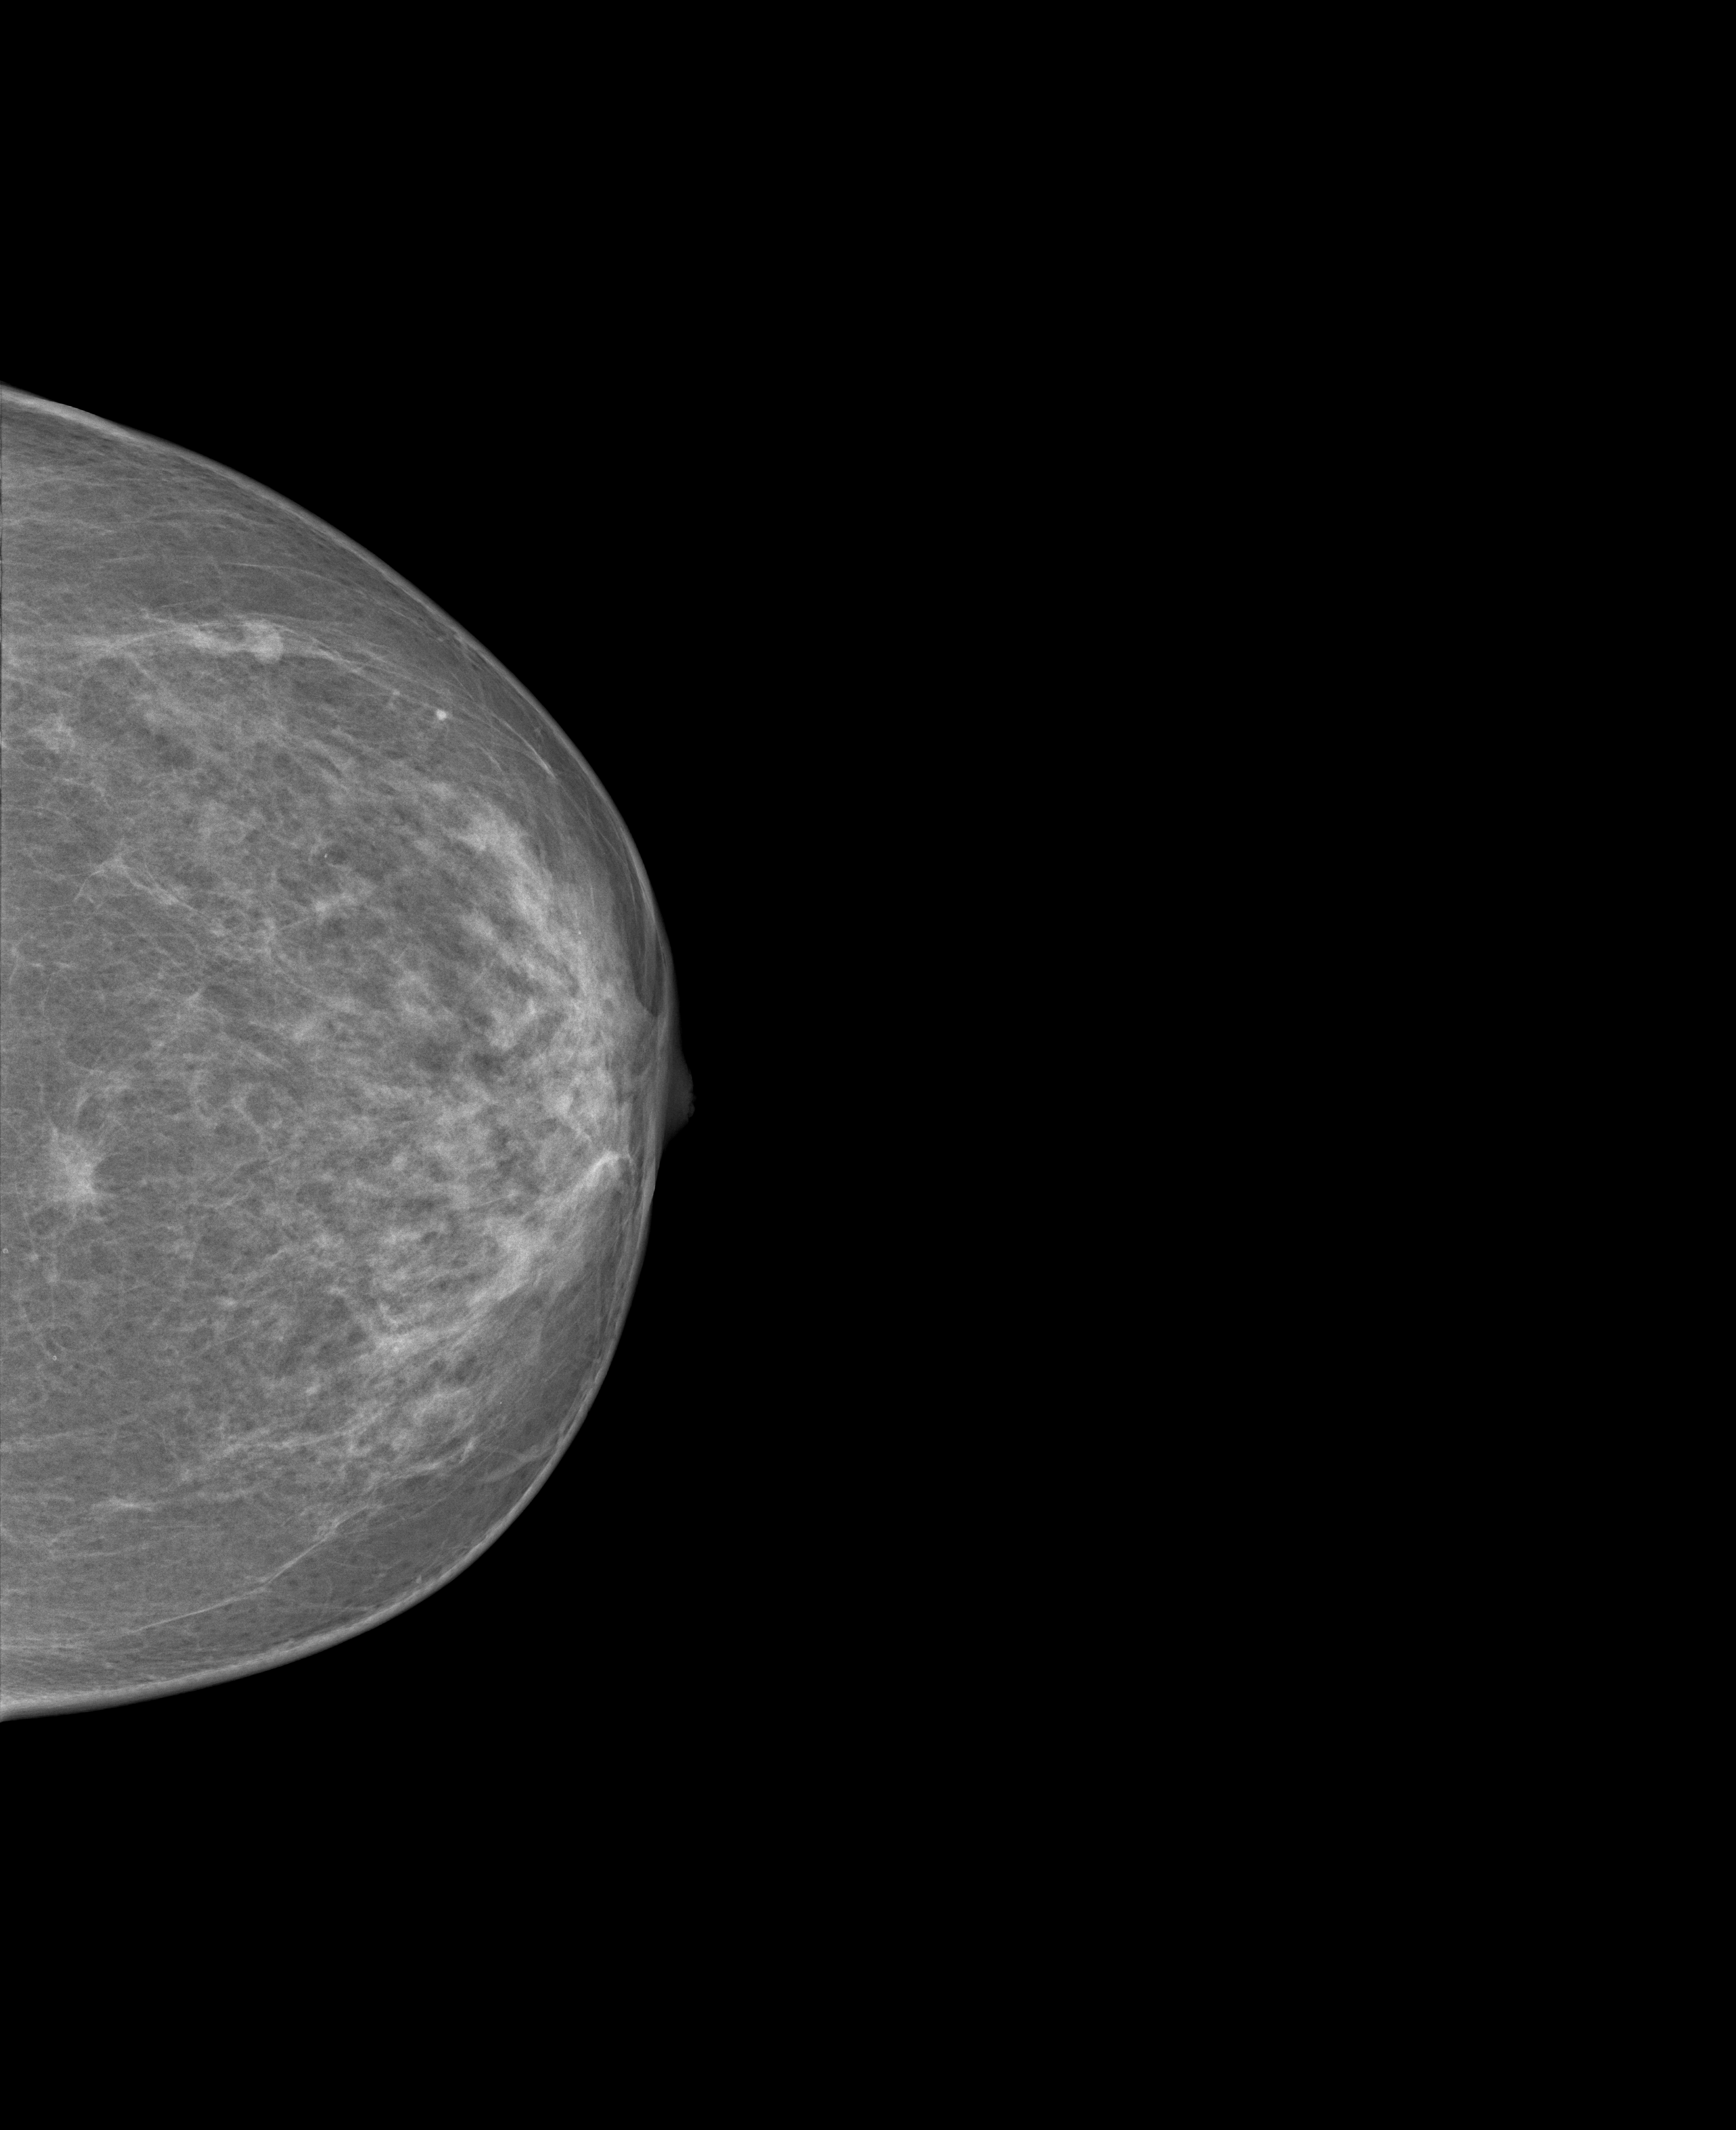
\includegraphics[height = 3.5cm]{plots/mammogram_ex2.png}
				\caption{Original}
			\end{subfigure}
			\begin{subfigure}{0.16\textwidth}
				\centering
					\includegraphics[height = 3.5cm]{plots/label_ex2.png}
				\caption{Label}
			\end{subfigure}
			\begin{subfigure}{0.17\textwidth}
				\centering
					\includegraphics[height = 3.5cm]{plots/logits_ex2_v3.png}
				\caption{Prediction}
			\end{subfigure}
			\begin{subfigure}{0.22\textwidth}
				\centering
					\includegraphics[height = 3.5cm]{plots/segmentation_ex2_v3.png}
				\caption{Segmentation}
			\end{subfigure}%img_251_334_1_LCC.png
		\end{figure}		
	\end{frame}
	
	\begin{frame}
		\frametitle{Writing the thesis}
		65 pages...
	\end{frame}
	
	
	\section[Future work]{Future work}
	\begin{frame}
		\frametitle{Future work}
		\begin{itemize}
			\item Write the thesis
			\item ?
		\end{itemize}
	\end{frame}

	\begin{frame}[c]
		\begin{center}
		\Huge Questions
		\end{center}
	\end{frame}

\end{document}
